%%%%%%%%%%%%%%%%%%%%%%%%%%%%%%%%%%%%%%%%%
% Beamer Presentation
% LaTeX Template
% Version 2.0 (March 8, 2022)
%
% This template originates from:
% https://www.LaTeXTemplates.com
%
% Author:
% Vel (vel@latextemplates.com)
%
% License:
% CC BY-NC-SA 4.0 (https://creativecommons.org/licenses/by-nc-sa/4.0/)
%
%%%%%%%%%%%%%%%%%%%%%%%%%%%%%%%%%%%%%%%%%

%----------------------------------------------------------------------------------------
%	PACKAGES AND OTHER DOCUMENT CONFIGURATIONS
%----------------------------------------------------------------------------------------

\documentclass[
	11pt, % Set the default font size, options include: 8pt, 9pt, 10pt, 11pt, 12pt, 14pt, 17pt, 20pt
	%t, % Uncomment to vertically align all slide content to the top of the slide, rather than the default centered
	%aspectratio=169, % Uncomment to set the aspect ratio to a 16:9 ratio which matches the aspect ratio of 1080p and 4K screens and projectors
]{beamer}

\graphicspath{{../figures/}{../}{./Images/}{./}} % Look for images in the paper's directories

\usepackage{booktabs} % Allows the use of \toprule, \midrule and \bottomrule for better rules in tables

%----------------------------------------------------------------------------------------
%	SELECT LAYOUT THEME
%----------------------------------------------------------------------------------------

\usetheme{CambridgeUS}

%----------------------------------------------------------------------------------------
%	SELECT COLOR THEME
%----------------------------------------------------------------------------------------

\usecolortheme{dolphin}

% set colors
\definecolor{myNewColorA}{RGB}{0, 0, 102}
\definecolor{myNewColorB}{RGB}{0, 75, 153}
\definecolor{myNewColorC}{RGB}{0, 153, 204} % {130,138,143}
\setbeamercolor*{palette primary}{bg=myNewColorC}
\setbeamercolor*{palette secondary}{bg=myNewColorB, fg = white}
\setbeamercolor*{palette tertiary}{bg=myNewColorA, fg = white}
\setbeamercolor*{titlelike}{fg=myNewColorA}
\setbeamercolor*{title}{bg=myNewColorA, fg = white}
\setbeamercolor*{item}{fg=myNewColorA}
\setbeamercolor*{caption name}{fg=myNewColorA}
\setbeamercolor{block title}{bg=blue!30,fg=black}
\usefonttheme{professionalfonts}
\usepackage{hyperref}
\usepackage{amsmath}
\usepackage{amssymb}

\definecolor{bluish}{RGB}{20, 22, 128}
\definecolor{prussian}{RGB}{0, 49, 83}
\definecolor{darkgreen}{RGB}{0,100,0}

%----------------------------------------------------------------------------------------
%	SELECT FONT THEME & FONTS
%----------------------------------------------------------------------------------------

\usefonttheme{default} % Typeset using the default sans serif font

%------------------------------------------------

\usepackage{palatino} % Use the Palatino font for serif text
\usepackage[default]{FiraSans} % Use the Fira Sans font for sans serif text

%----------------------------------------------------------------------------------------
%	SELECT INNER THEME
%----------------------------------------------------------------------------------------

\useinnertheme{circles}

%----------------------------------------------------------------------------------------
%	PRESENTATION INFORMATION
%----------------------------------------------------------------------------------------
\usepackage[
backend=biber,
style=alphabetic,
sorting=ynt
]{biblatex}
\addbibresource{references.bib}

\newcommand{\M}{\mathcal{M}}

\title[Bouquet2D]{Bouquet: A Visualization Tool for Symmetry Sets and Vineyards}

\author[Rohit Roy]{Erin Chambers, Christopher Fillmore, Shankha Shubhra Mukherjee, \textcolor{myNewColorC}{\textbf{Rohit Roy}}, Elizabeth Stephenson, Mathijs Wintraecken}

\date[EuroCG 2026]{EuroCG 2026}

%----------------------------------------------------------------------------------------

\begin{document}

%----------------------------------------------------------------------------------------
%	TITLE SLIDE
%----------------------------------------------------------------------------------------

\begin{frame}
	\titlepage
\end{frame}

%----------------------------------------------------------------------------------------
%	OUTLINE
%----------------------------------------------------------------------------------------

\begin{frame}{Outline}
	\tableofcontents
\end{frame}

%----------------------------------------------------------------------------------------
%	PRESENTATION BODY SLIDES
%----------------------------------------------------------------------------------------

\section{Motivation}

\begin{frame}{Motivation}
    \begin{itemize}
        \item The \textbf{Persistent Homology Transform (PHT)} is a powerful topological summary for shape analysis.
        \pause
        \item We study a variant: the \textbf{Radial Persistence Transform (RPT)}.
        \begin{itemize}
            \item Given a manifold $\M \subset \mathbb{R}^d$ and a point $x$, consider the squared distance function restricted to $\M$:
            \[
            f_x = d_{\mathbb{E}}^2(\cdot, x)\big|_{\M}
            \]
            \item The RPT maps $x \mapsto \mathrm{Dgm}(f_x)$ (persistence diagram).
        \end{itemize}
        \pause
        \item \textbf{Key fact} (Bruce--Giblin--Gibson, Porteous): The topology of $f_x$ changes precisely when $x$ crosses the \textbf{symmetry set} or \textbf{focal set}.
        \pause
        \item \textbf{Central question:} How is the topology of the symmetry/focal sets related to the topology of the vineyard?
    \end{itemize}
\end{frame}

\begin{frame}{Our Contribution}
    We present \textbf{Bouquet2D}, an interactive web-based 2D visualization tool to study this relationship.

    \bigskip

    \begin{itemize}
        \item Computes and visualizes \textbf{focal sets} (evolutes) and \textbf{symmetry sets} of user-defined curves.
        \pause
        \item Tracks the evolution of persistence diagrams along a loop $\gamma$, forming a \textbf{vineyard}.
        \pause
        \item Reveals \textbf{braiding patterns} and \textbf{monodromy} recently characterized in Chambers et al.\ [SODA 2026].
        \pause
        \item Real-time spline-based interface: deform $\M$ and observe geometric bifurcations as topological events.
    \end{itemize}

    \bigskip
    \centering
    \url{https://www.rohitroy.me/symmetry-set-visualizer/bouquet2d.html}
\end{frame}

%----------------------------------------------------------------------------------------

\section{Preliminaries}

\begin{frame}{Focal Set (Evolute)}
    Let $\M$ be a smooth plane curve parameterized by arc length $s$, with unit tangent $\mathbf{t}(s)$ and unit normal $\mathbf{n}(s)$.

    \begin{itemize}
        \item \textbf{Curvature:} $\mathbf{t}'(s) = \kappa(s)\,\mathbf{n}(s)$
        \item \textbf{Radius of curvature:} $\rho(s) = 1/\kappa(s)$
    \end{itemize}

    \begin{definition}[Evolute]
    The \textbf{evolute} (focal set) of $\M$ is the locus of centers of osculating circles:
    \[
    E(s) = \gamma(s) + \rho(s)\,\mathbf{n}(s)
    \]
    \end{definition}

    \pause
    \begin{definition}[Symmetry Set]
    The \textbf{symmetry set} $\mathrm{sym}(\M)$ is the closure of the set of centers $p$ such that a ball $B(p,r)$ is tangent to $\M$ in at least two places.
    \end{definition}
\end{frame}

\begin{frame}{Focal and Symmetry Set: Example}
    \begin{figure}
        \centering
        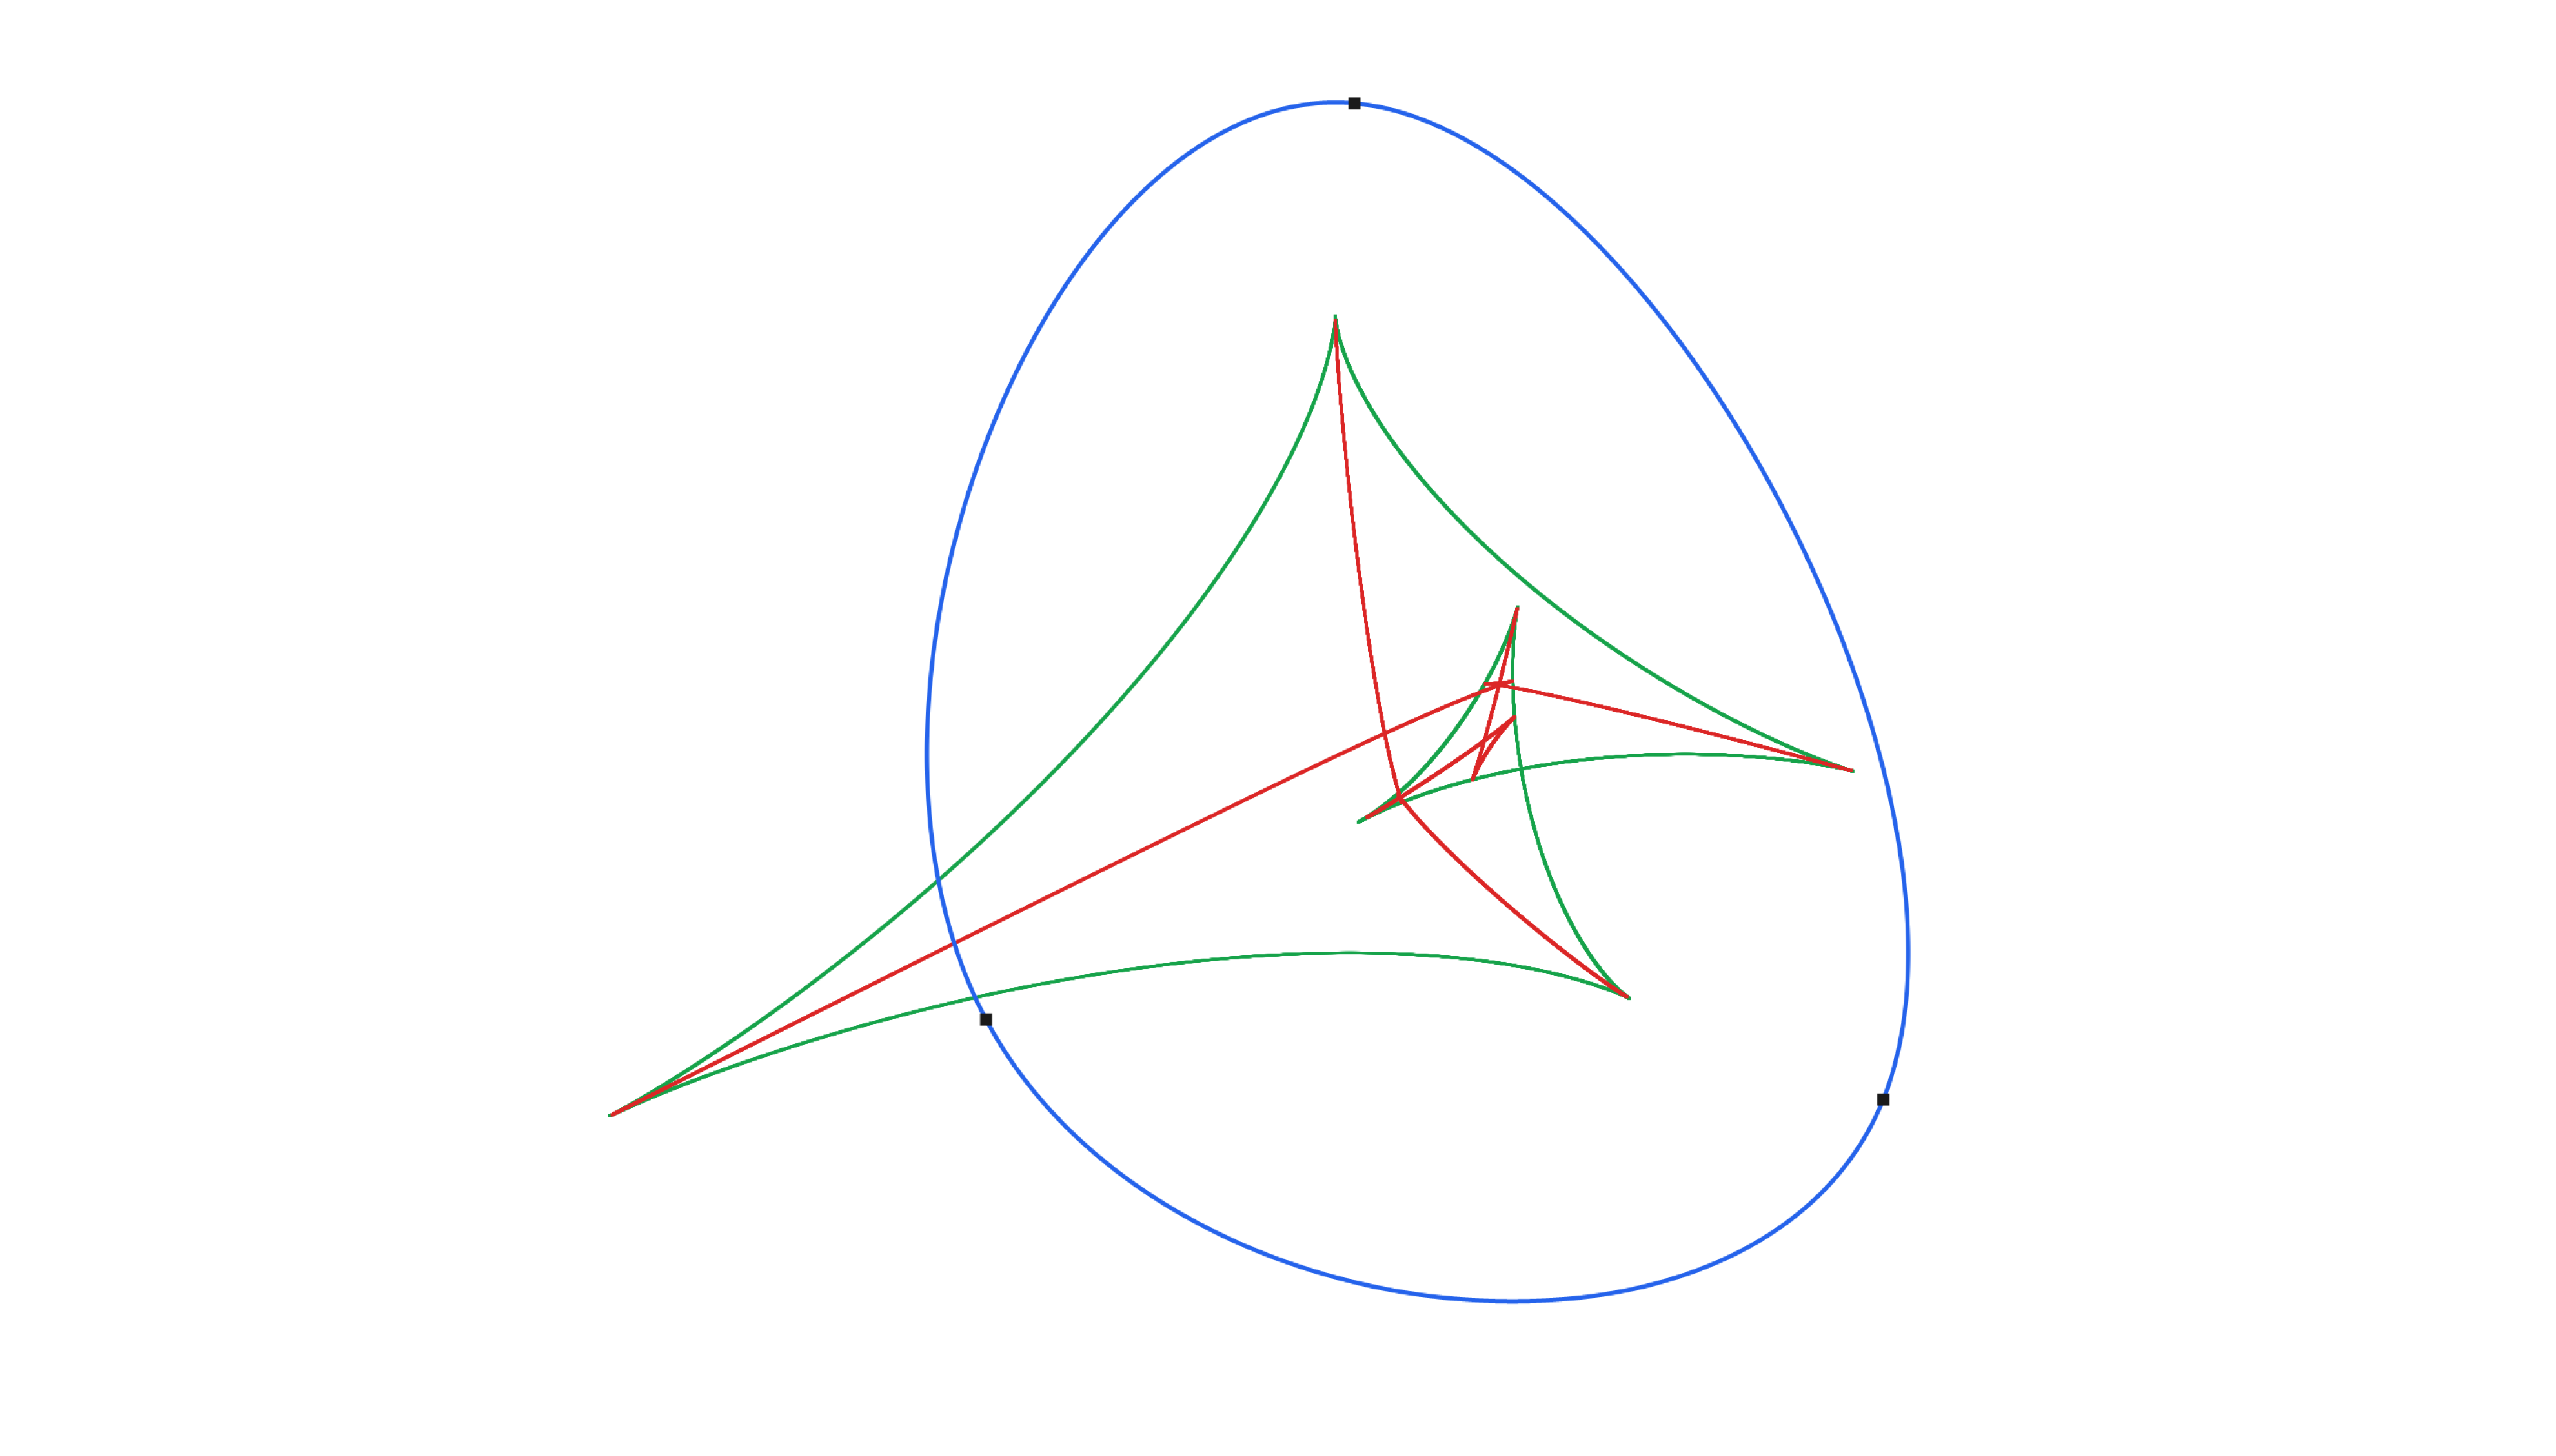
\includegraphics[width=0.75\textwidth]{focal_symmetry1.pdf}
        \caption{Focal set (green) and symmetry set (red) of a spline-defined curve $\M$.}
    \end{figure}
\end{frame}

\begin{frame}{Vineyards}
    Let $\gamma: S^1 \to \mathbb{R}^2$ be a closed curve. For each $t \in S^1$, define:
    \[
    f_t(x) = d_{\mathbb{E}}^2(x, \gamma(t))\big|_{\M}
    \]

    \begin{definition}[Vineyard]
    The \textbf{vineyard} $\mathcal{V}(\M, \gamma)$ is the union:
    \[
    \mathcal{V}(\M, \gamma) = \bigcup_{t \in S^1} \{t\} \times \mathrm{Dgm}(f_t)
    \]
    It decomposes into continuous curves called \textbf{vines}.
    \end{definition}

    \pause
    \begin{definition}[Monodromy]
    Following a vine for one full period of $S^1$ may not return to the same persistence point. If the smallest $k > 1$ periods are needed to return, the monodromy has \textbf{order $k$}.
    \end{definition}
\end{frame}

%----------------------------------------------------------------------------------------

\section{Algorithm}

\begin{frame}{Symmetry Set Computation}
    Given sampled points $\mathcal{P} = \{p_1, \dots, p_k\}$ from $\M$ with tangents $\{t_i\}$ and normals $\{n_i\}$:

    \begin{enumerate}
        \item \textbf{Bitangency detection:} For each pair $(i,j)$, check sign changes in
        \[
        f_{\pm}(i,j) = (p_i - p_j) \cdot (t_i \pm t_j)
        \]
        \pause
        \item \textbf{Normal intersection:} When a sign change is detected, find the center $C$ by intersecting normal lines:
        \[
        \lambda = \frac{-(p_i - p_j) \cdot (n_i \pm n_j)}{\|n_i \pm n_j\|^2}, \quad C = p_i + \lambda\, n_i
        \]
        \pause
        \item \textbf{Validation:} Keep $C$ only if $\big|\|C - p_i\| - \|C - p_j\|\big| < \epsilon_{\mathrm{rad}}$ (equidistance check).
    \end{enumerate}
\end{frame}

\begin{frame}{Vineyard Computation}
    \begin{itemize}
        \item Parameterize the source point $\gamma(t)$ along a \textbf{circular path} (user-defined radius/center) or an \textbf{arbitrary spline loop}.
        \pause
        \item For each fixed $t$:
        \begin{enumerate}
            \item Compute squared distances $f_t(p) = d_{\mathbb{E}}^2(p, \gamma(t))$ for all $p \in \mathcal{P}$.
            \item Sort points by distance and apply \textbf{Union-Find} on the lower-star filtration.
            \item Apply the \textbf{Elder Rule} to pair birth/death times.
        \end{enumerate}
        \pause
        \item Collect birth-death pairs across $m$ samples of $t \in S^1$ to form the vines.
        \item Visualize the resulting vineyard in 3D: $(t, \text{birth}, \text{death})$.
    \end{itemize}
\end{frame}

%----------------------------------------------------------------------------------------

\section{Examples and Demonstration}

\begin{frame}{Deforming Ellipses}
    Validation against known geometric behaviors:
    \begin{figure}
        \centering
        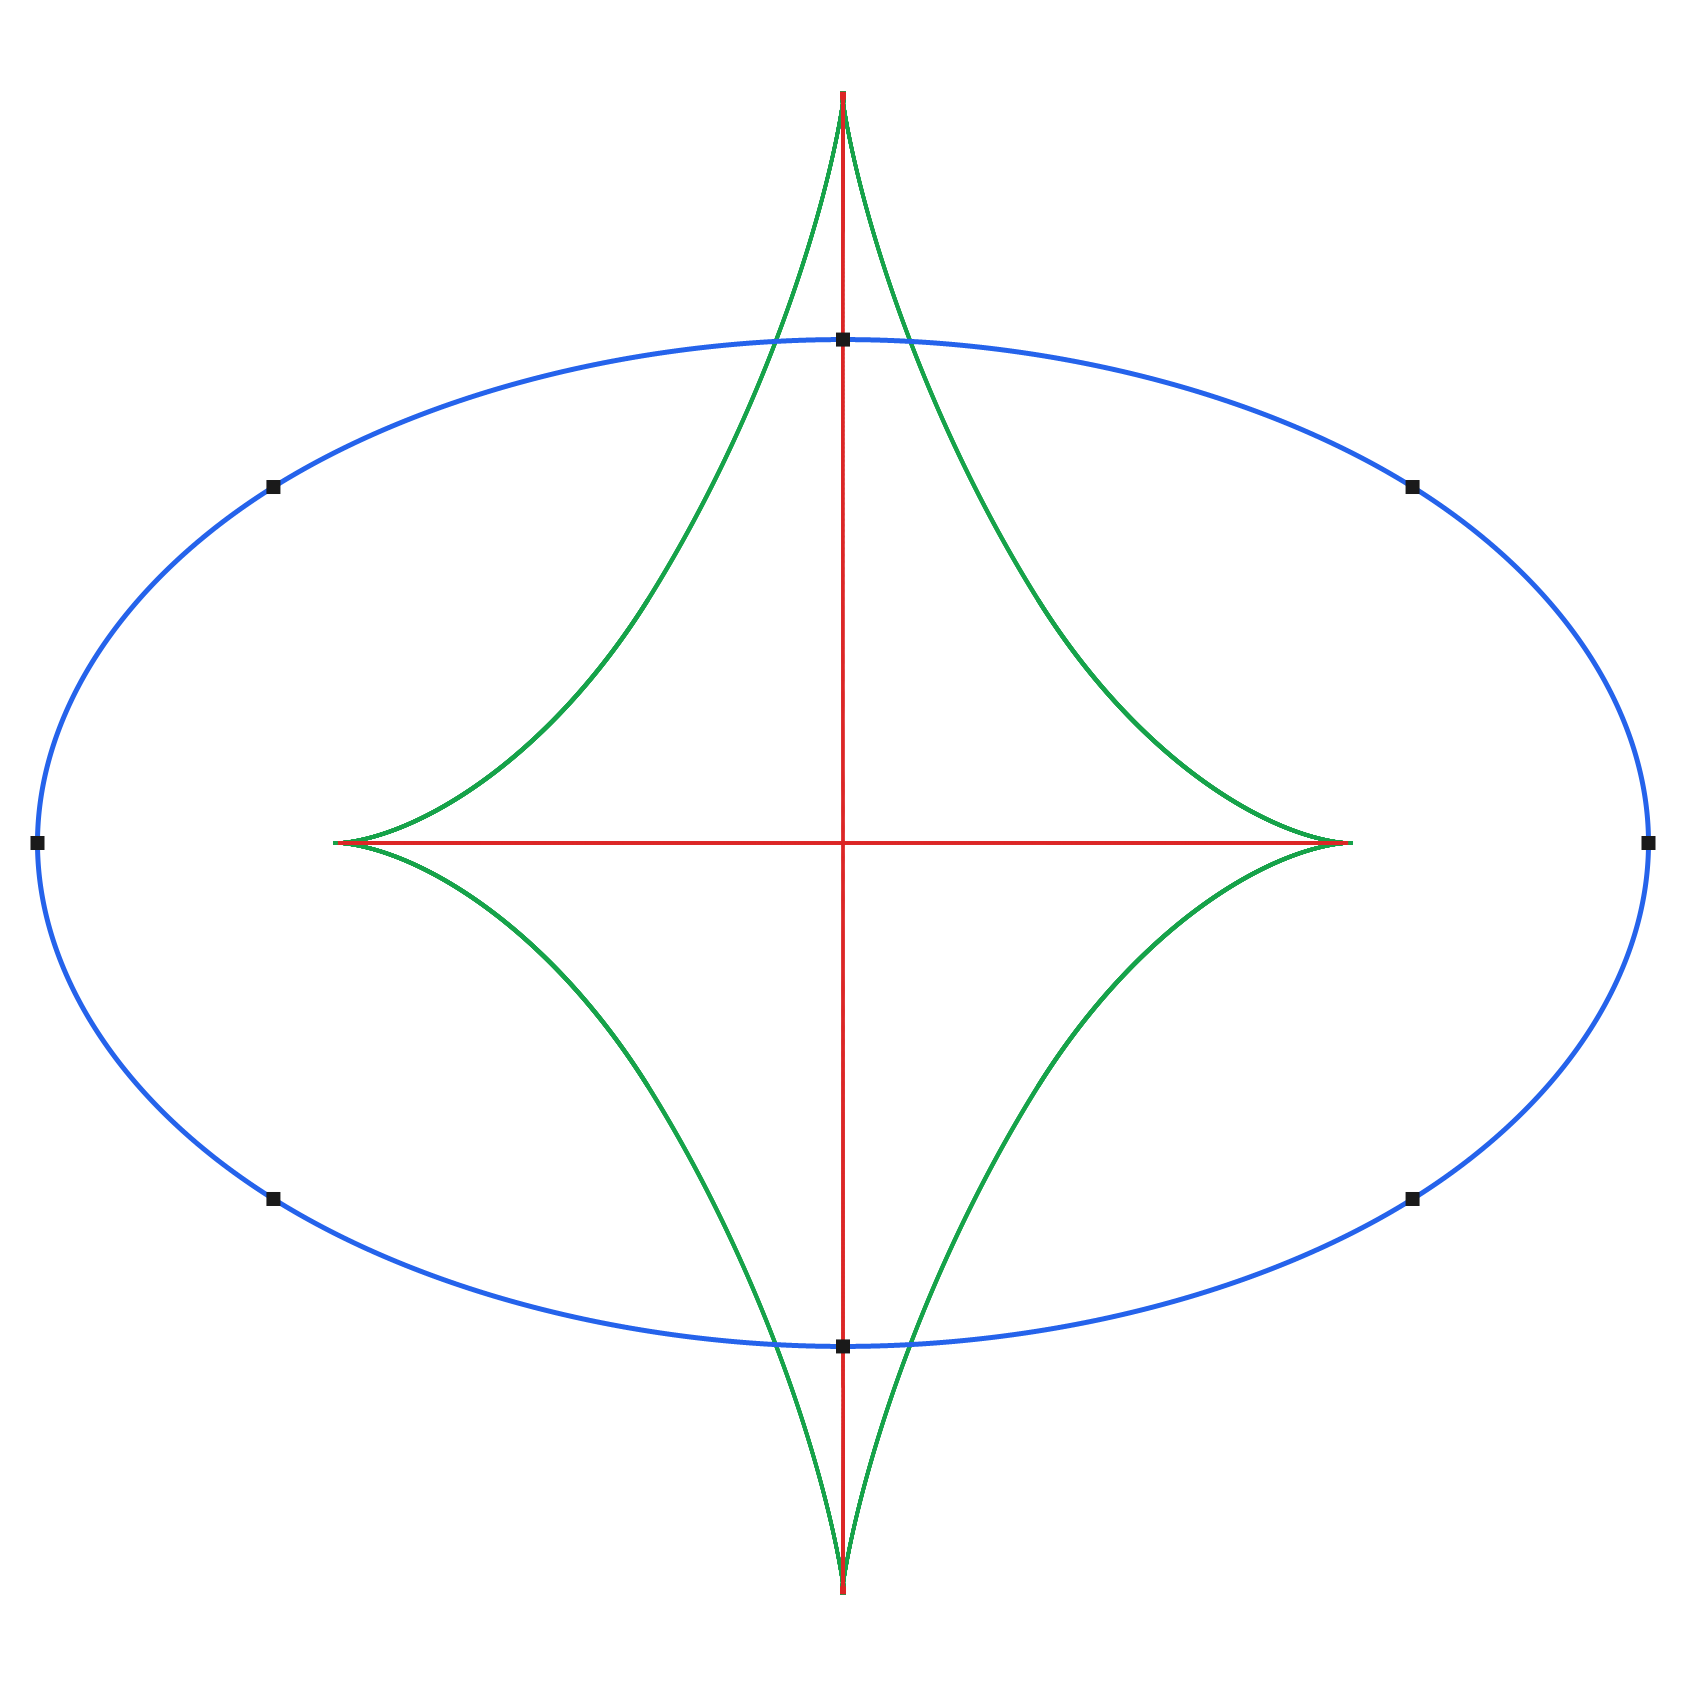
\includegraphics[width=0.42\linewidth]{ellipse_deform1.png}
        \hfill
        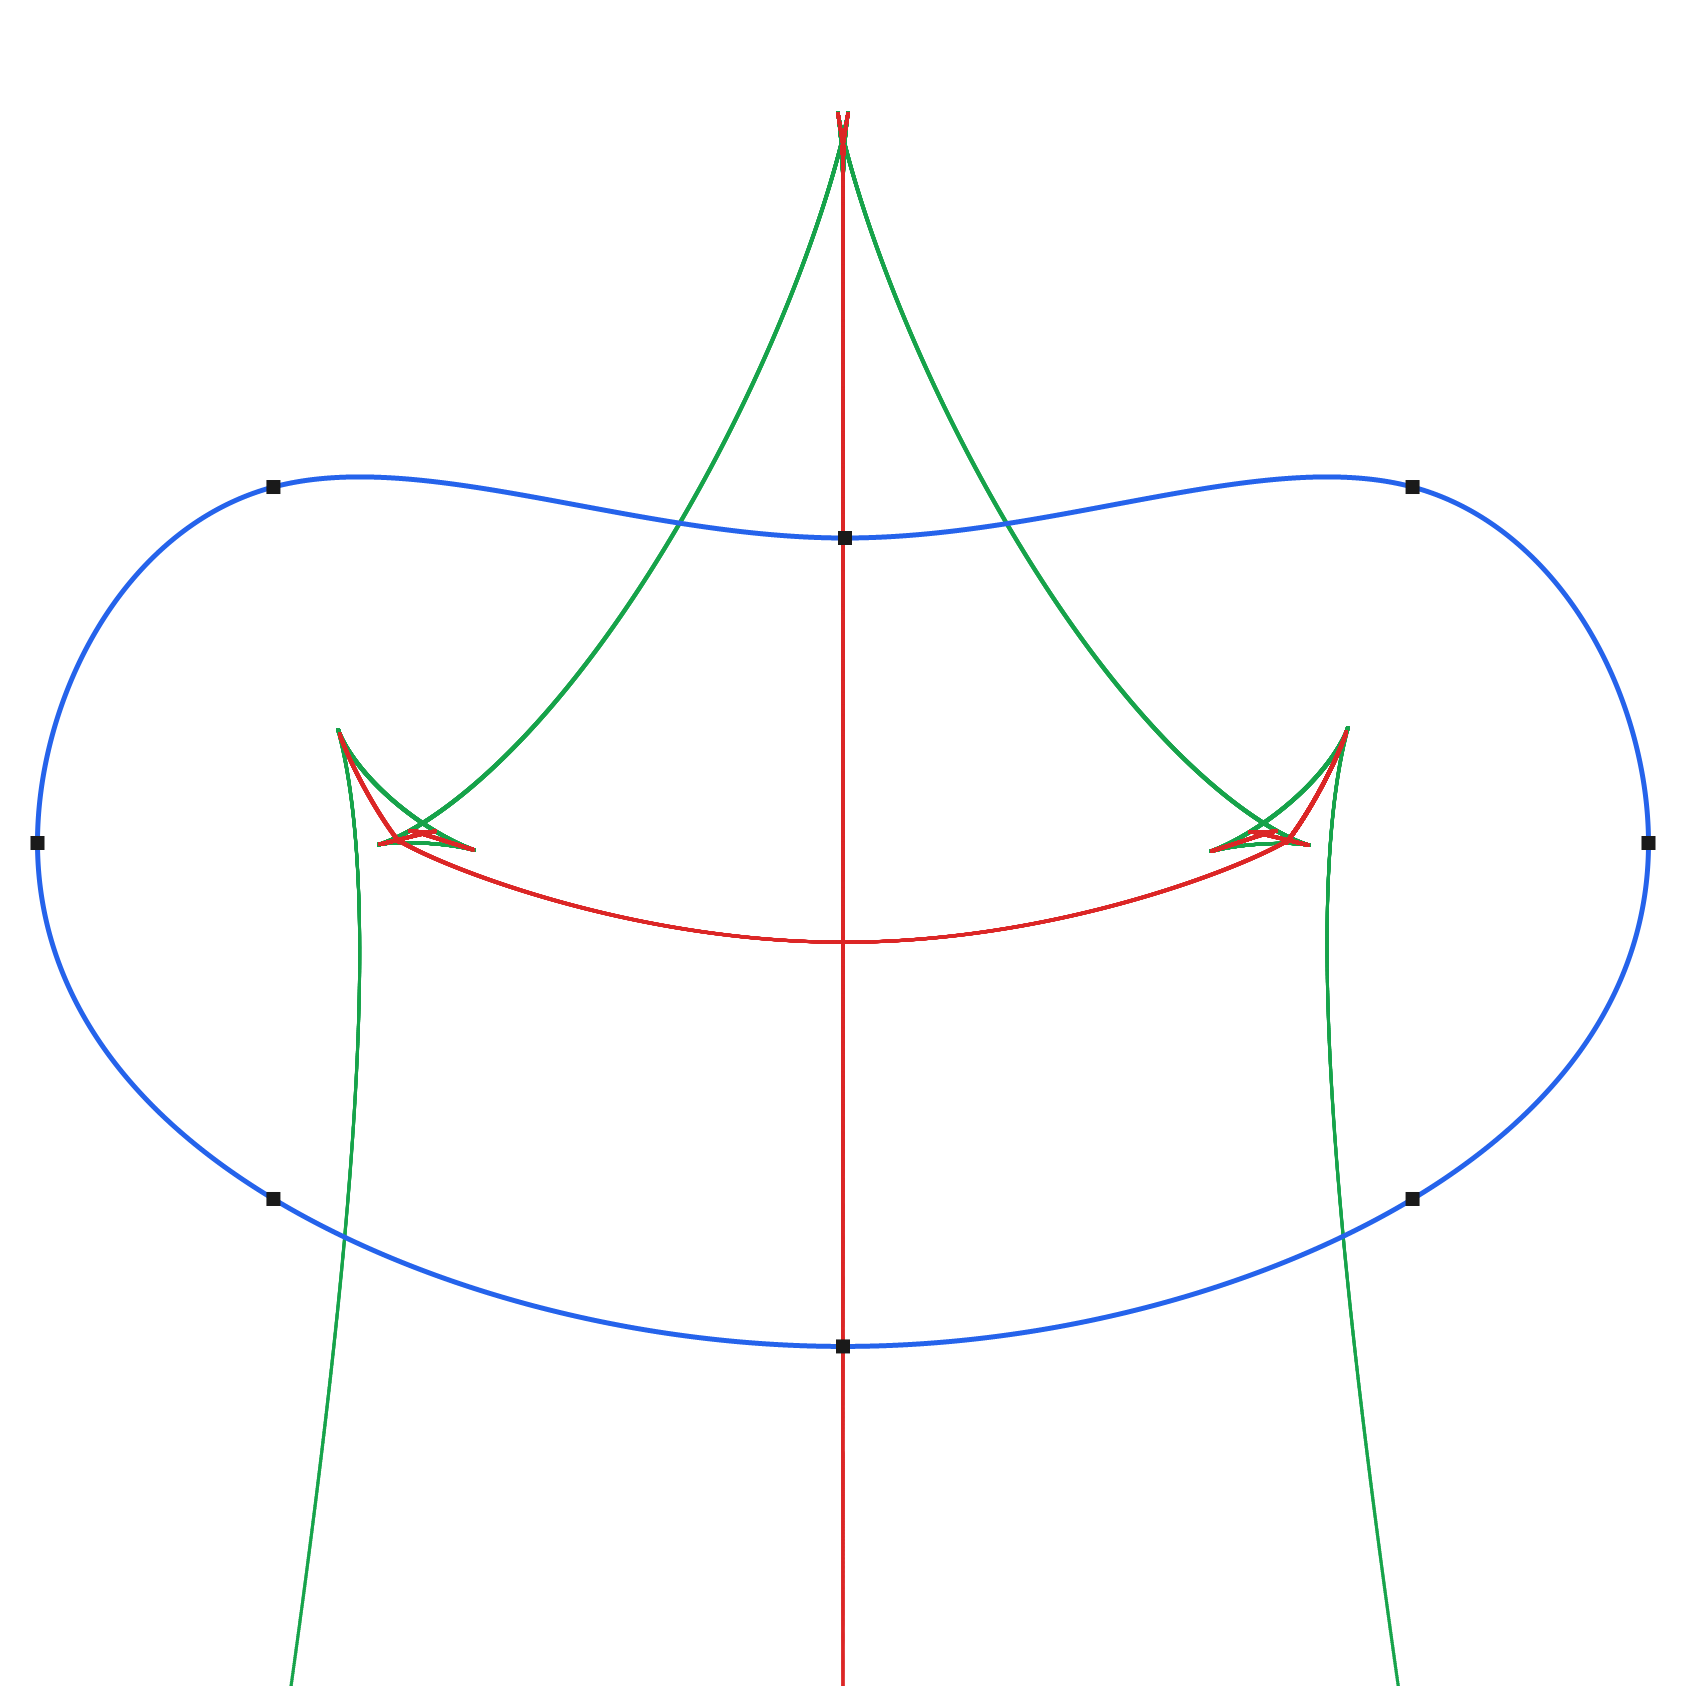
\includegraphics[width=0.42\linewidth]{ellipse_deform2.png}

        \vspace{0.3em}

        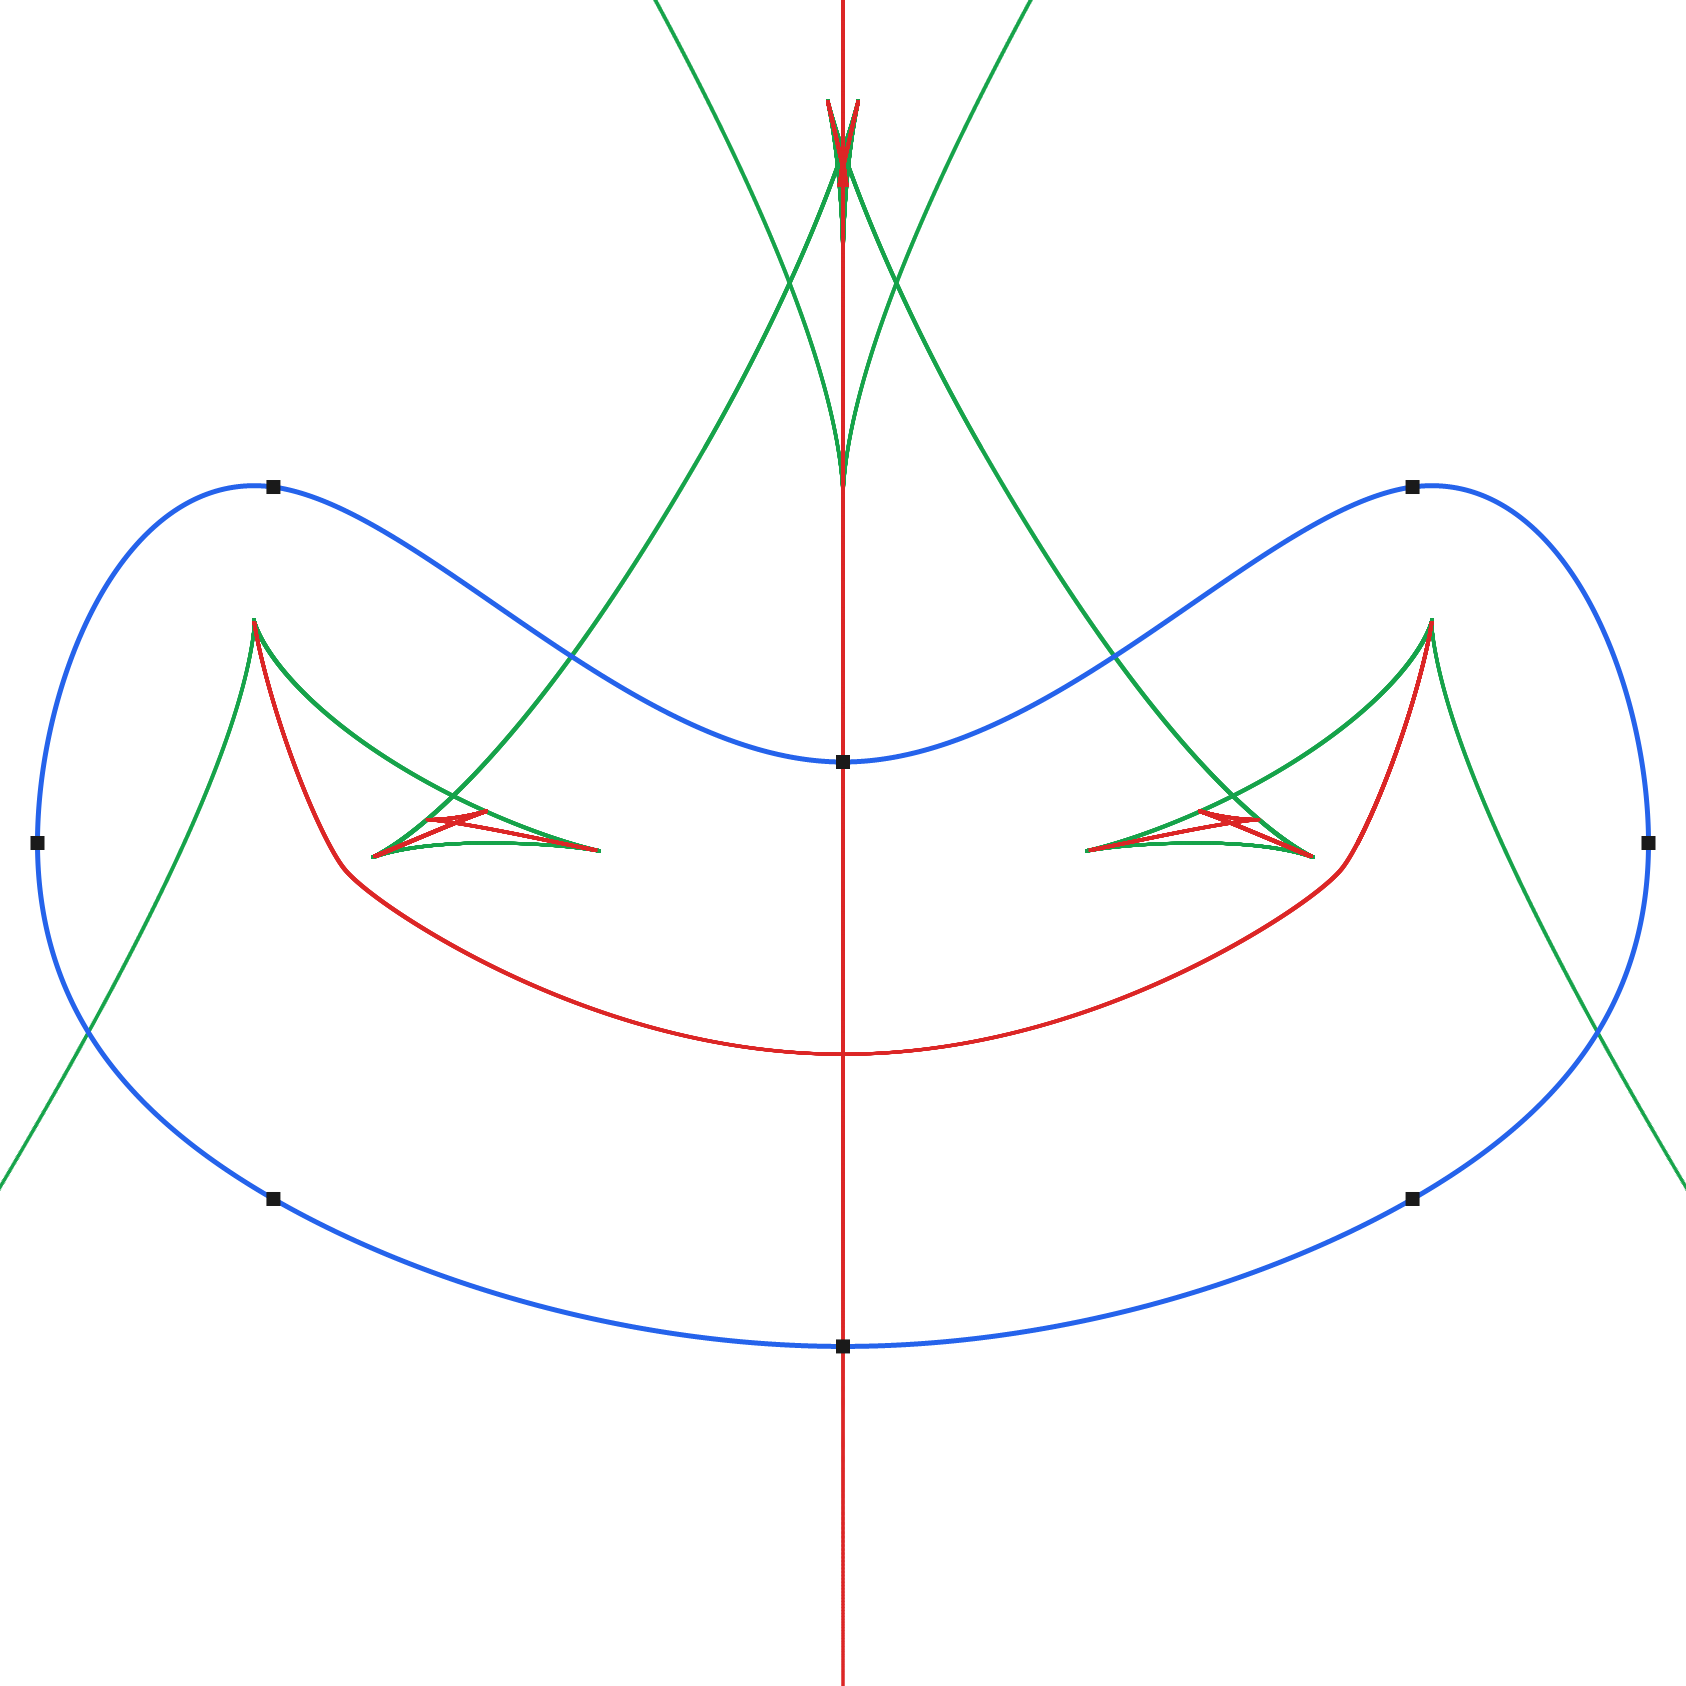
\includegraphics[width=0.42\linewidth]{ellipse_deform3.png}
        \hfill
        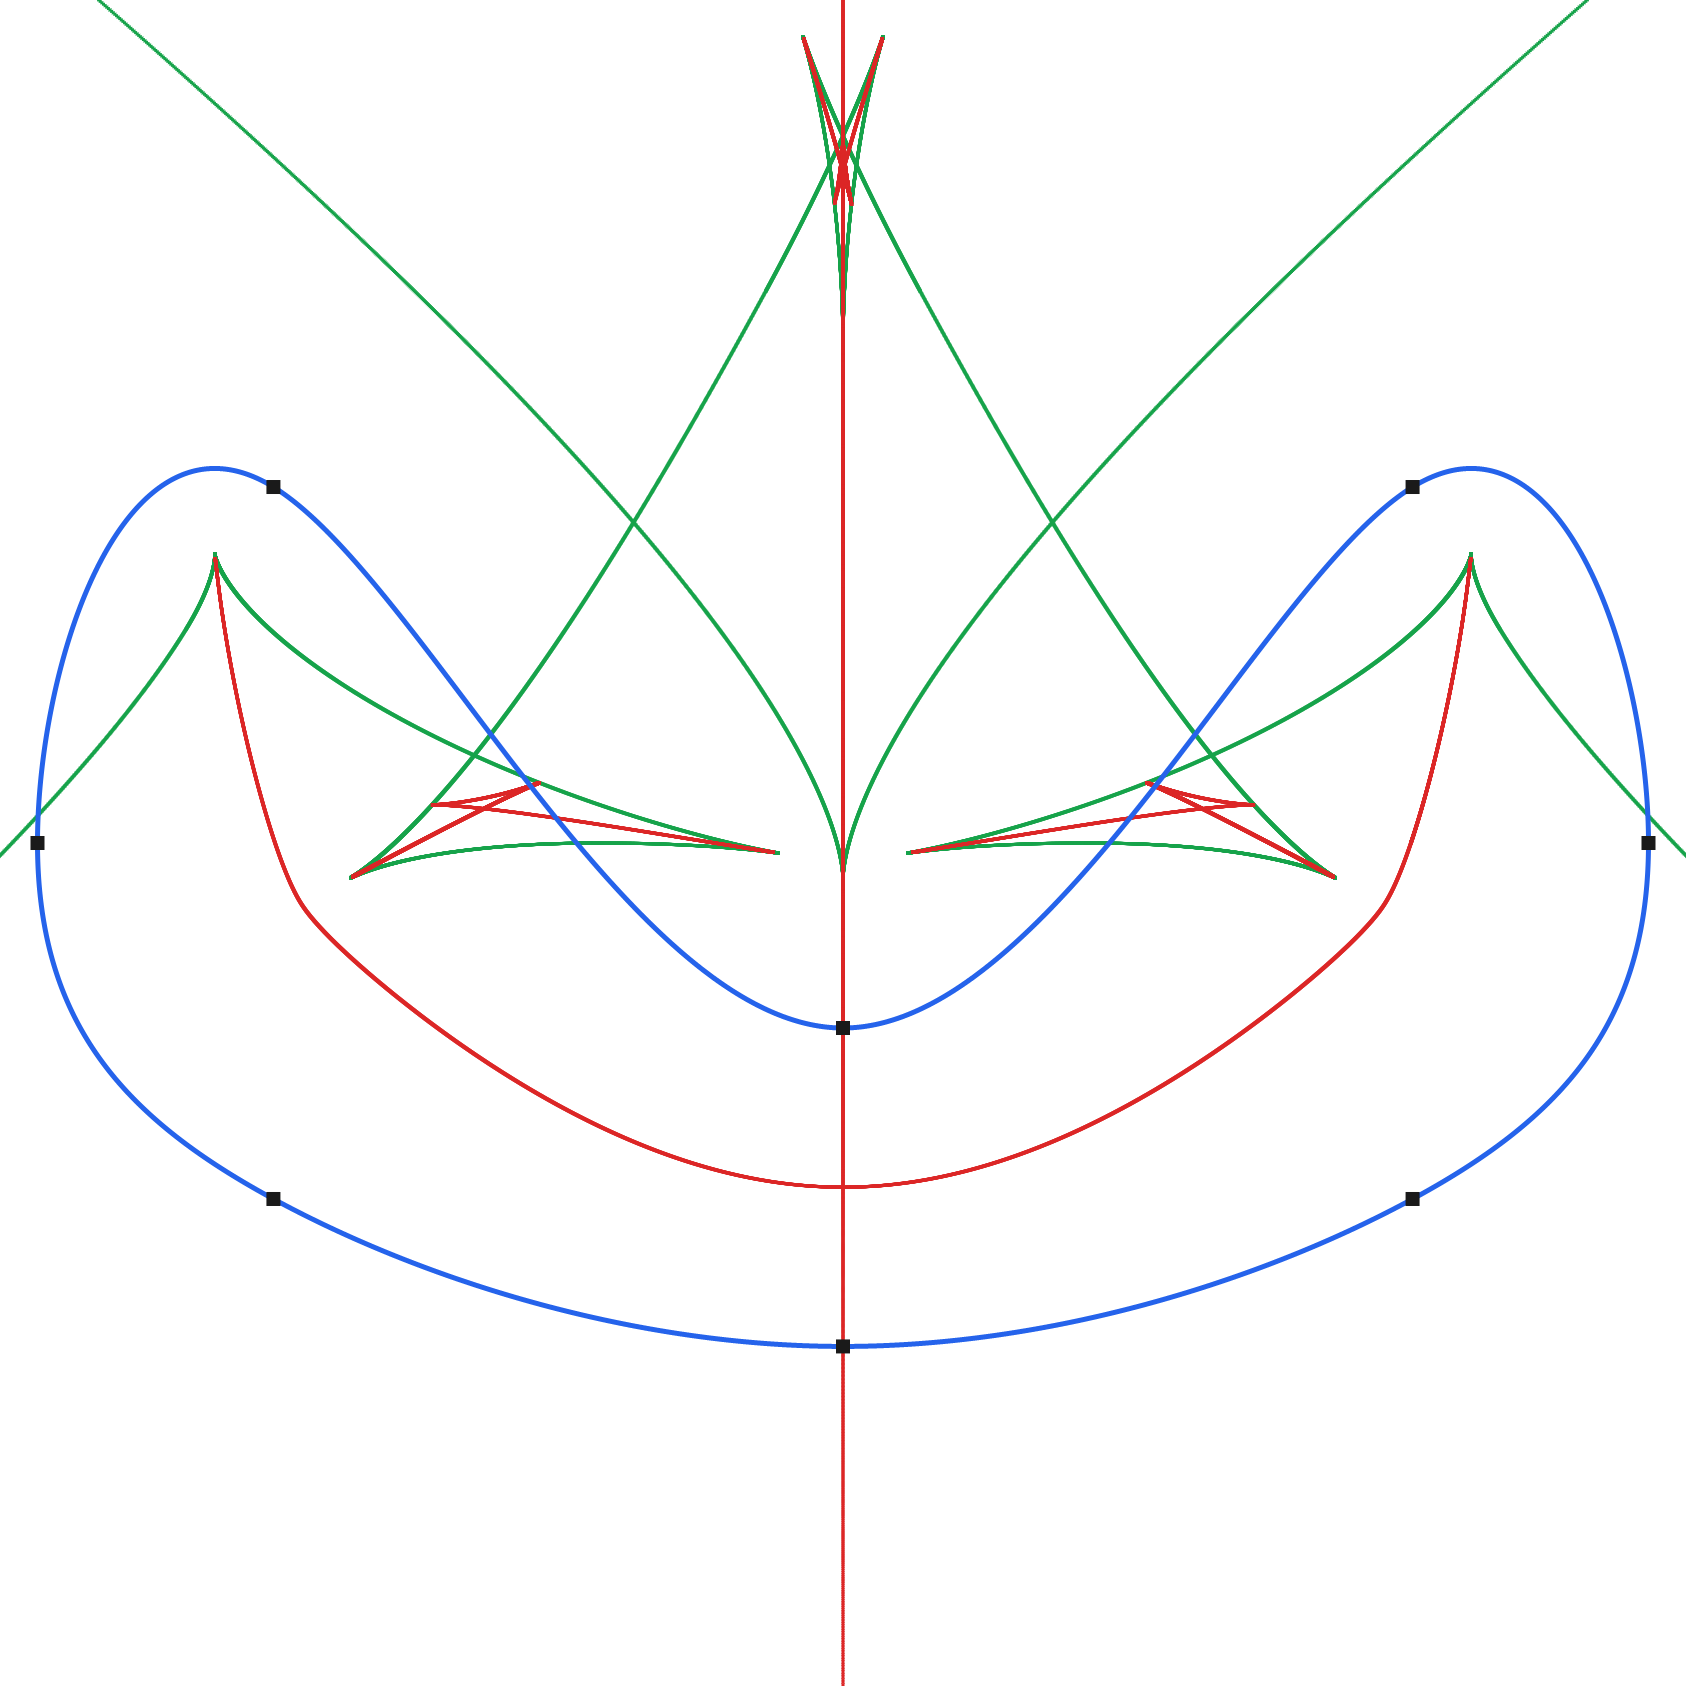
\includegraphics[width=0.42\linewidth]{ellipse_deform4.png}
        \caption{Focal (green) and symmetry (red) sets as an ellipse deforms into a bean shape. Swallowtail singularities emerge at inflection points.}
    \end{figure}
\end{frame}

\begin{frame}{Complex Spline Curves}
    The tool handles highly non-convex shapes and multiple connected components:
    \begin{figure}
        \centering
        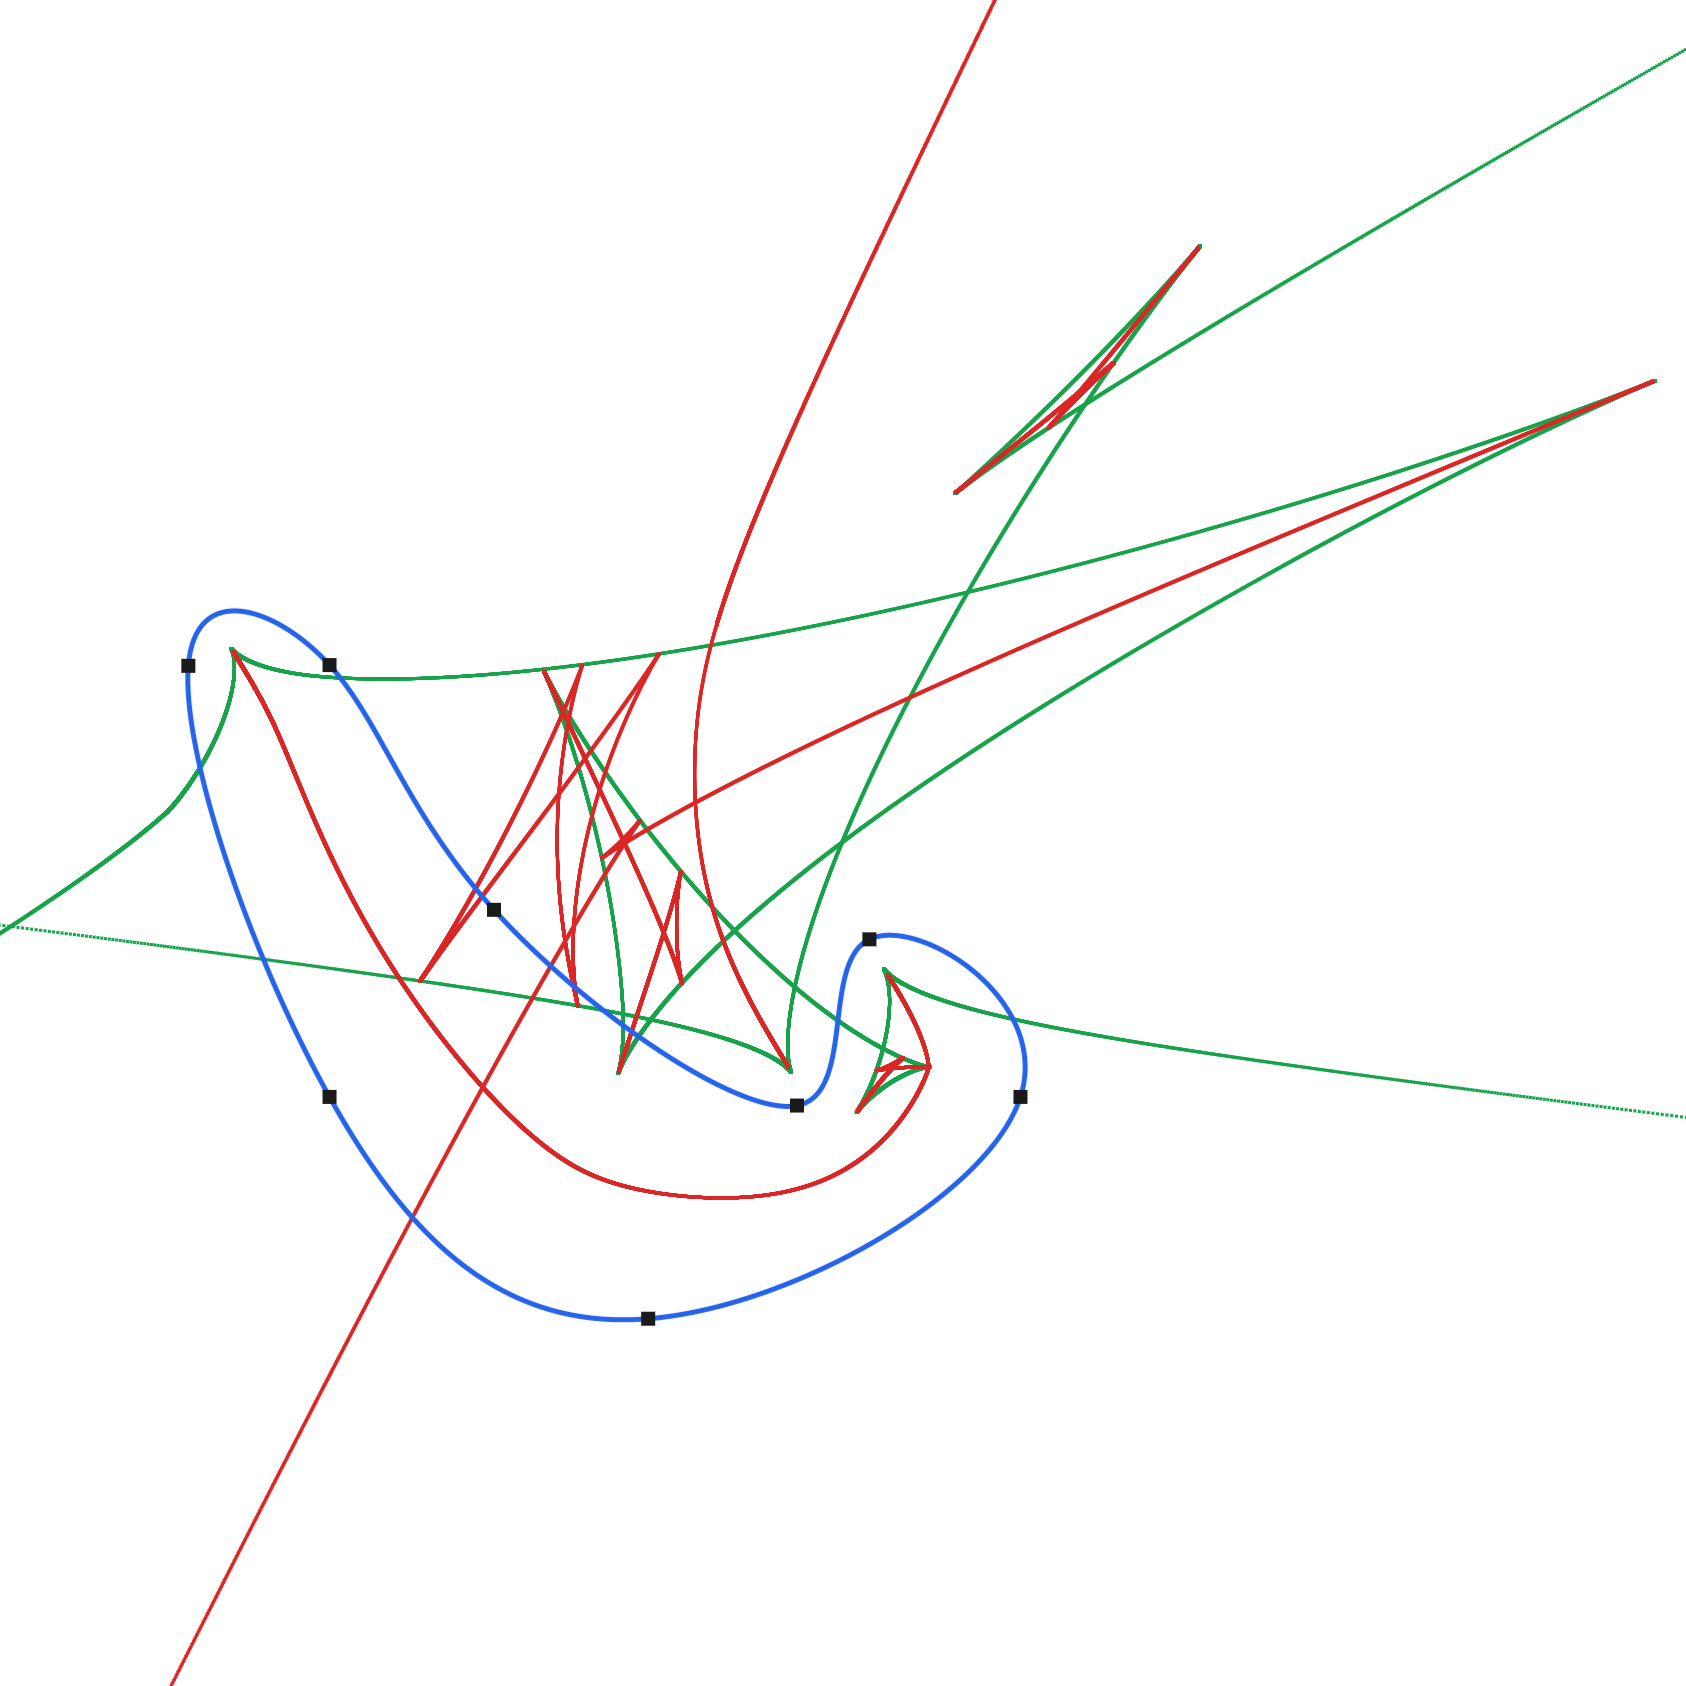
\includegraphics[width=0.42\linewidth]{fun1.png}
        \hfill
        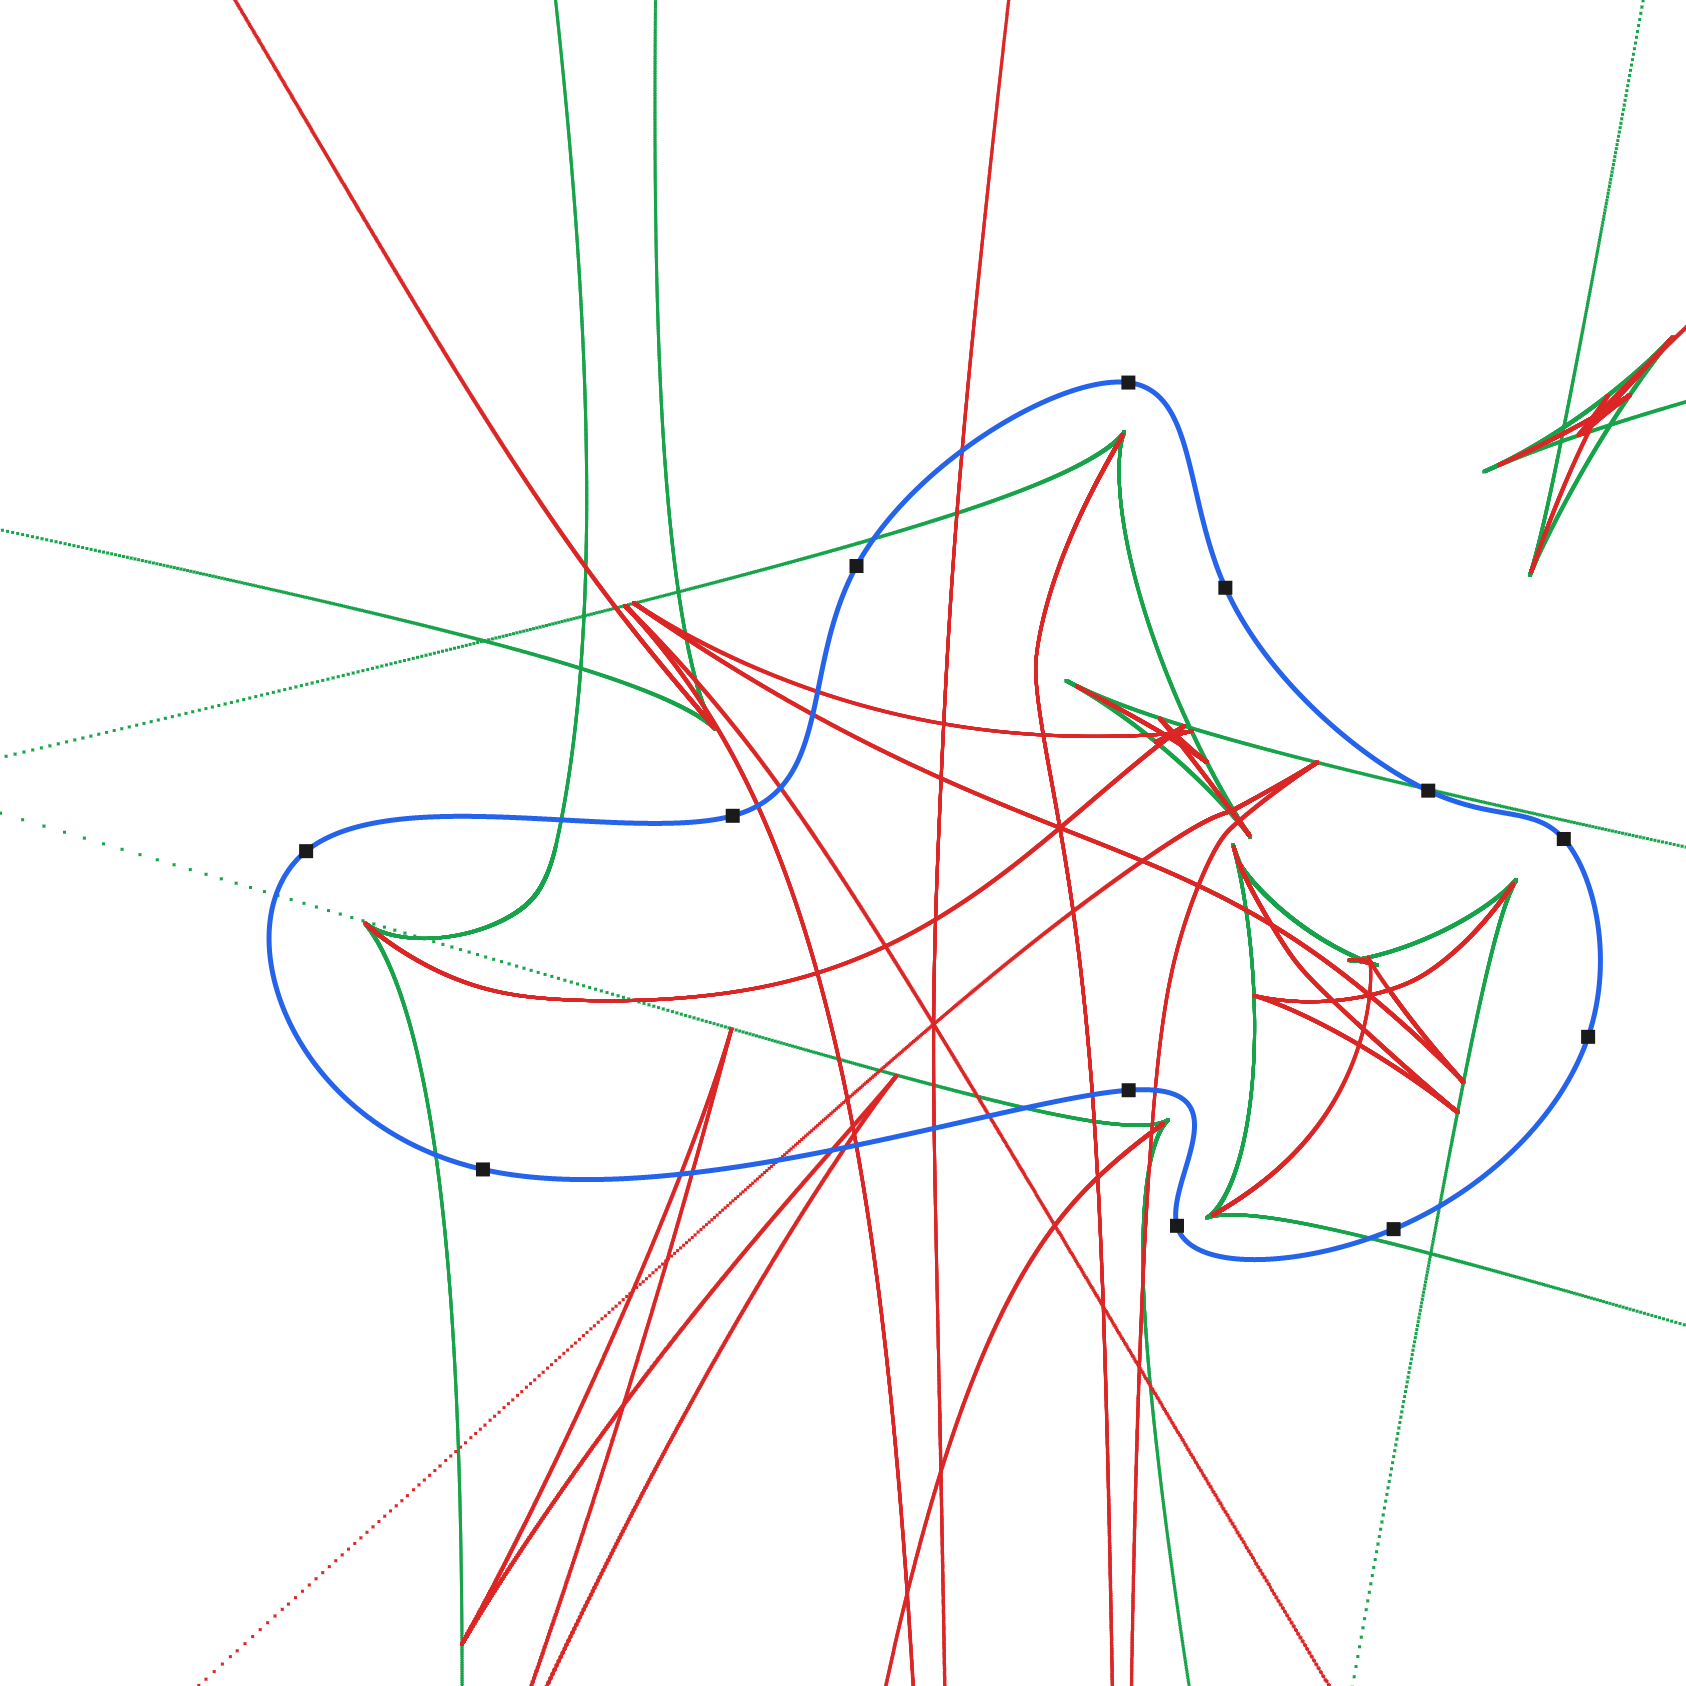
\includegraphics[width=0.42\linewidth]{fun2.png}

        \vspace{0.3em}

        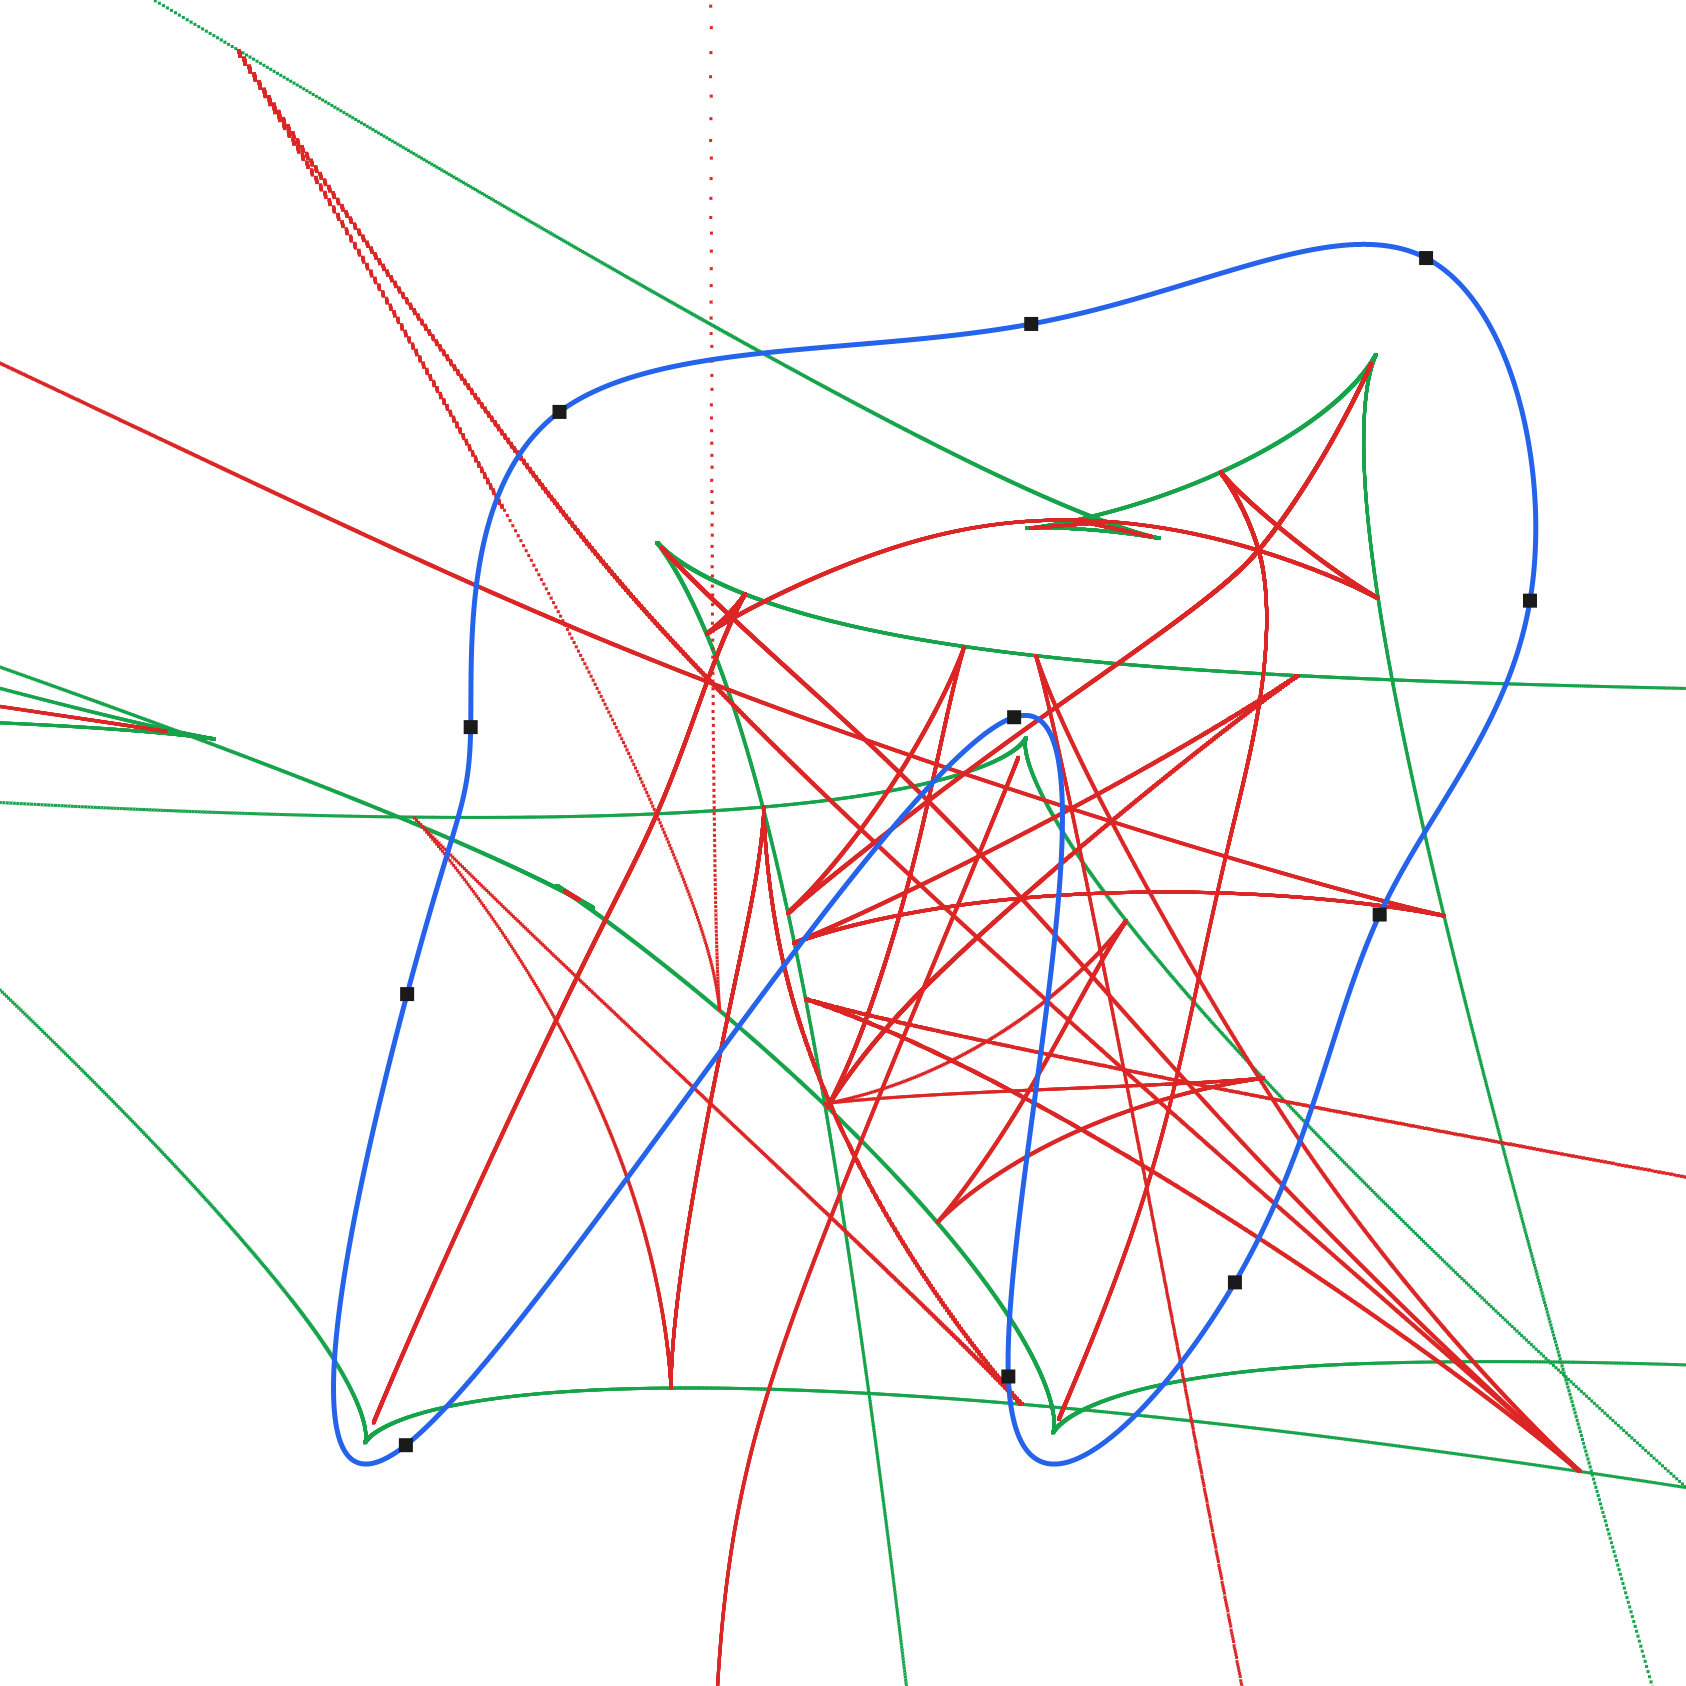
\includegraphics[width=0.42\linewidth]{fun3.png}
        \hfill
        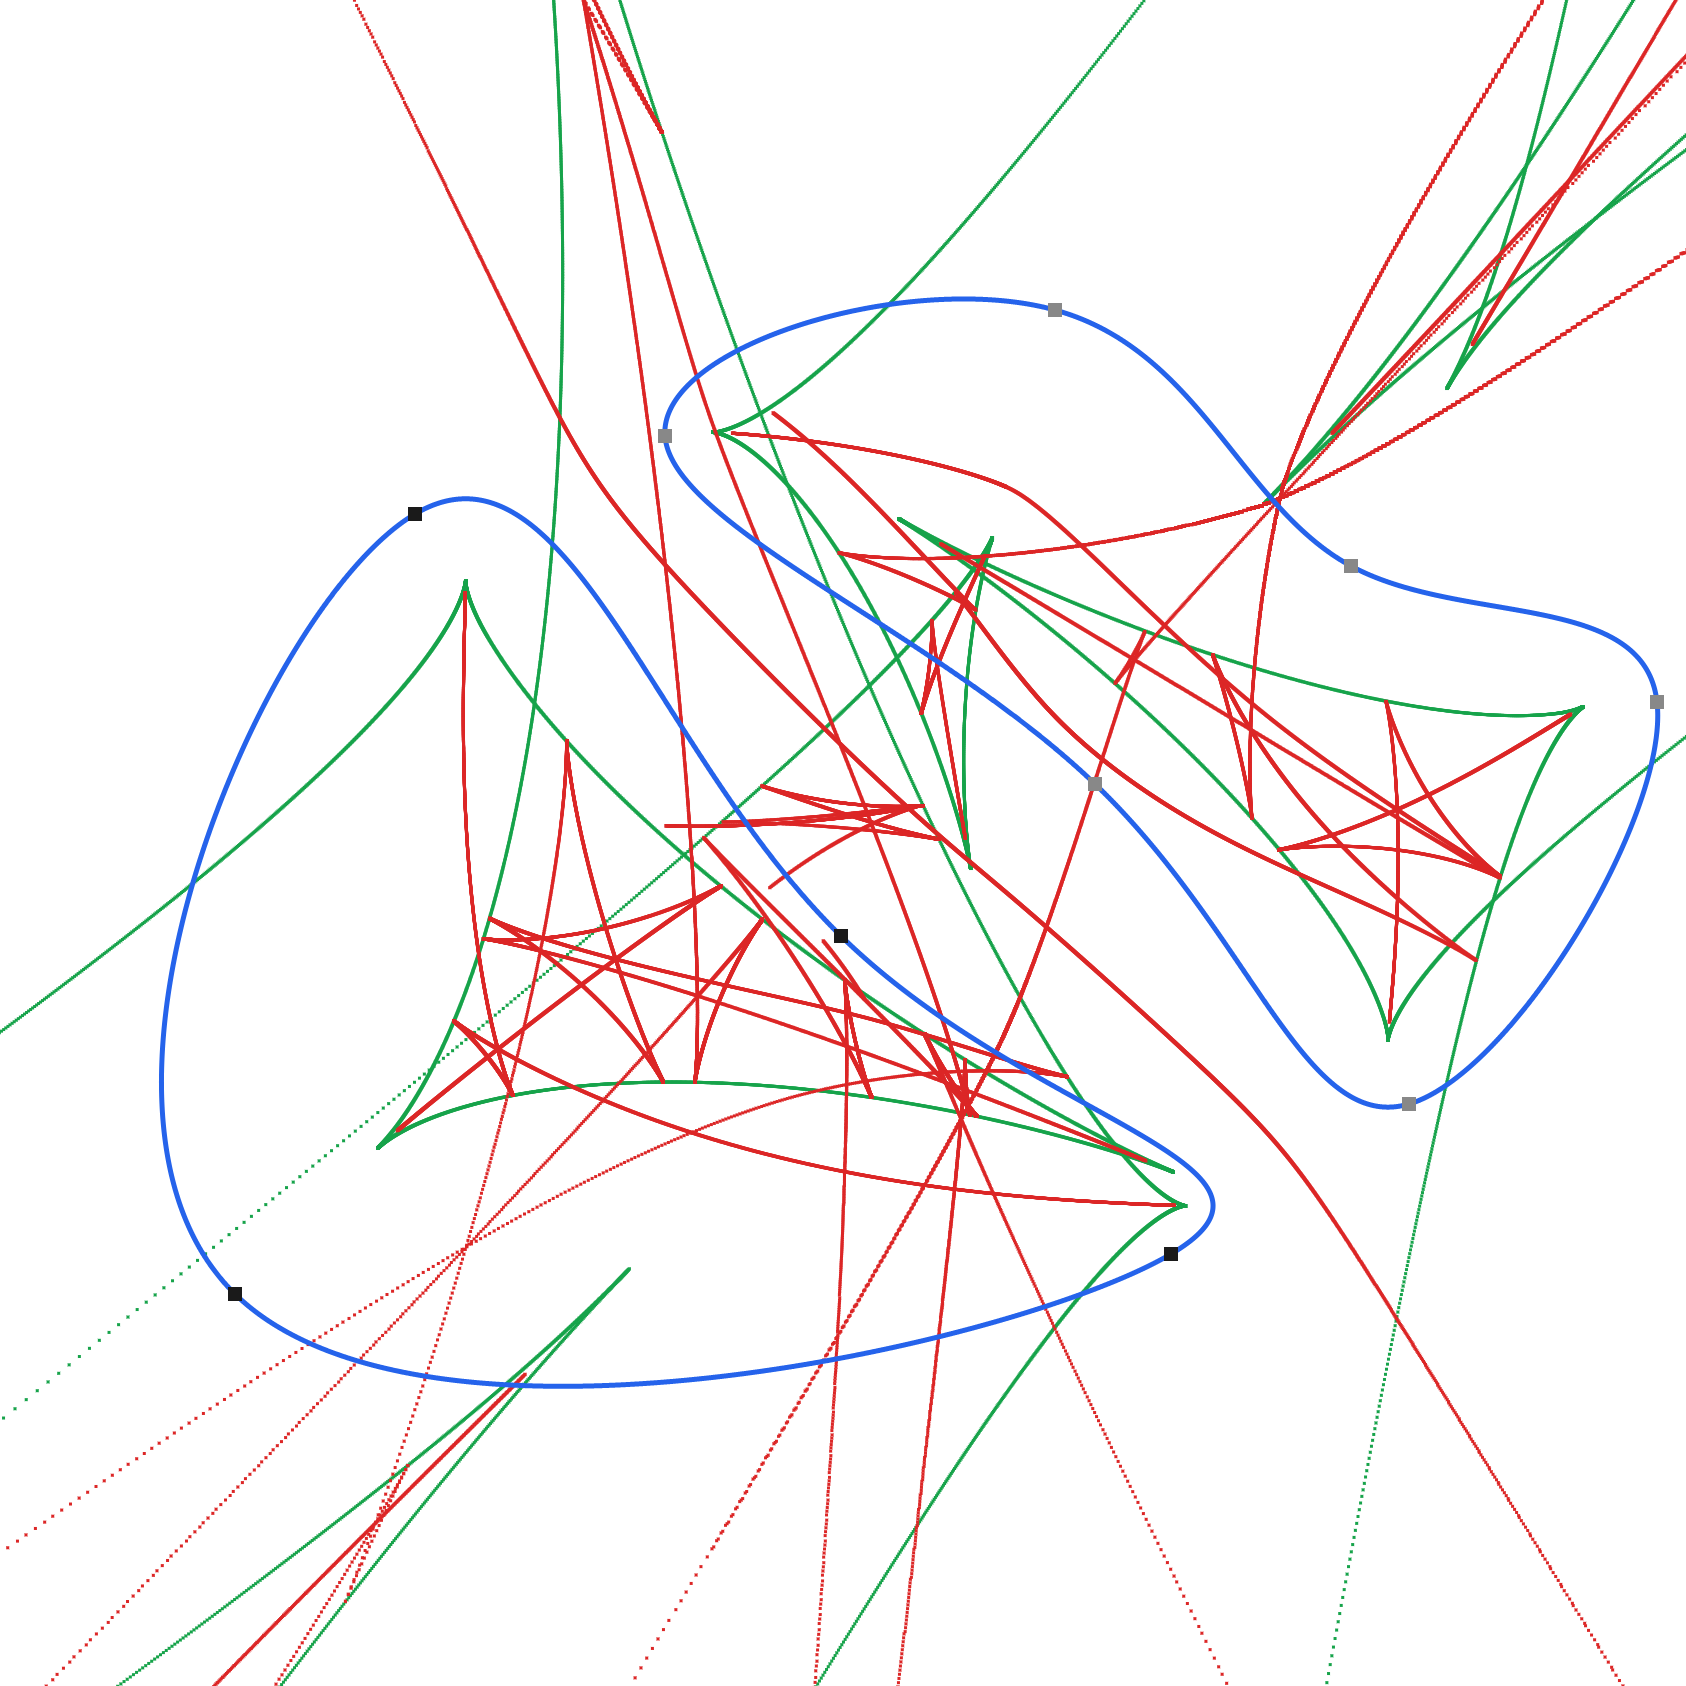
\includegraphics[width=0.42\linewidth]{2_components.png}
        \caption{Complex symmetry/focal sets. Bottom right: two disjoint components showing inter-component bitangential interactions.}
    \end{figure}
\end{frame}

\begin{frame}{Vineyard: Crossing the Focal Set}
    Topological changes occur precisely when $\gamma(t)$ crosses the focal set:
    \begin{figure}
        \centering
        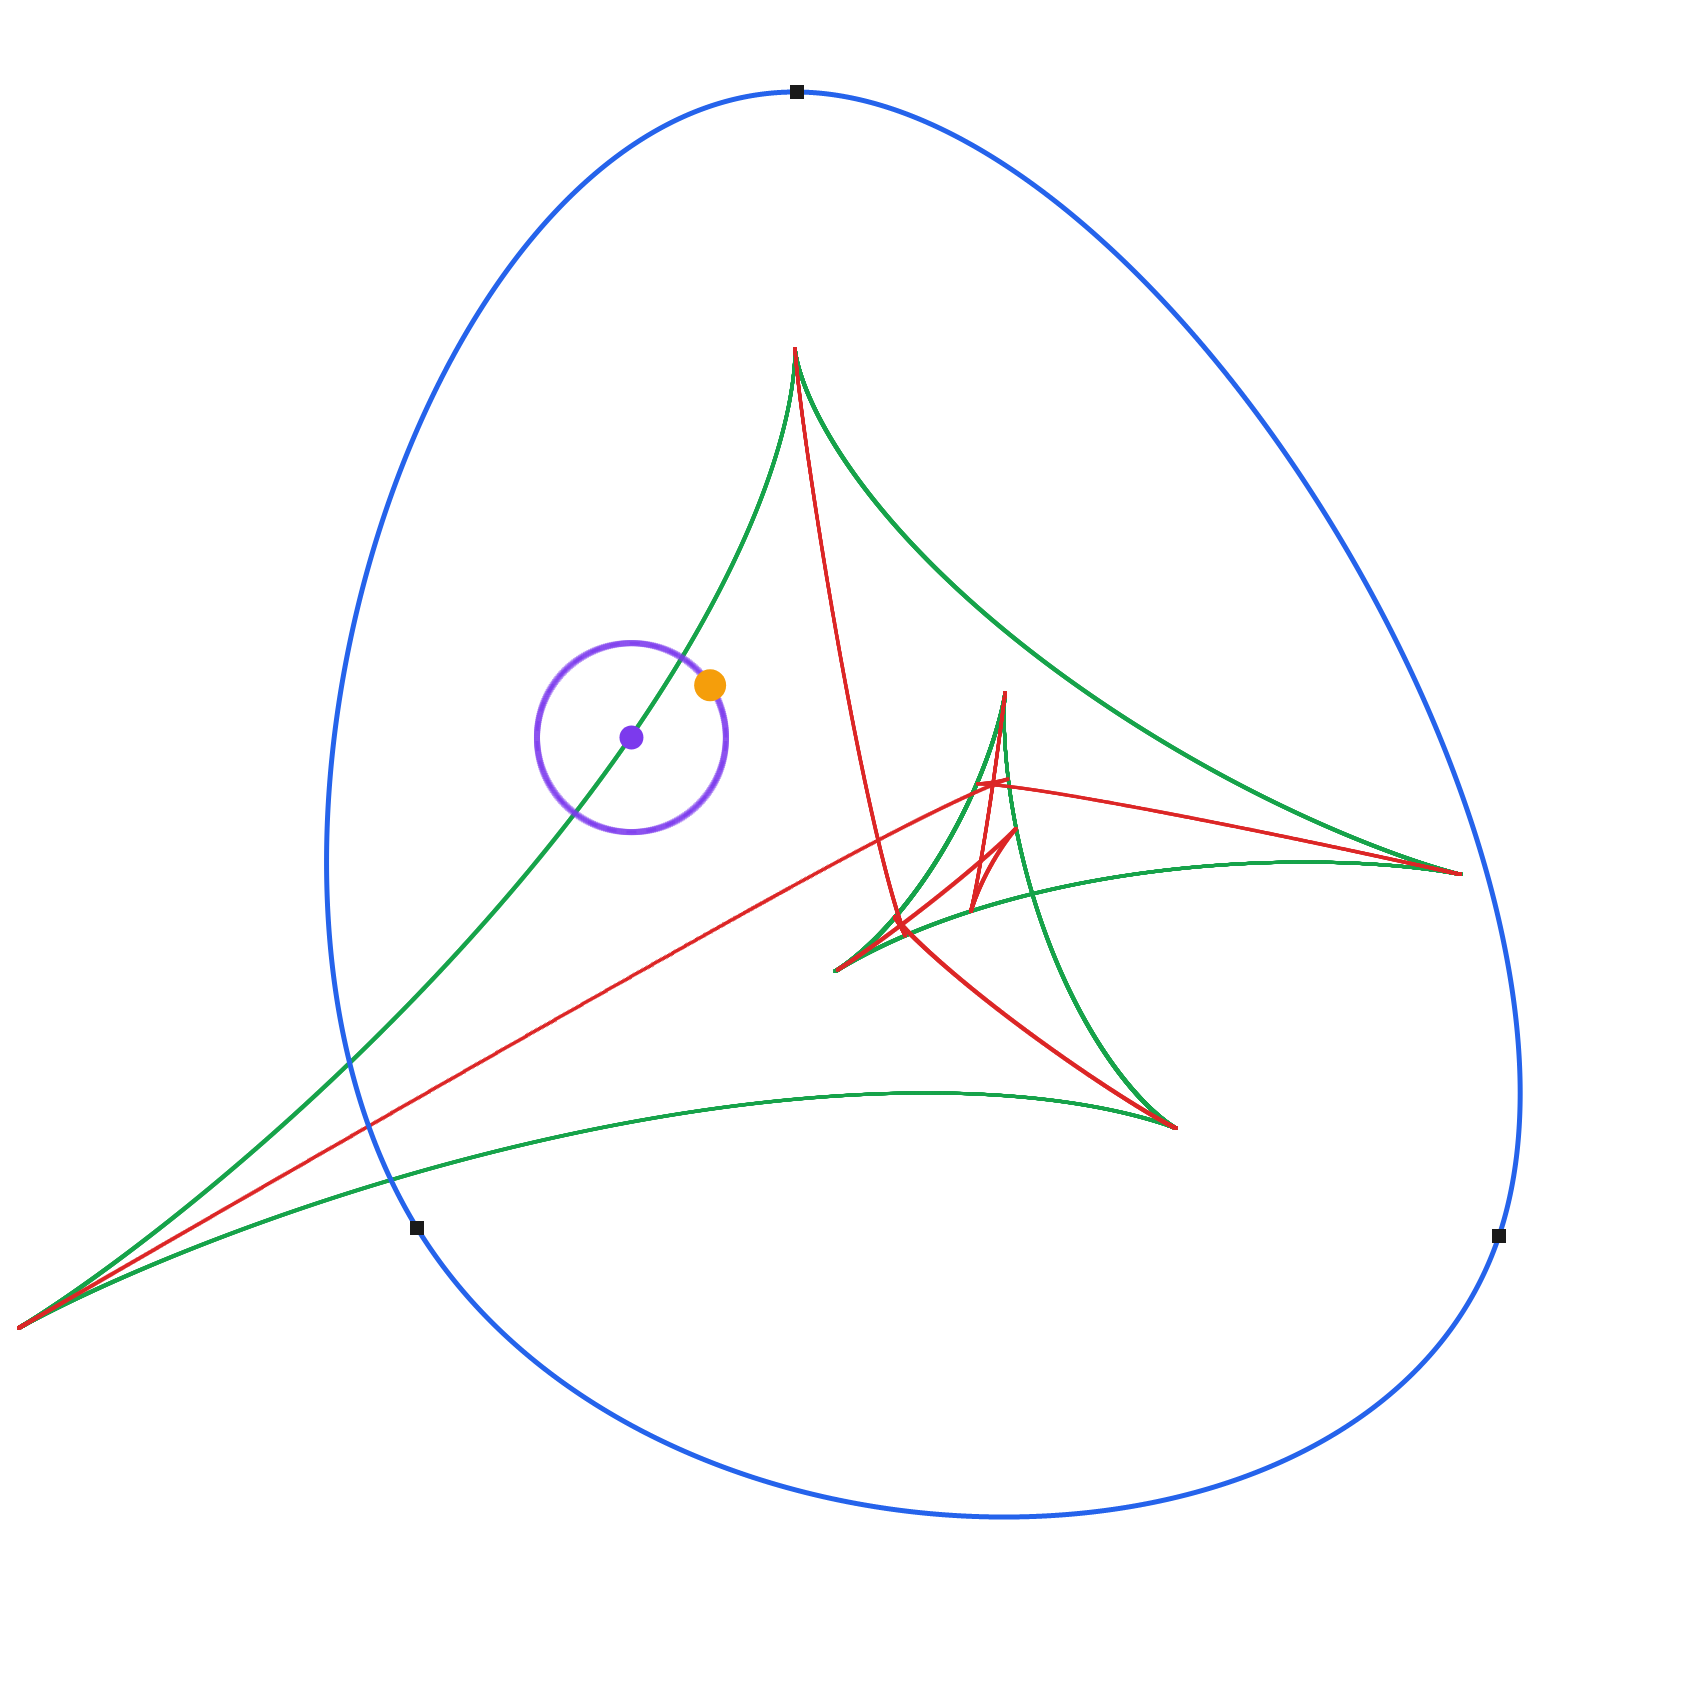
\includegraphics[width=0.30\textwidth]{canvas1.png}
        \hfill
        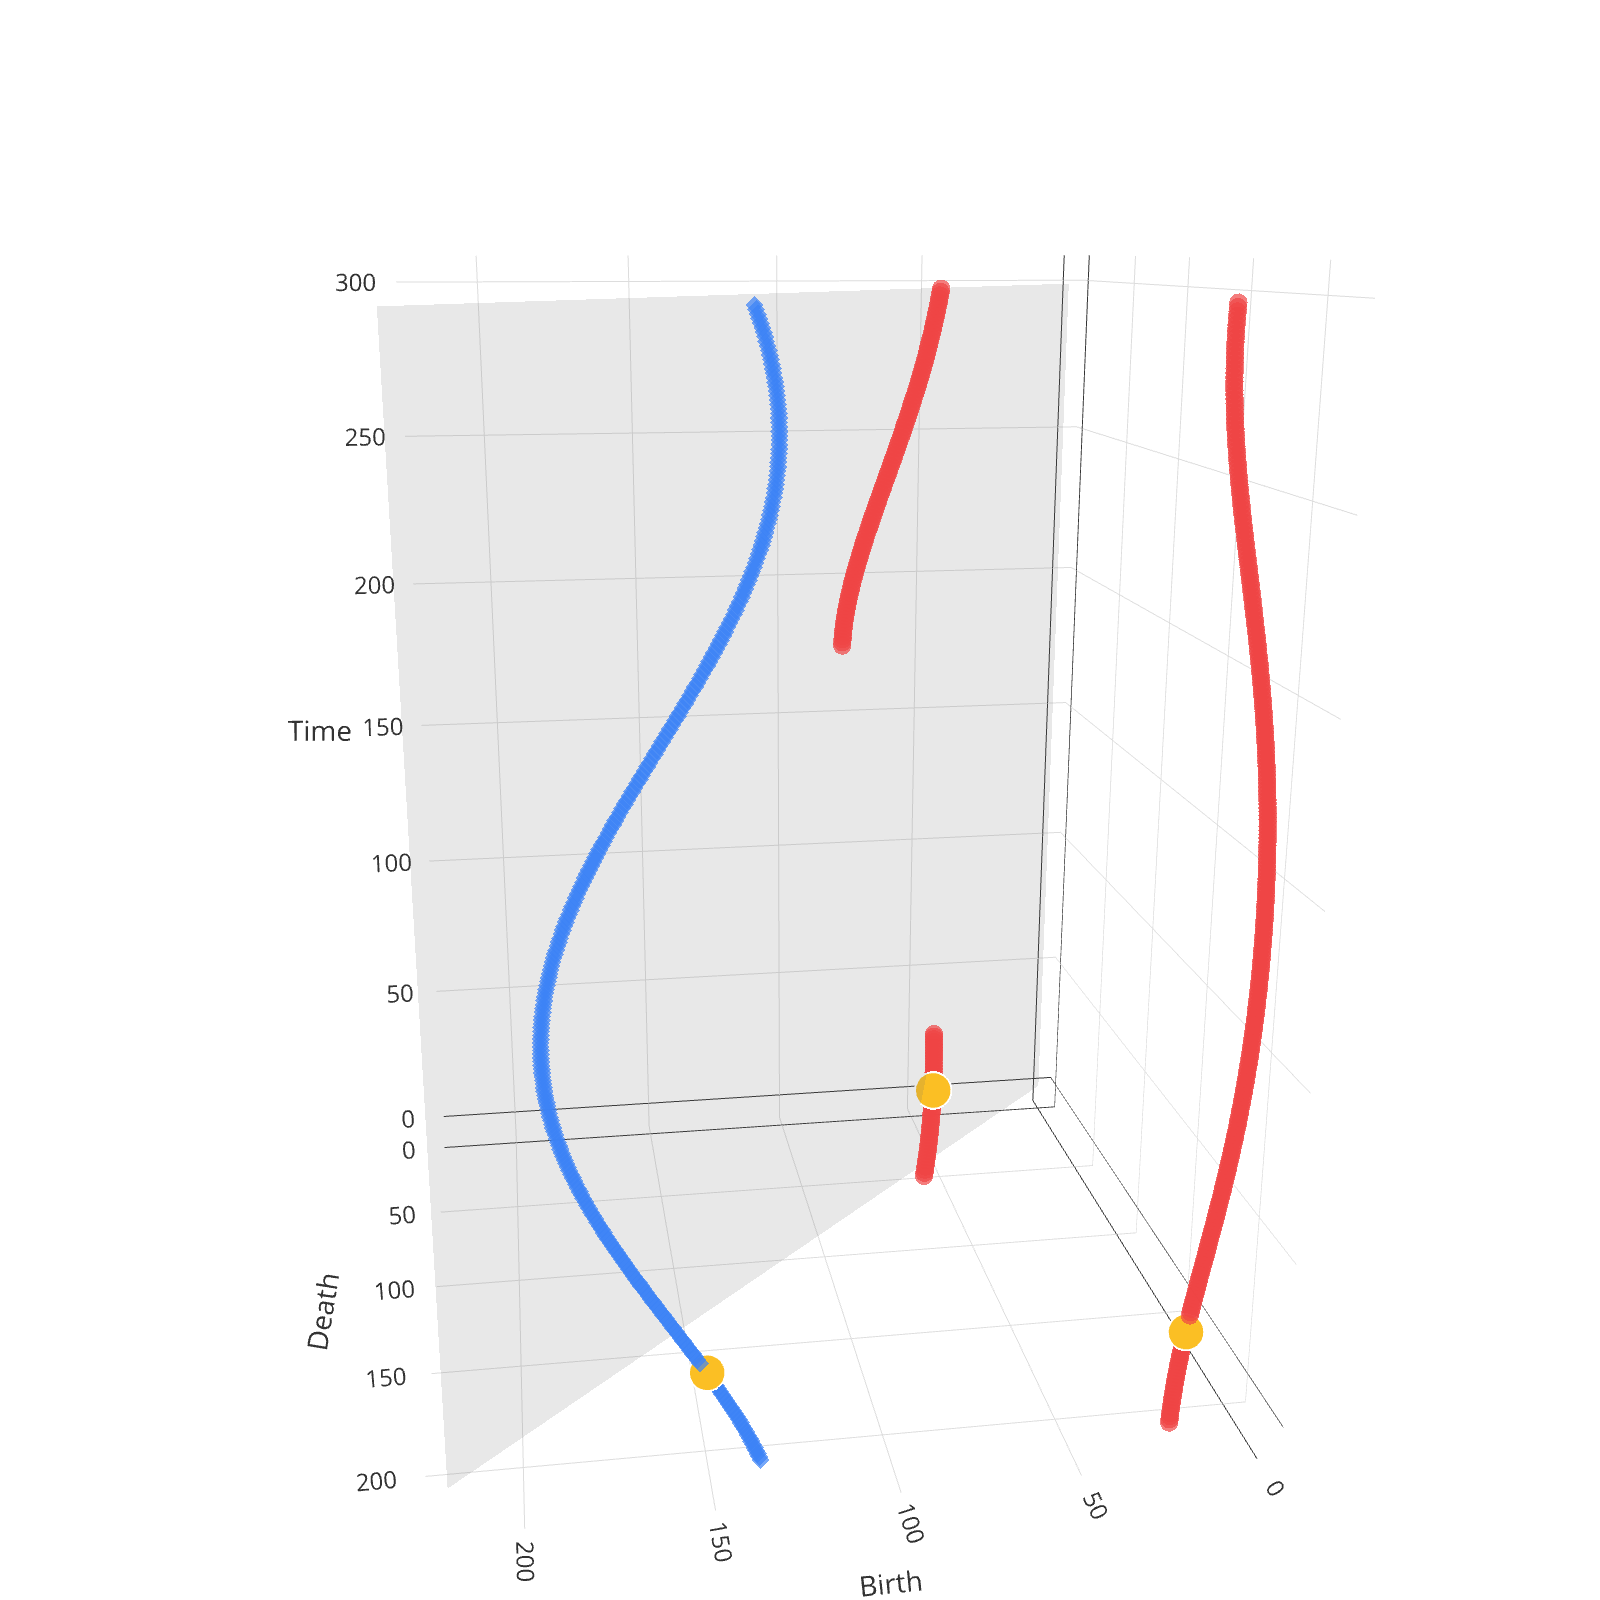
\includegraphics[width=0.34\textwidth]{vin1.png}
        \hfill
        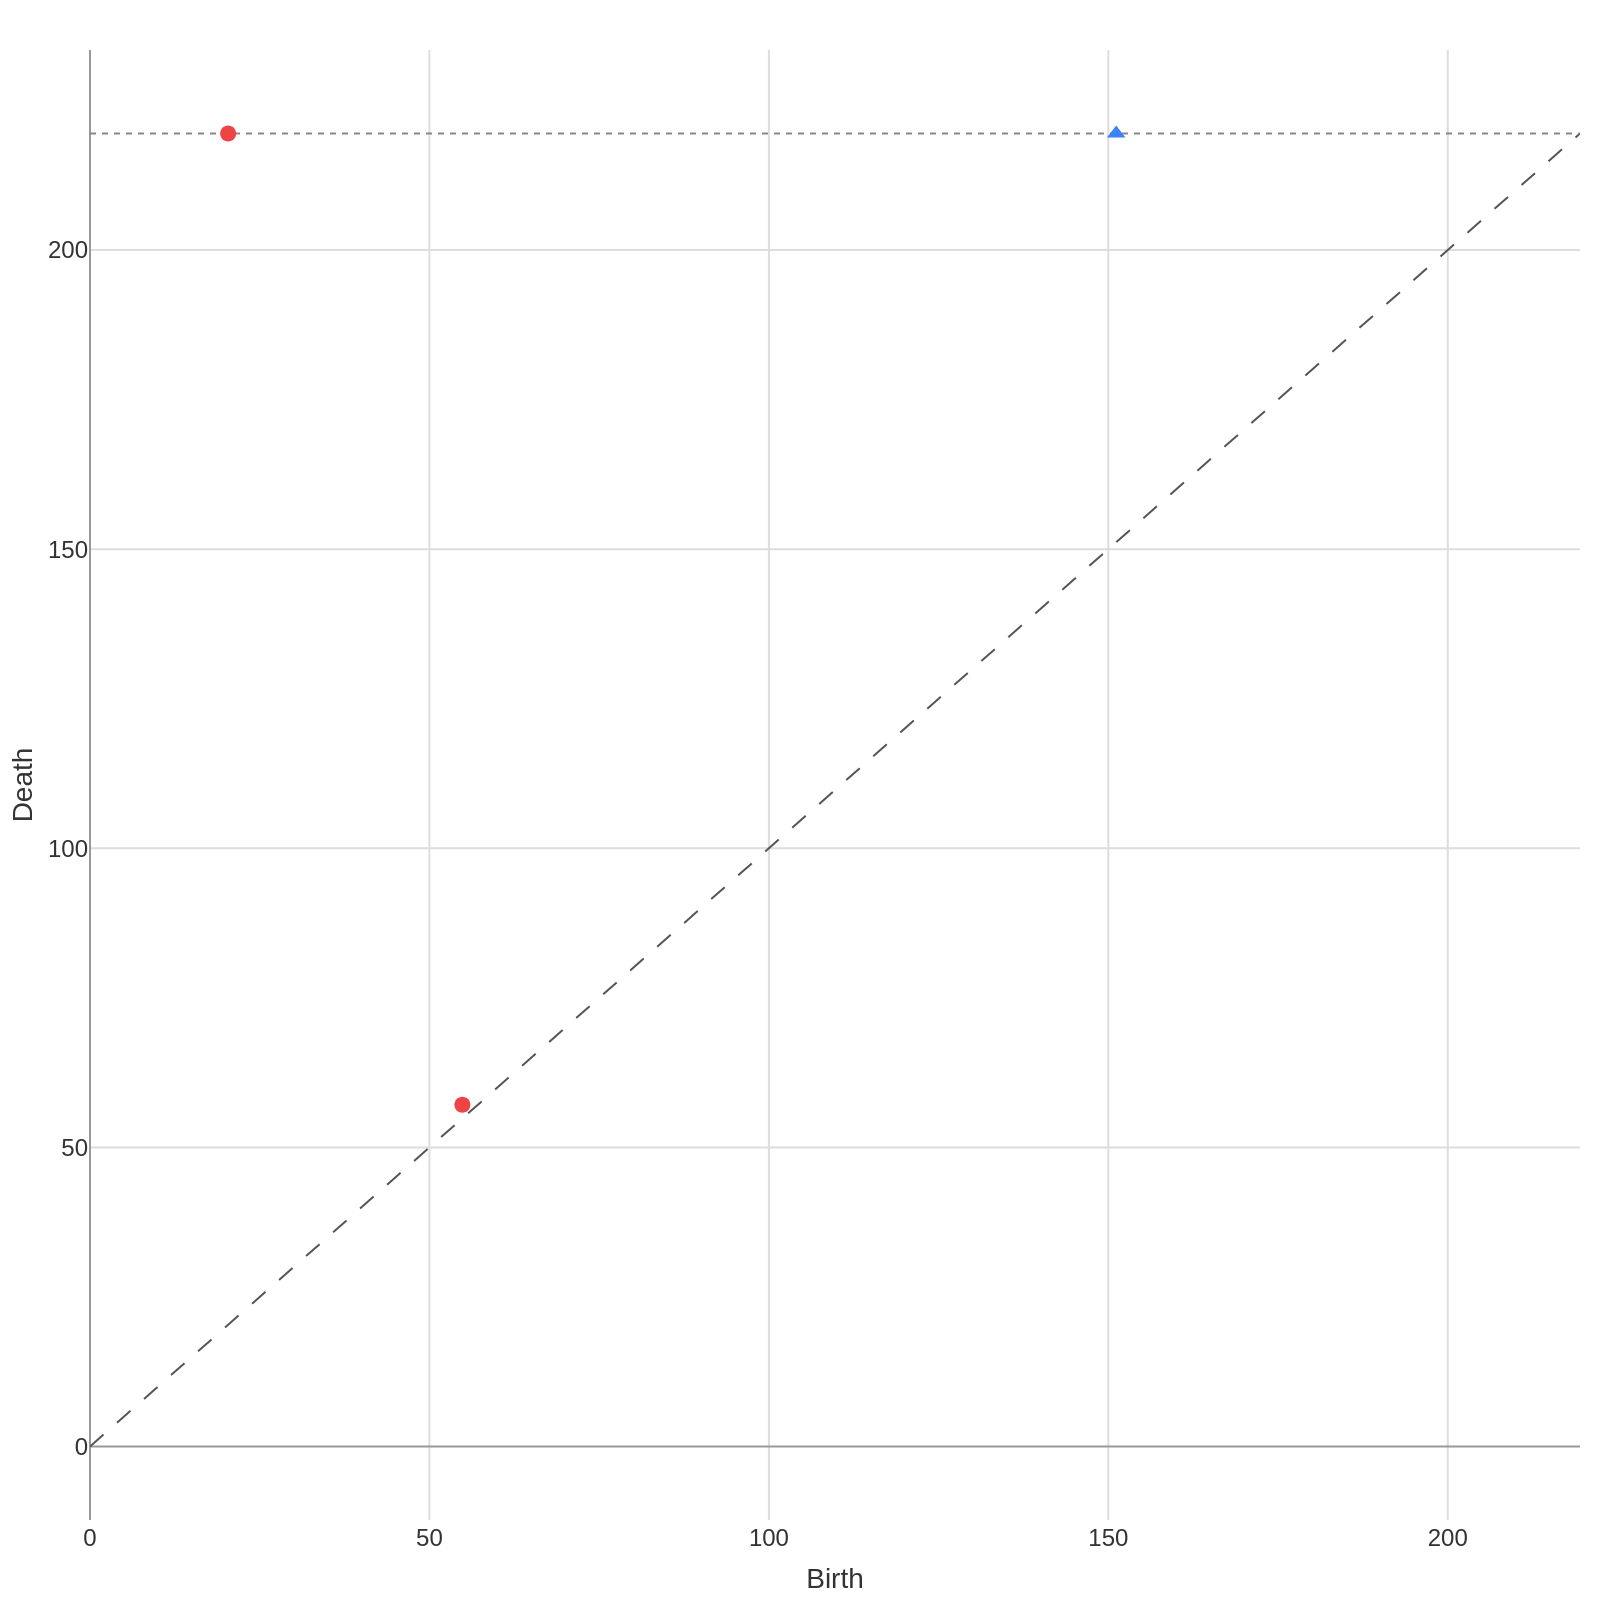
\includegraphics[width=0.27\textwidth]{persistence_diagram1.png}

        \vspace{0.2em}

        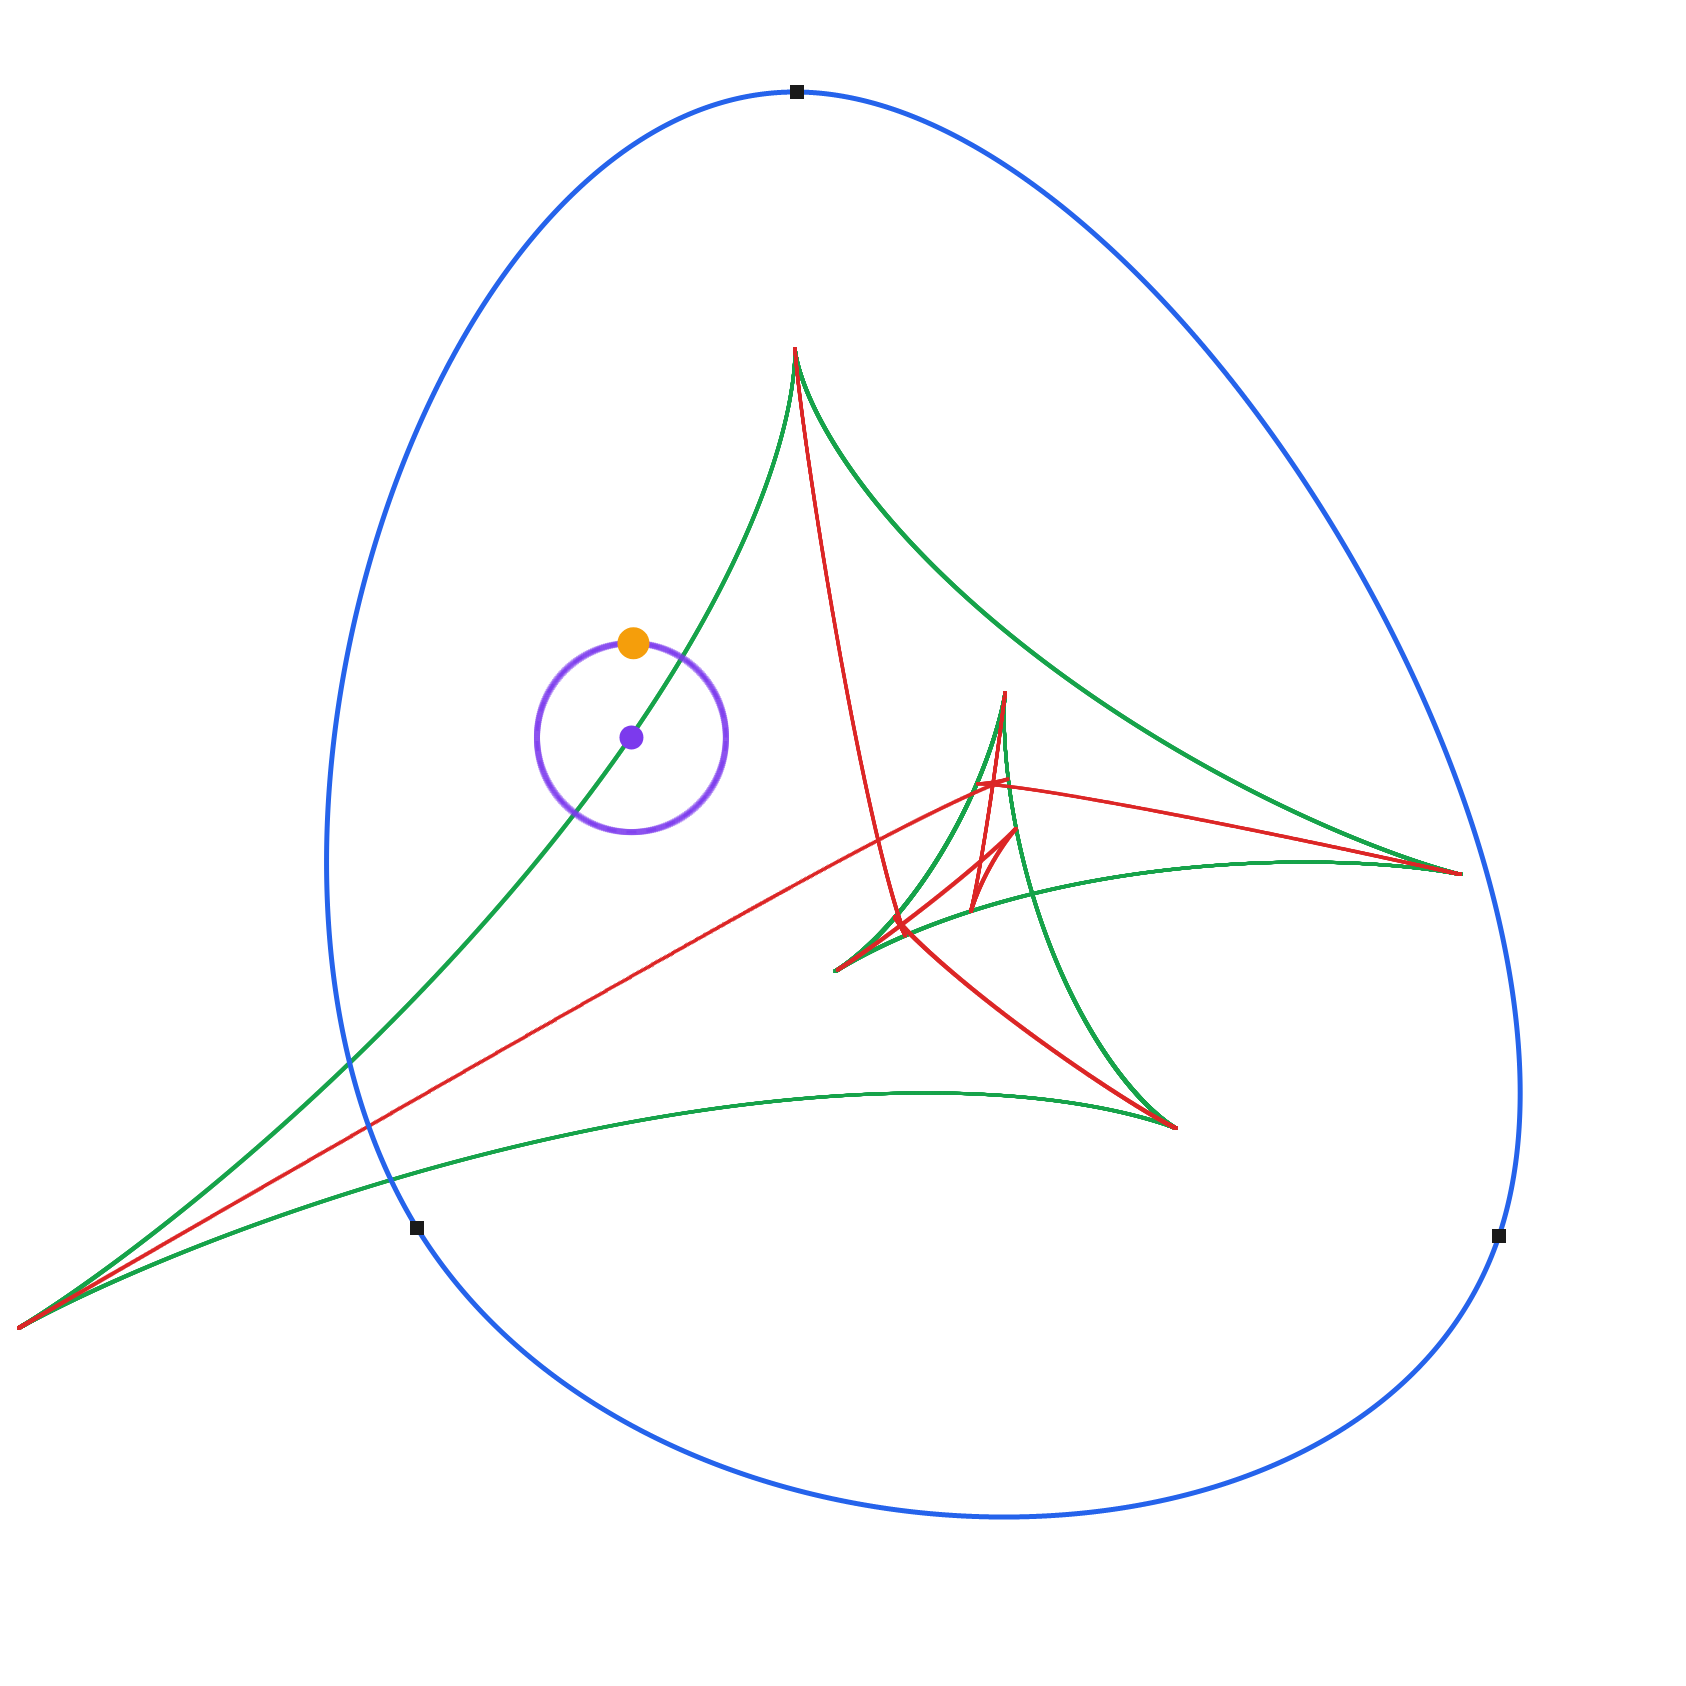
\includegraphics[width=0.30\textwidth]{canvas2.png}
        \hfill
        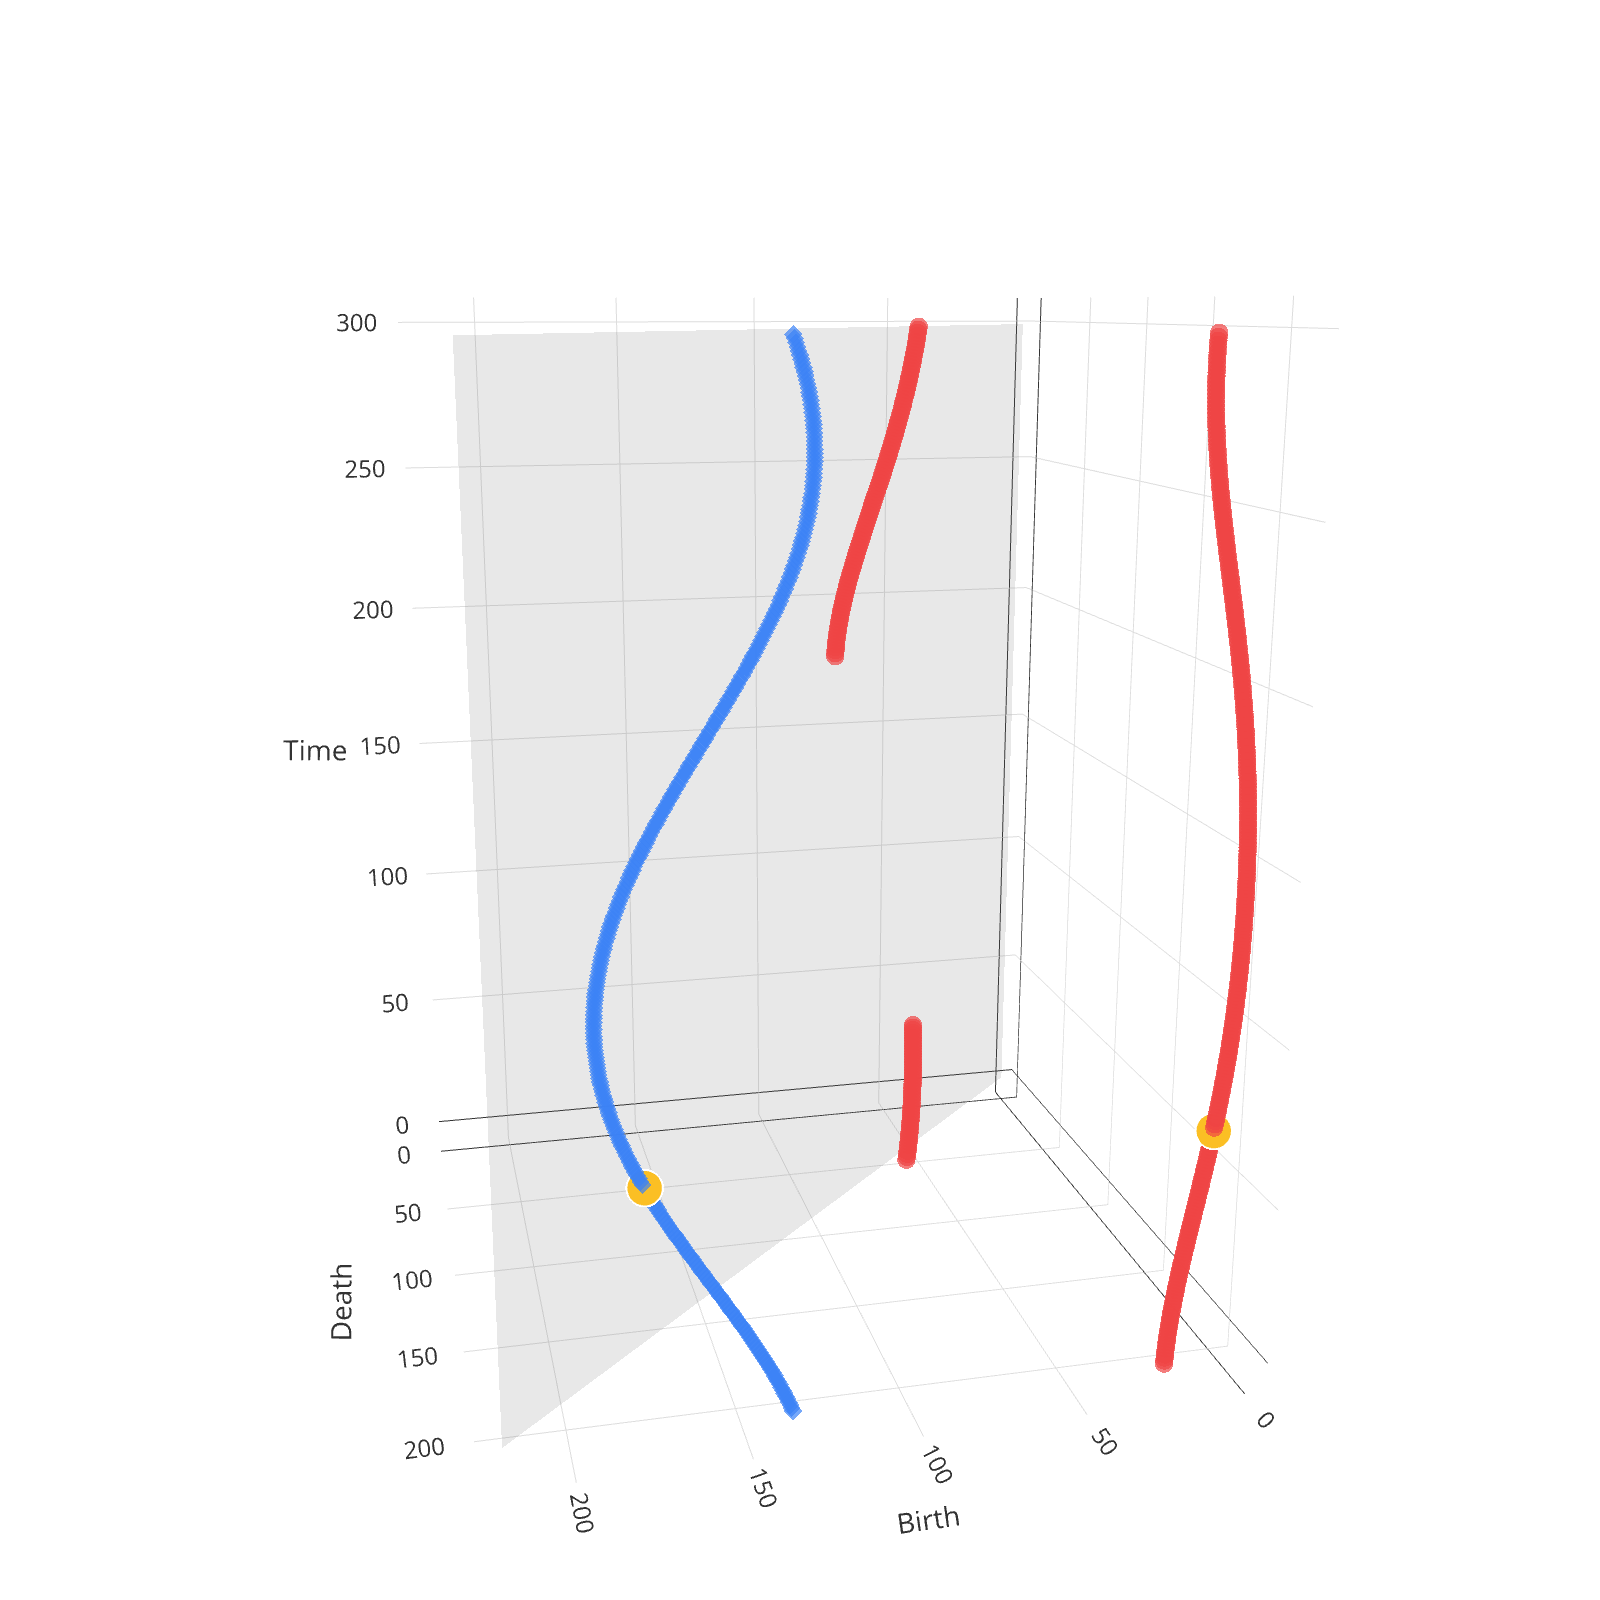
\includegraphics[width=0.34\textwidth]{vin2.png}
        \hfill
        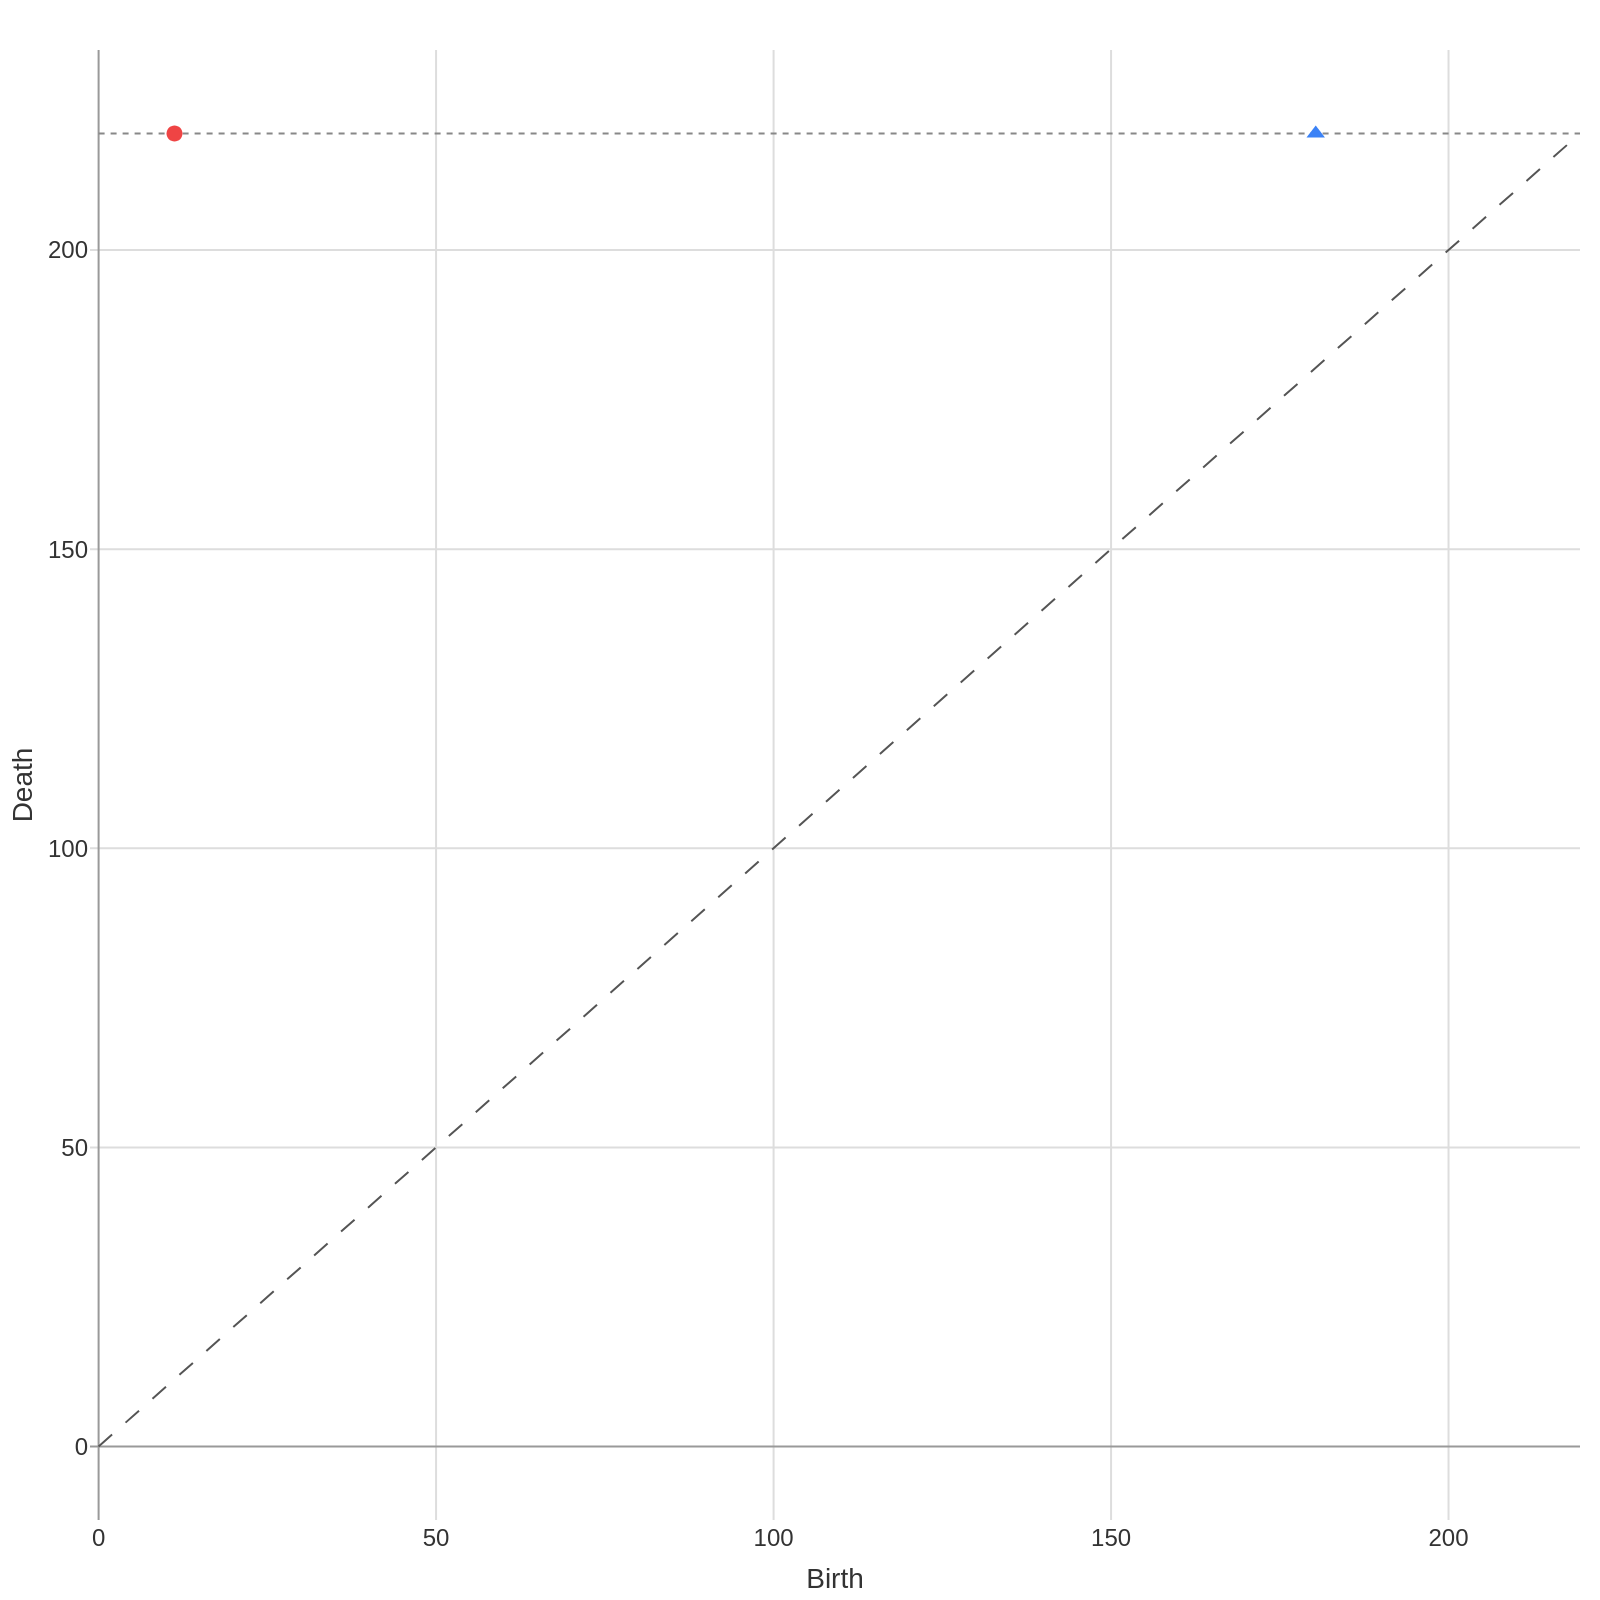
\includegraphics[width=0.27\textwidth]{persistence_diagram2.png}
        \caption{Top: center avoids focal set $\Rightarrow$ continuous vine. Bottom: center crosses focal set $\Rightarrow$ break in the vineyard.}
    \end{figure}
\end{frame}

\begin{frame}{Vineyard: Crossing the Focal Set (cont.)}
    \begin{figure}
        \centering
        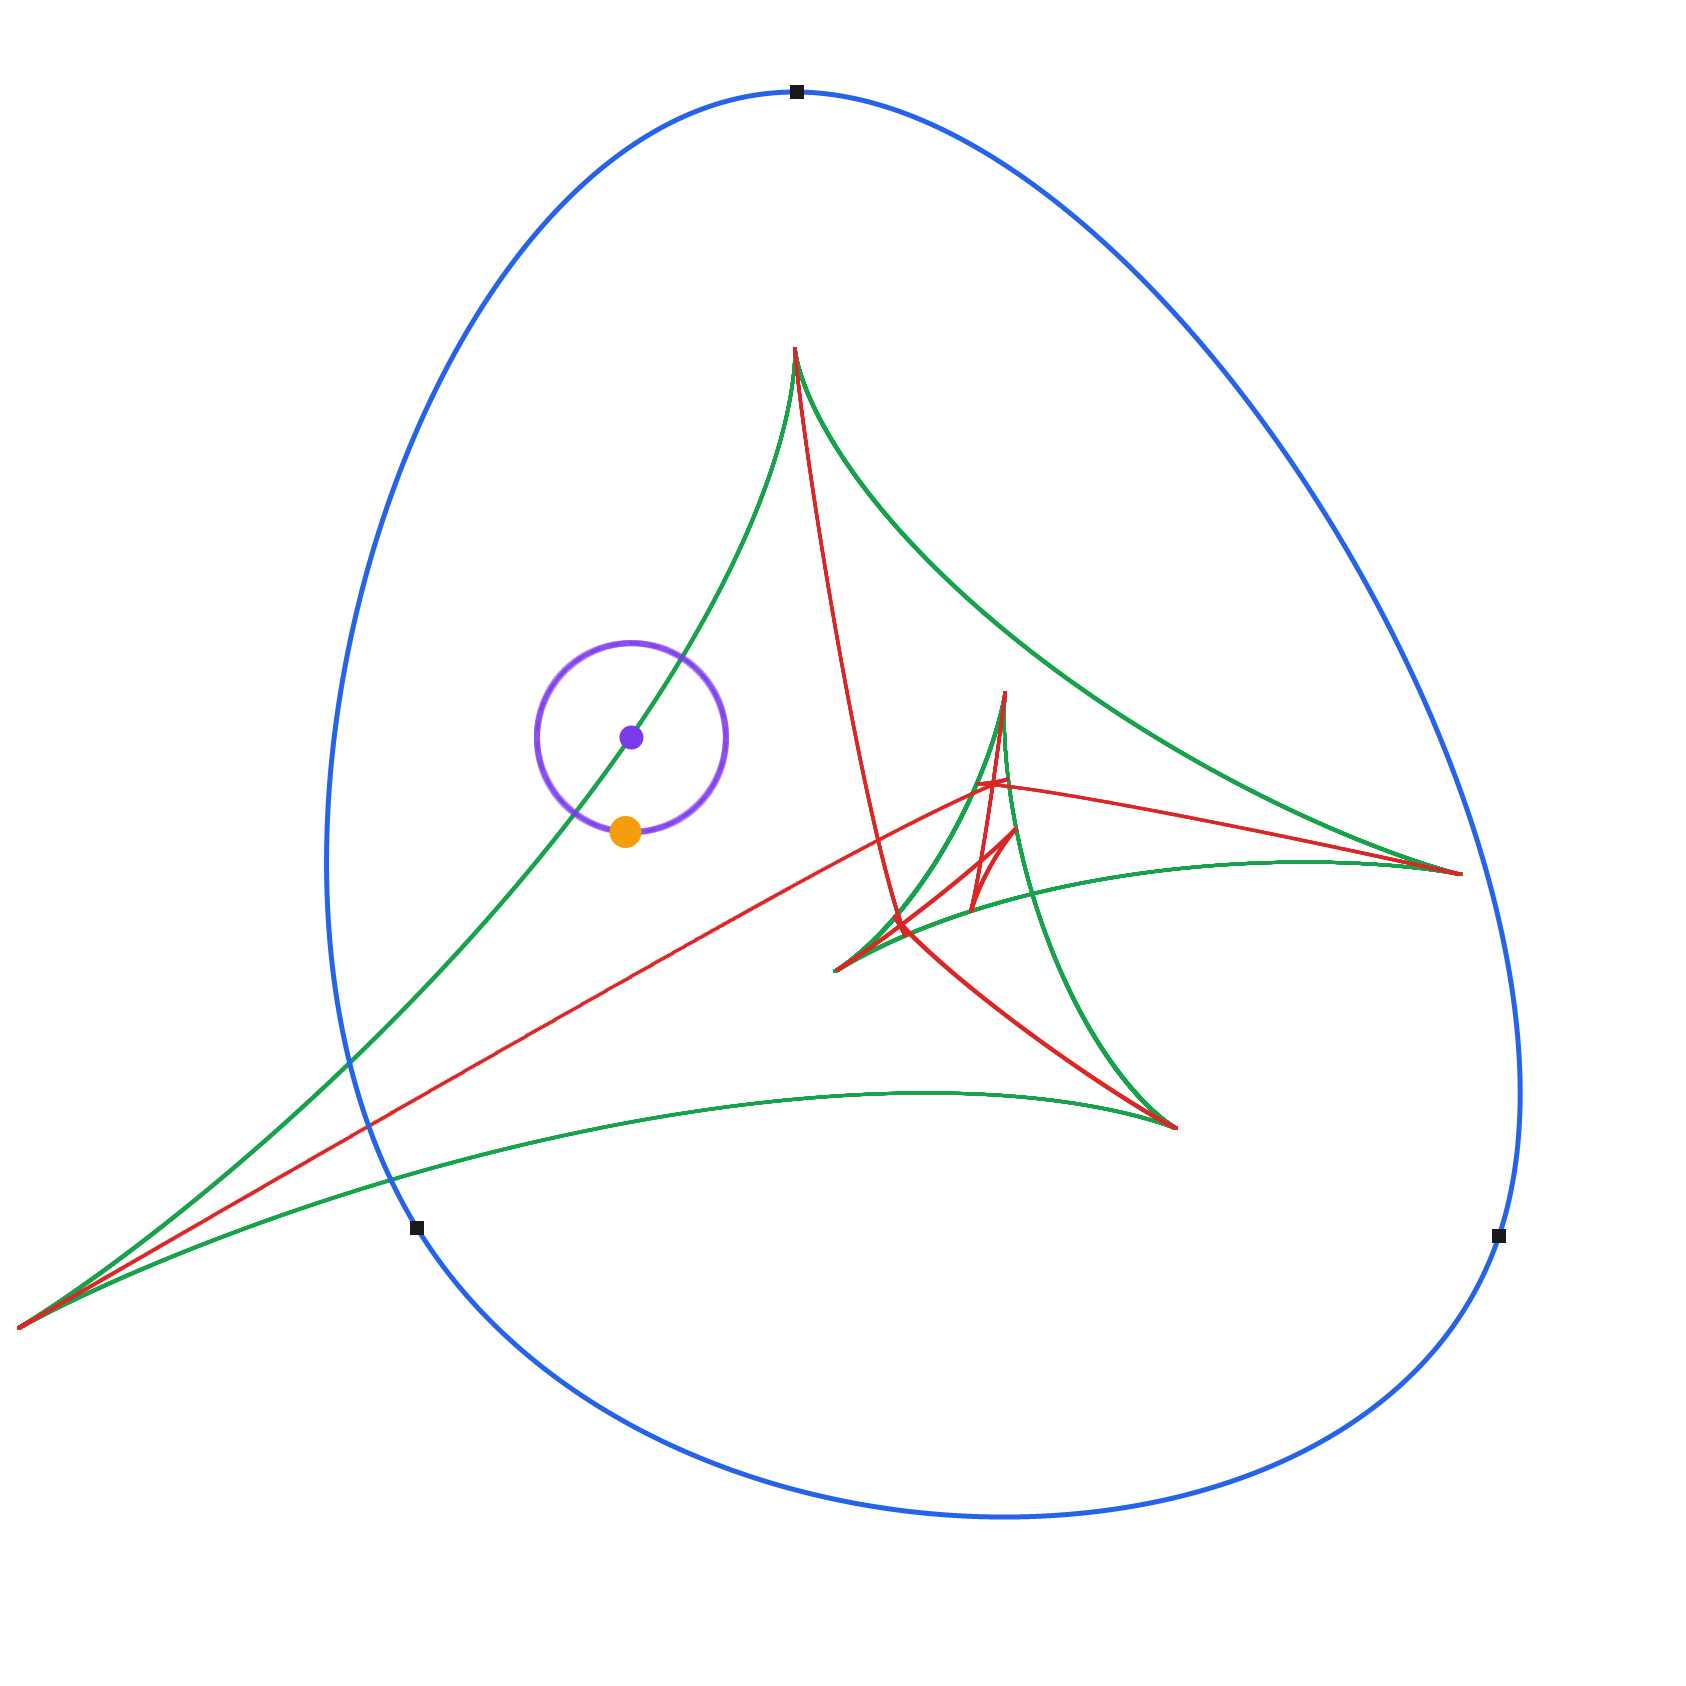
\includegraphics[width=0.30\textwidth]{canvas3.png}
        \hfill
        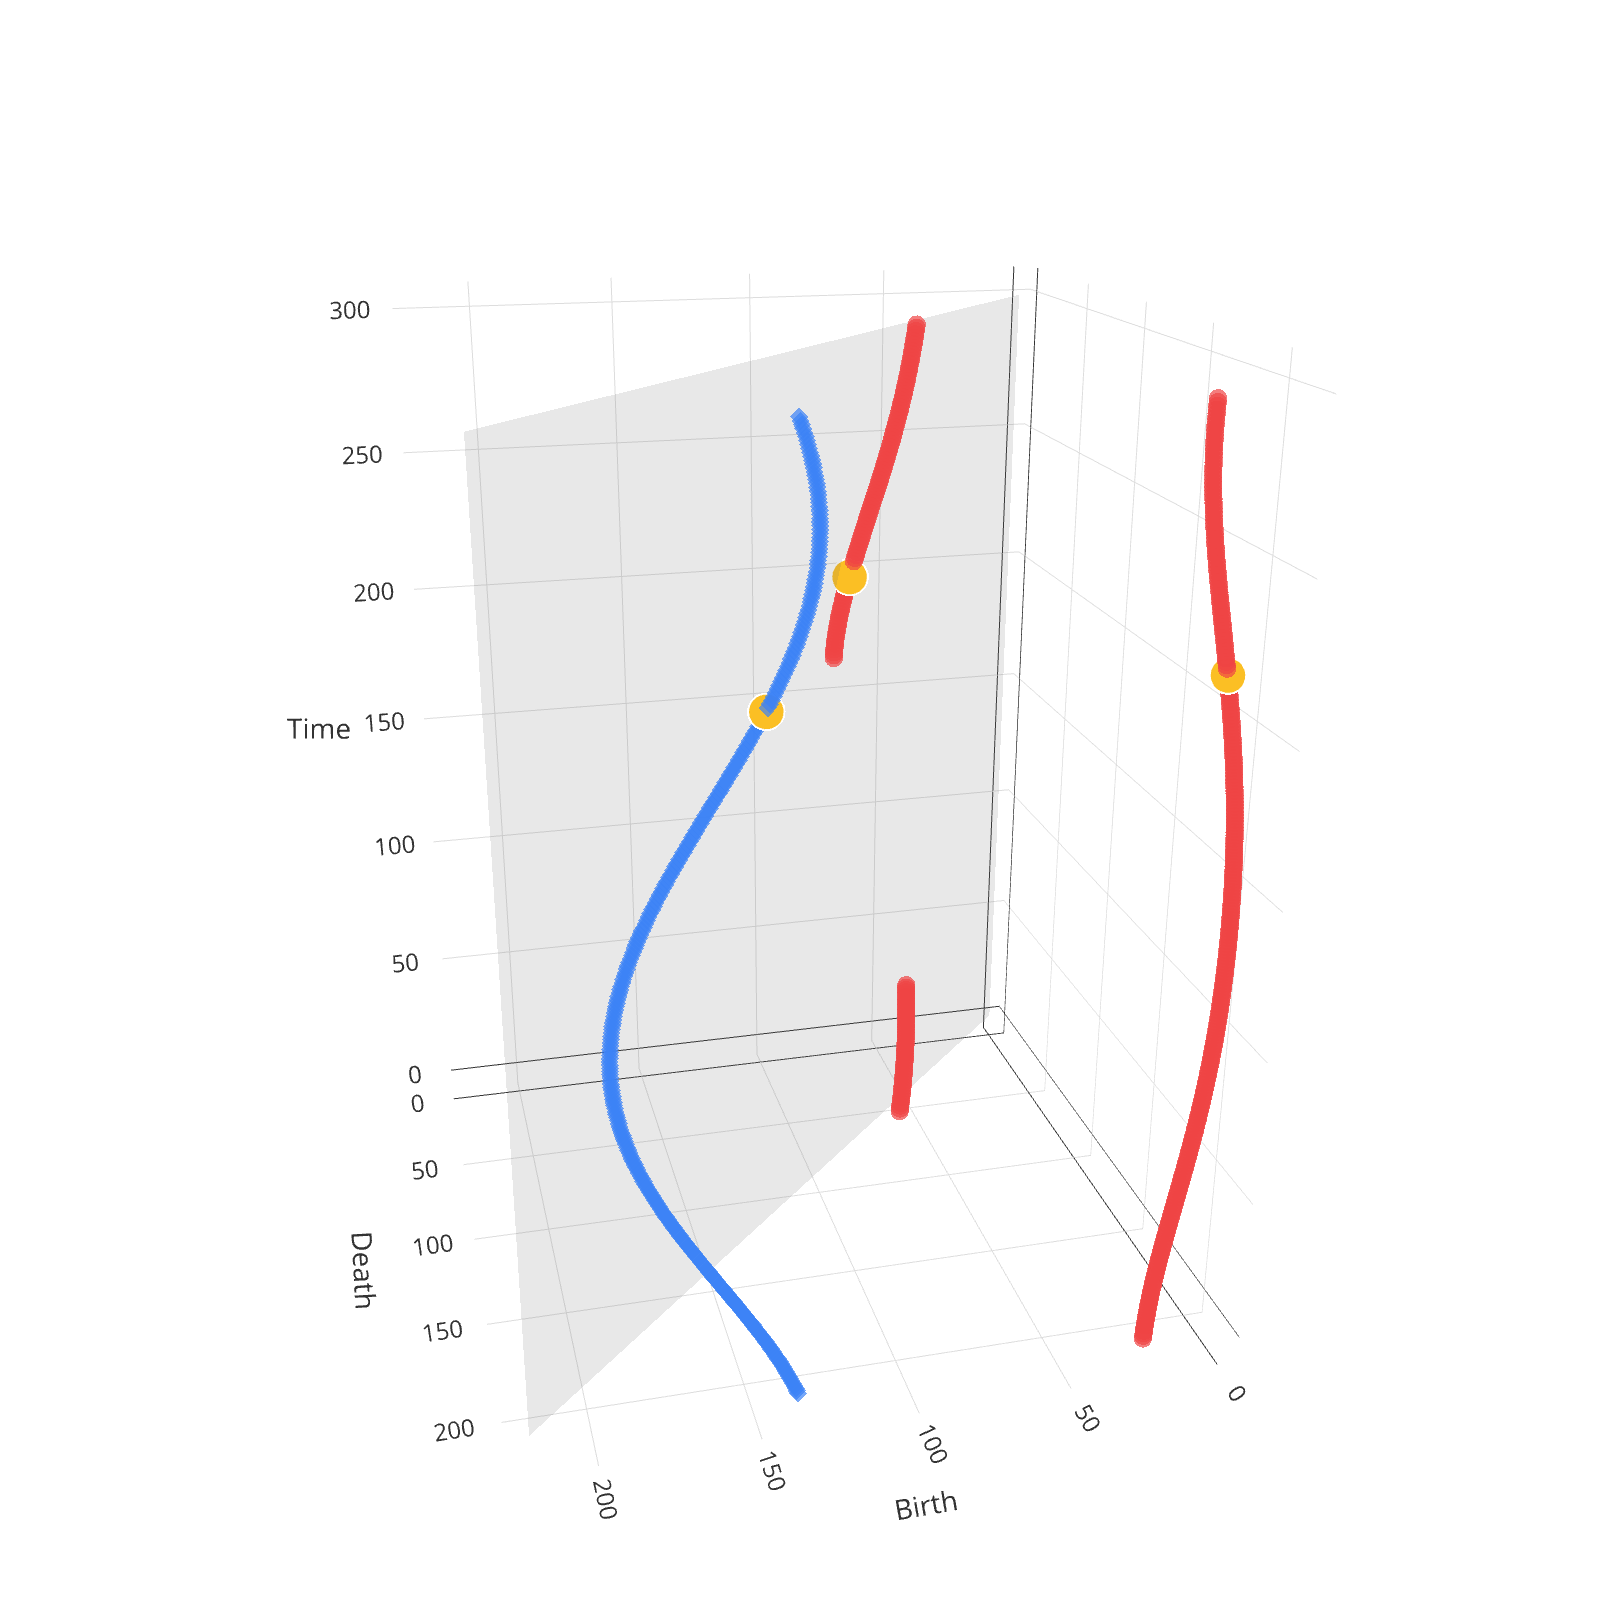
\includegraphics[width=0.34\textwidth]{vin3.png}
        \hfill
        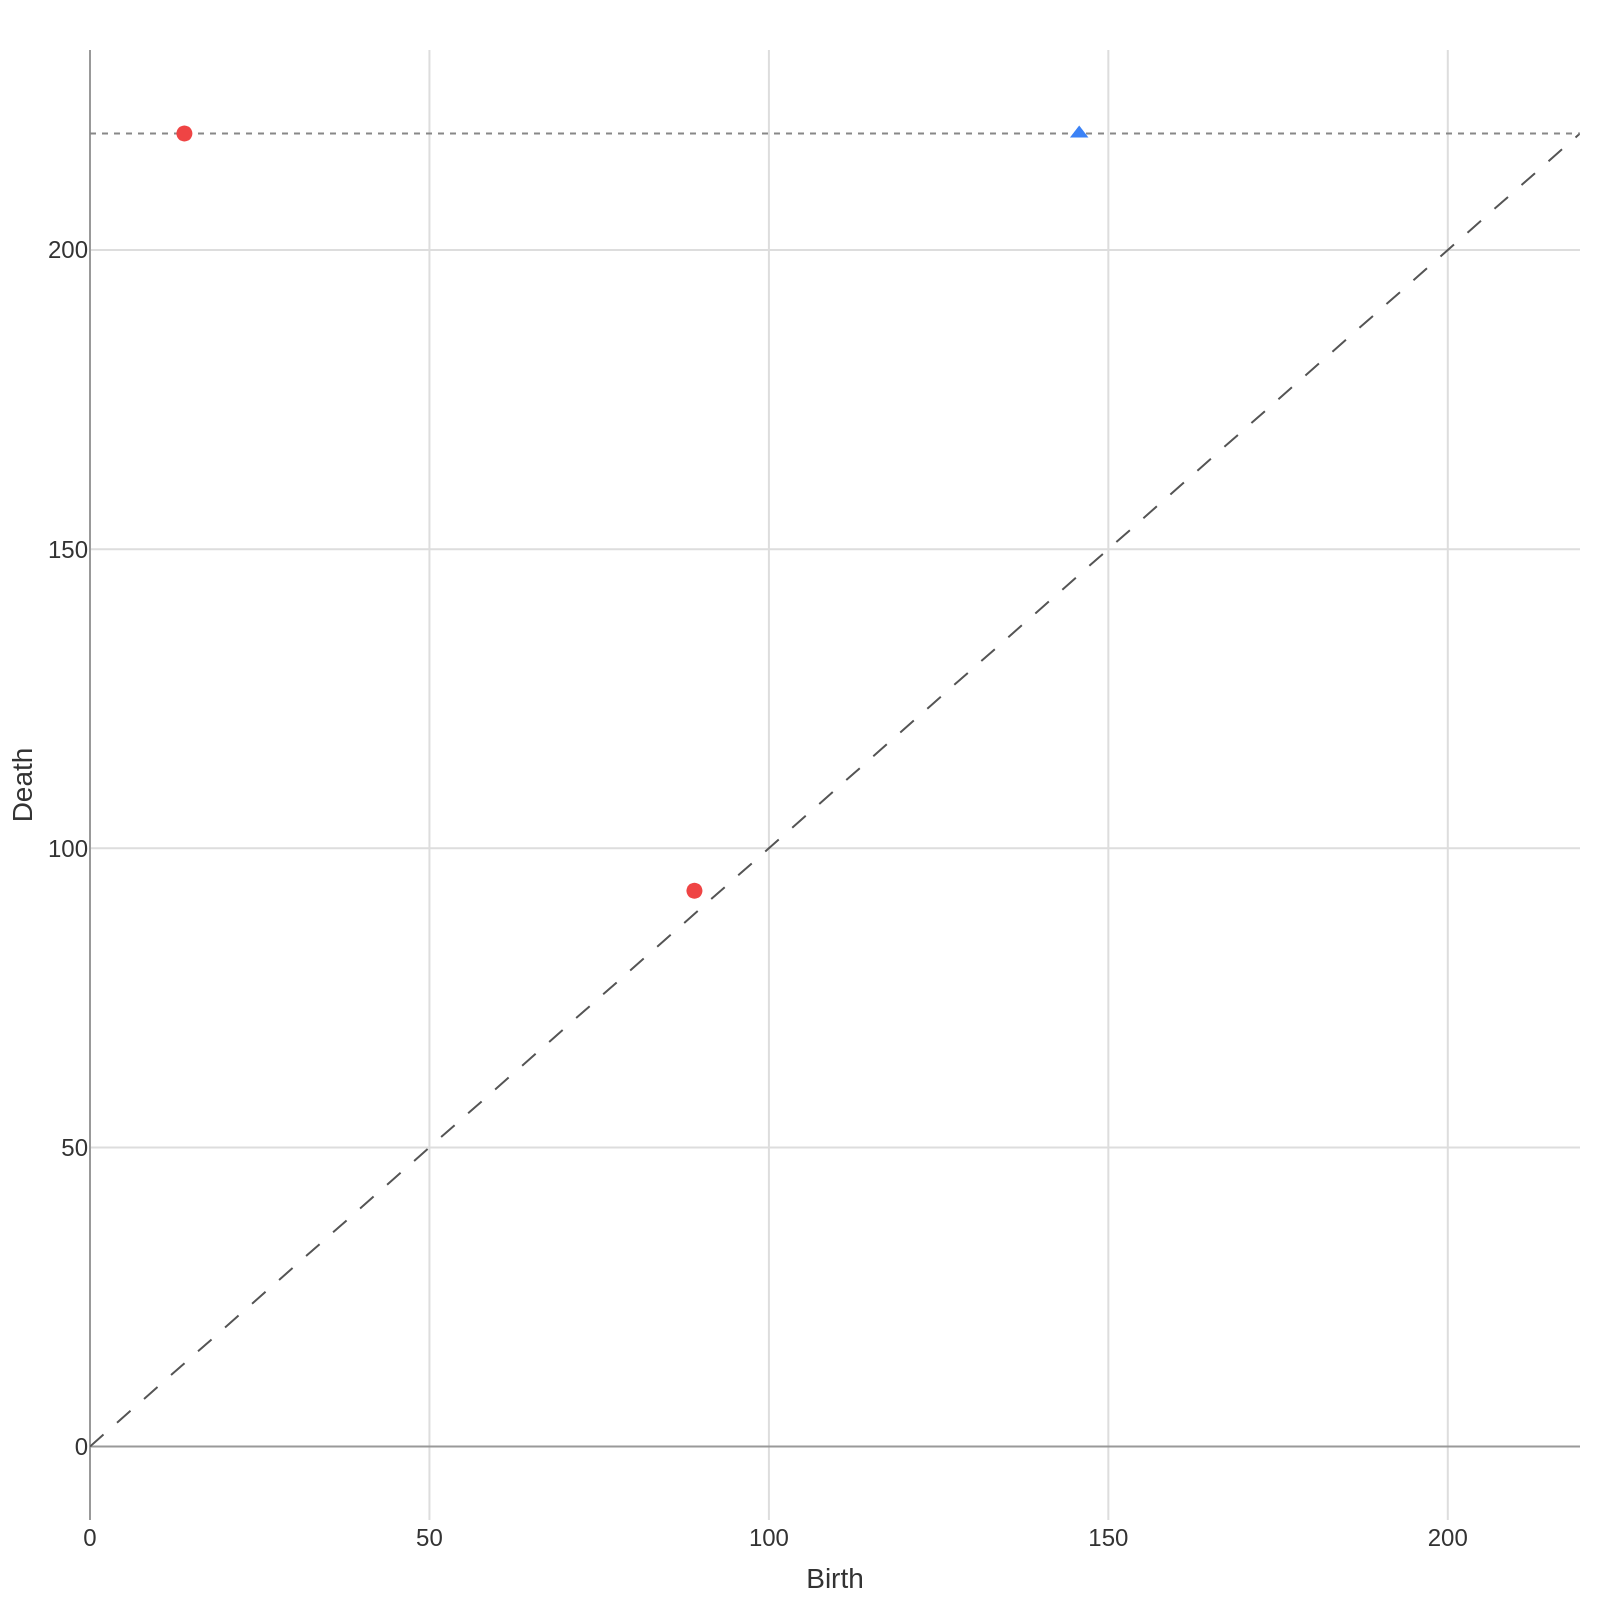
\includegraphics[width=0.27\textwidth]{persistence_diagram3.png}
        \caption{As the center crosses back through the focal set, the vineyard reappears.}
    \end{figure}
\end{frame}

\begin{frame}{Varying the Loop Radius}
    How does the vineyard change as the observation loop grows?
    \begin{figure}
        \centering
        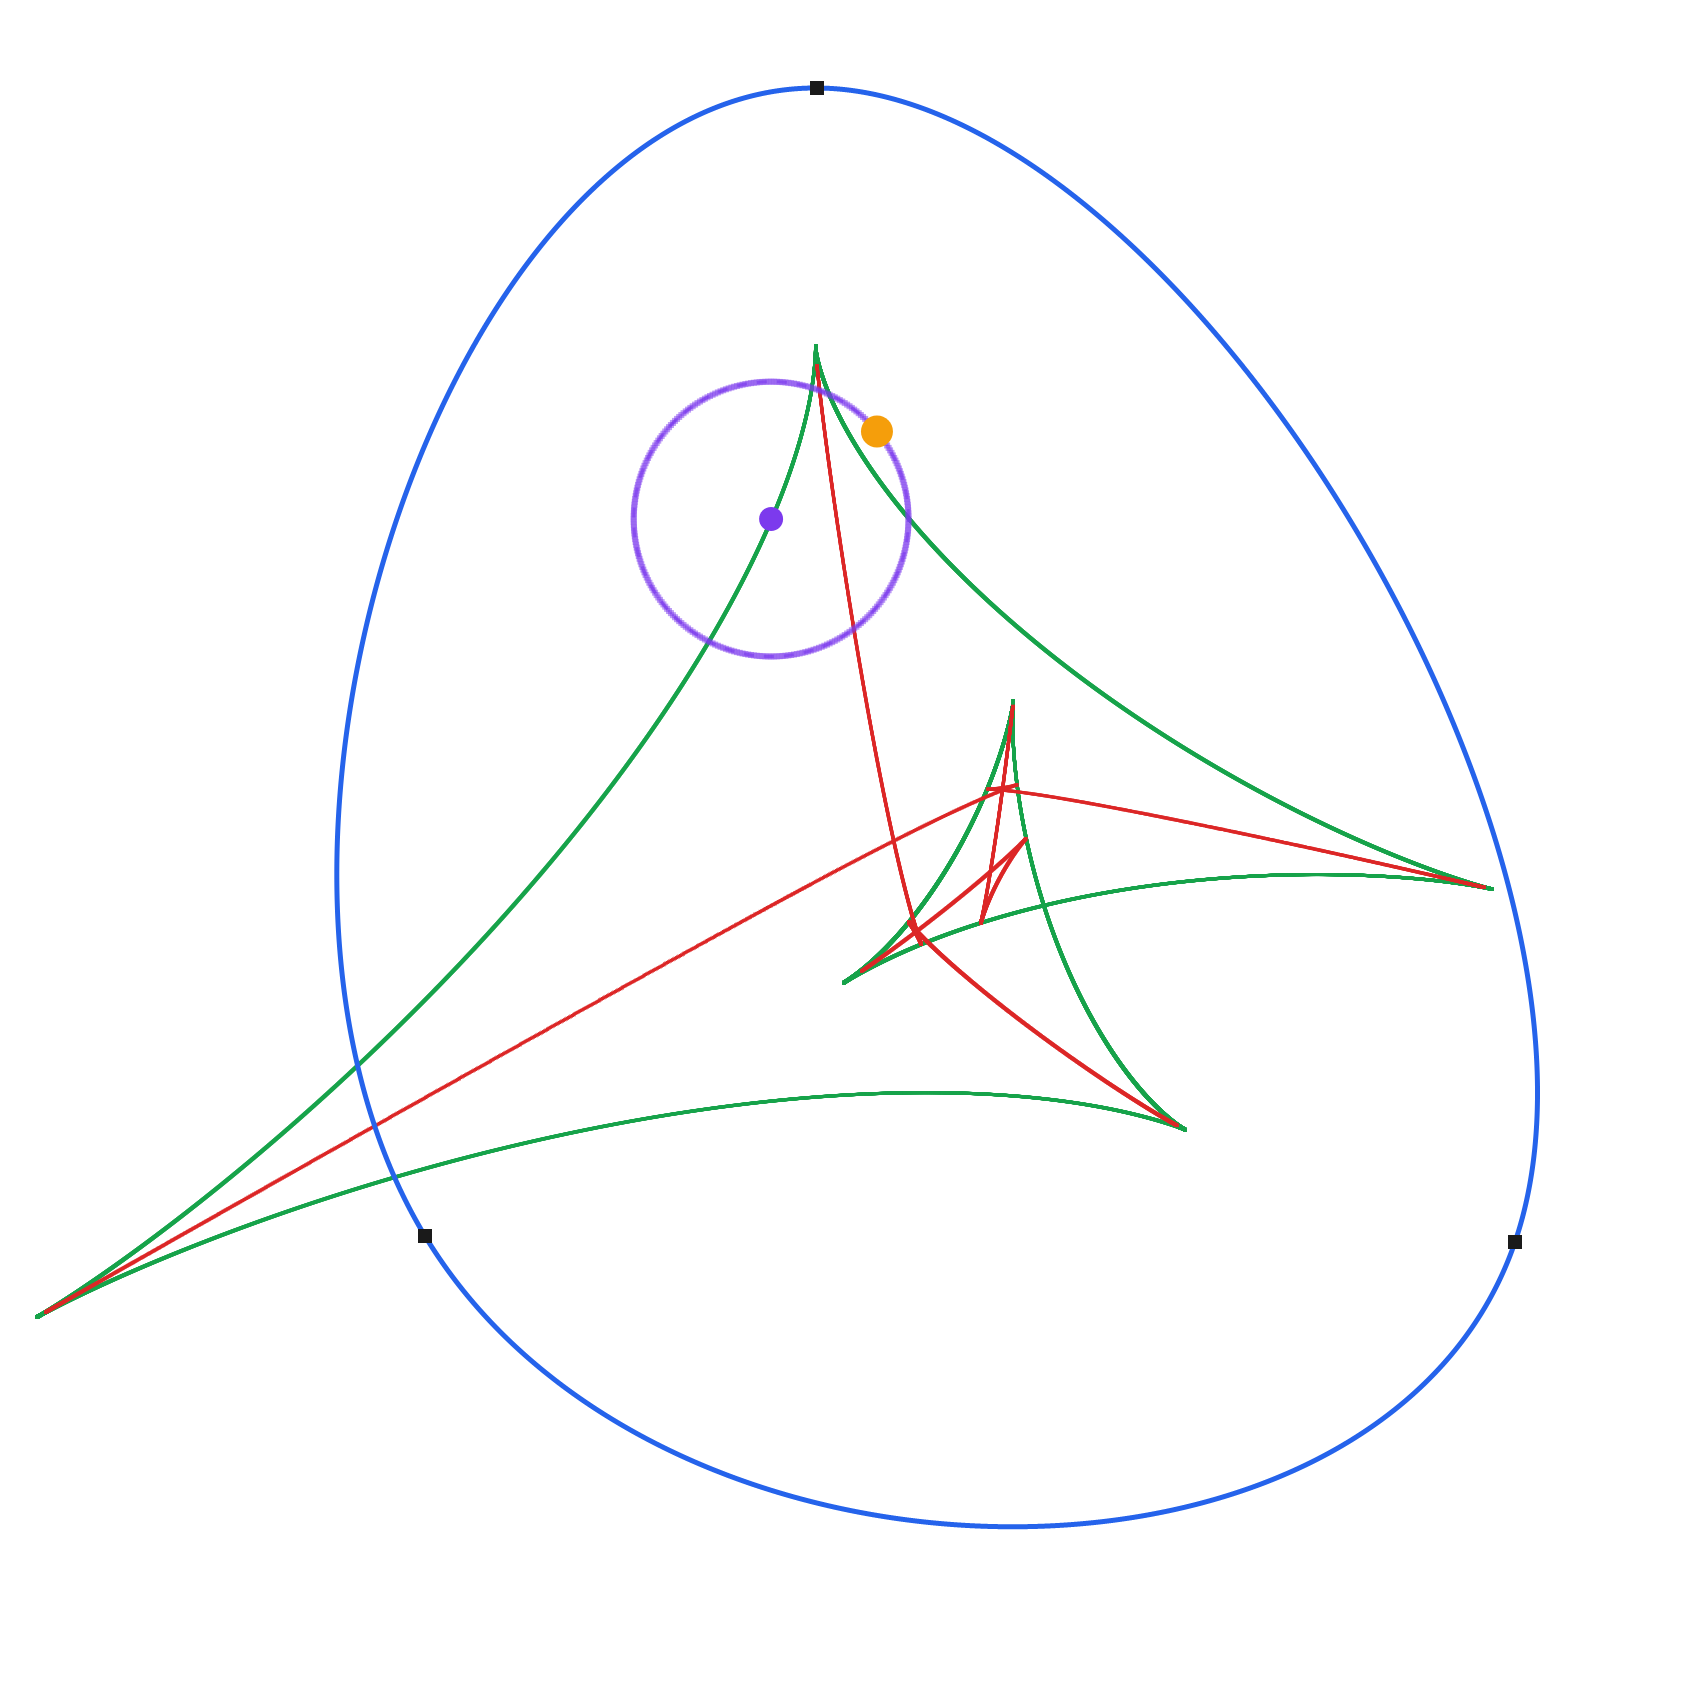
\includegraphics[width=0.42\linewidth]{canvas_r1.png}
        \hfill
        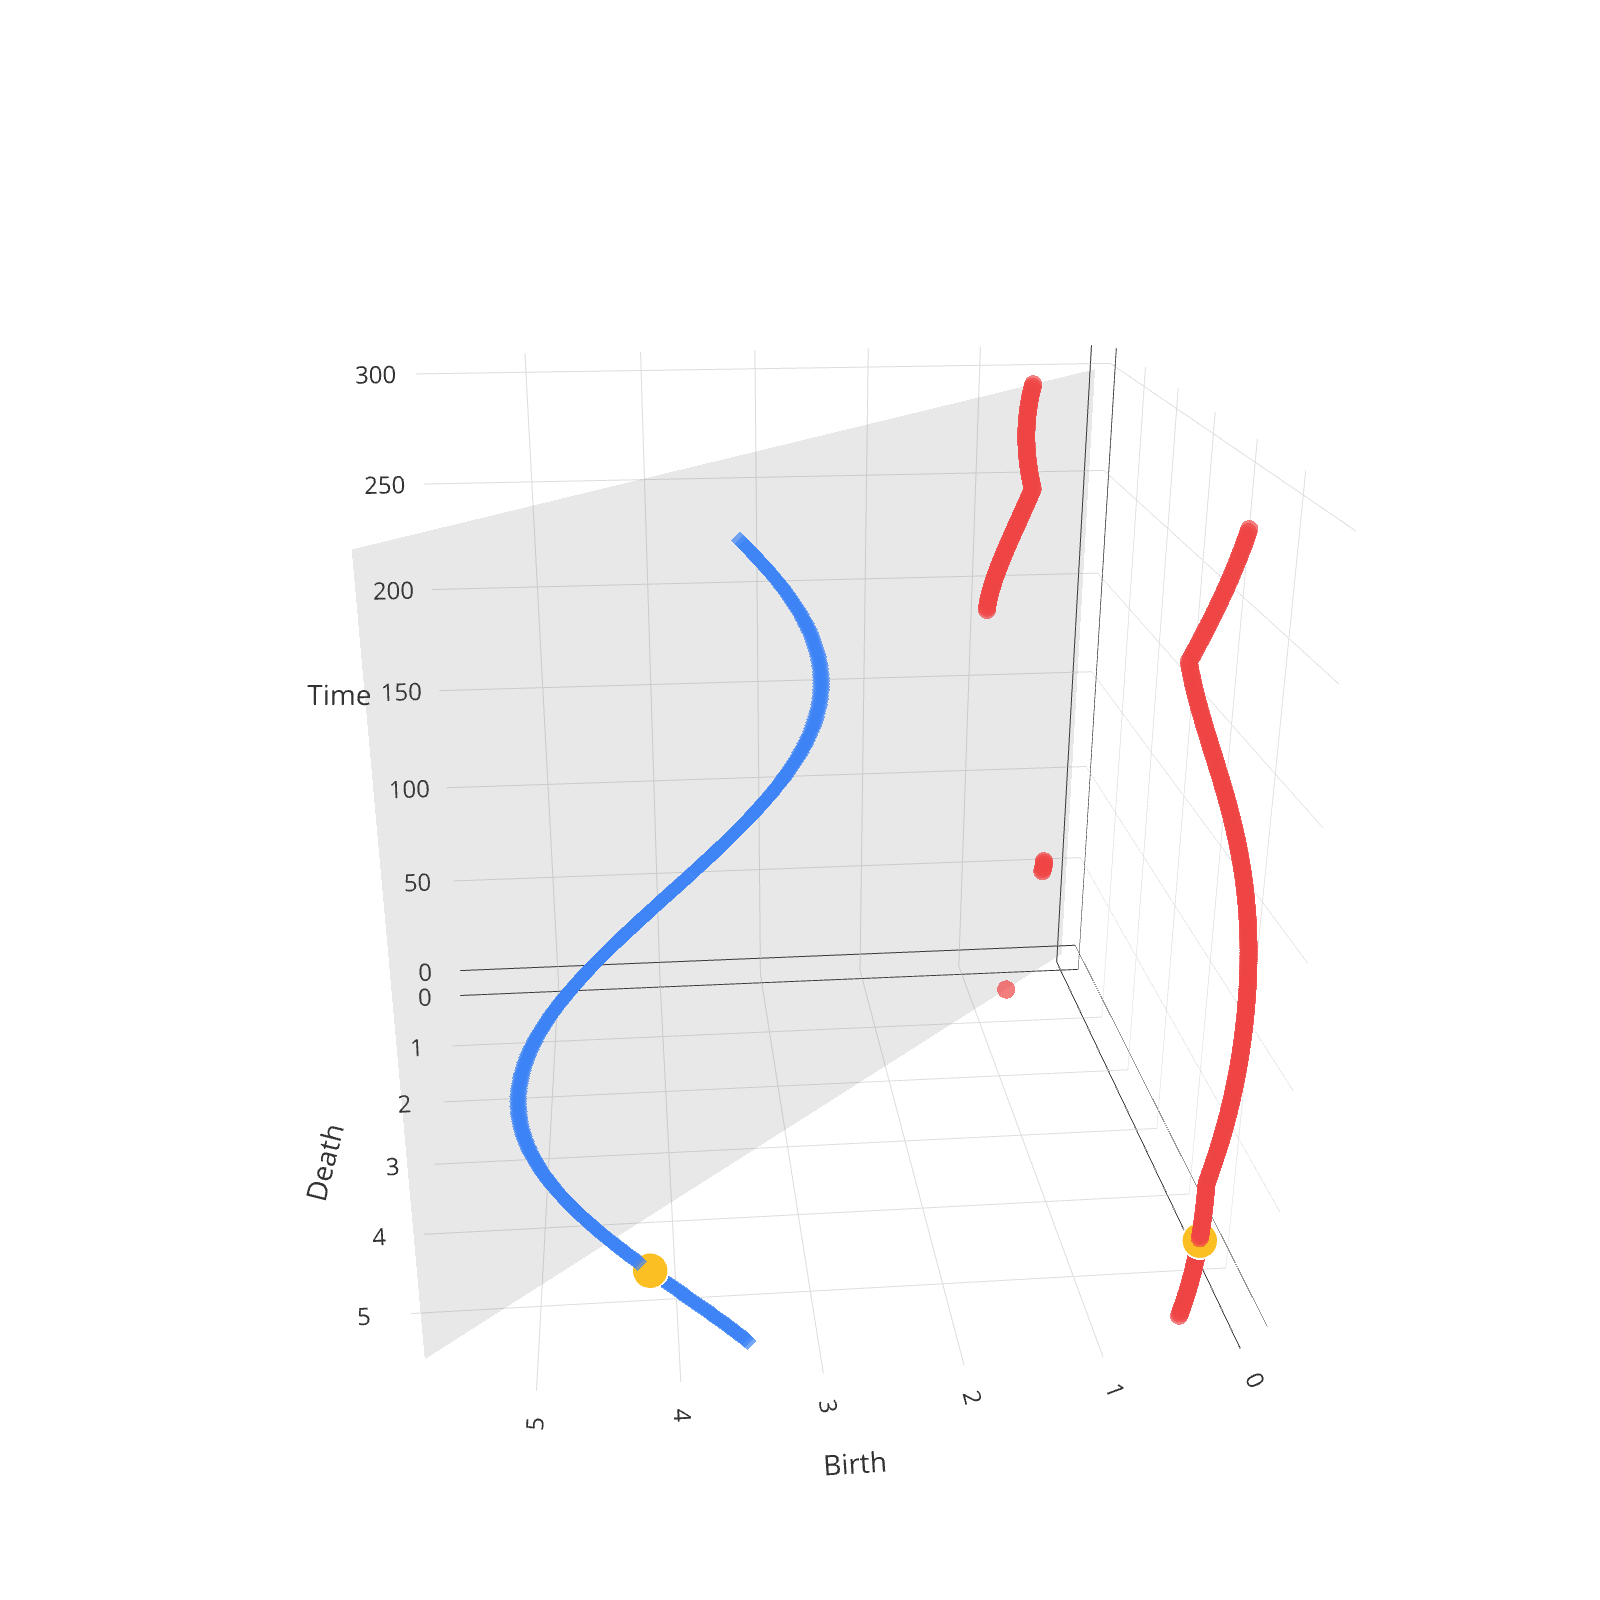
\includegraphics[width=0.42\linewidth]{vin_r1.png}

        \vspace{0.3em}

        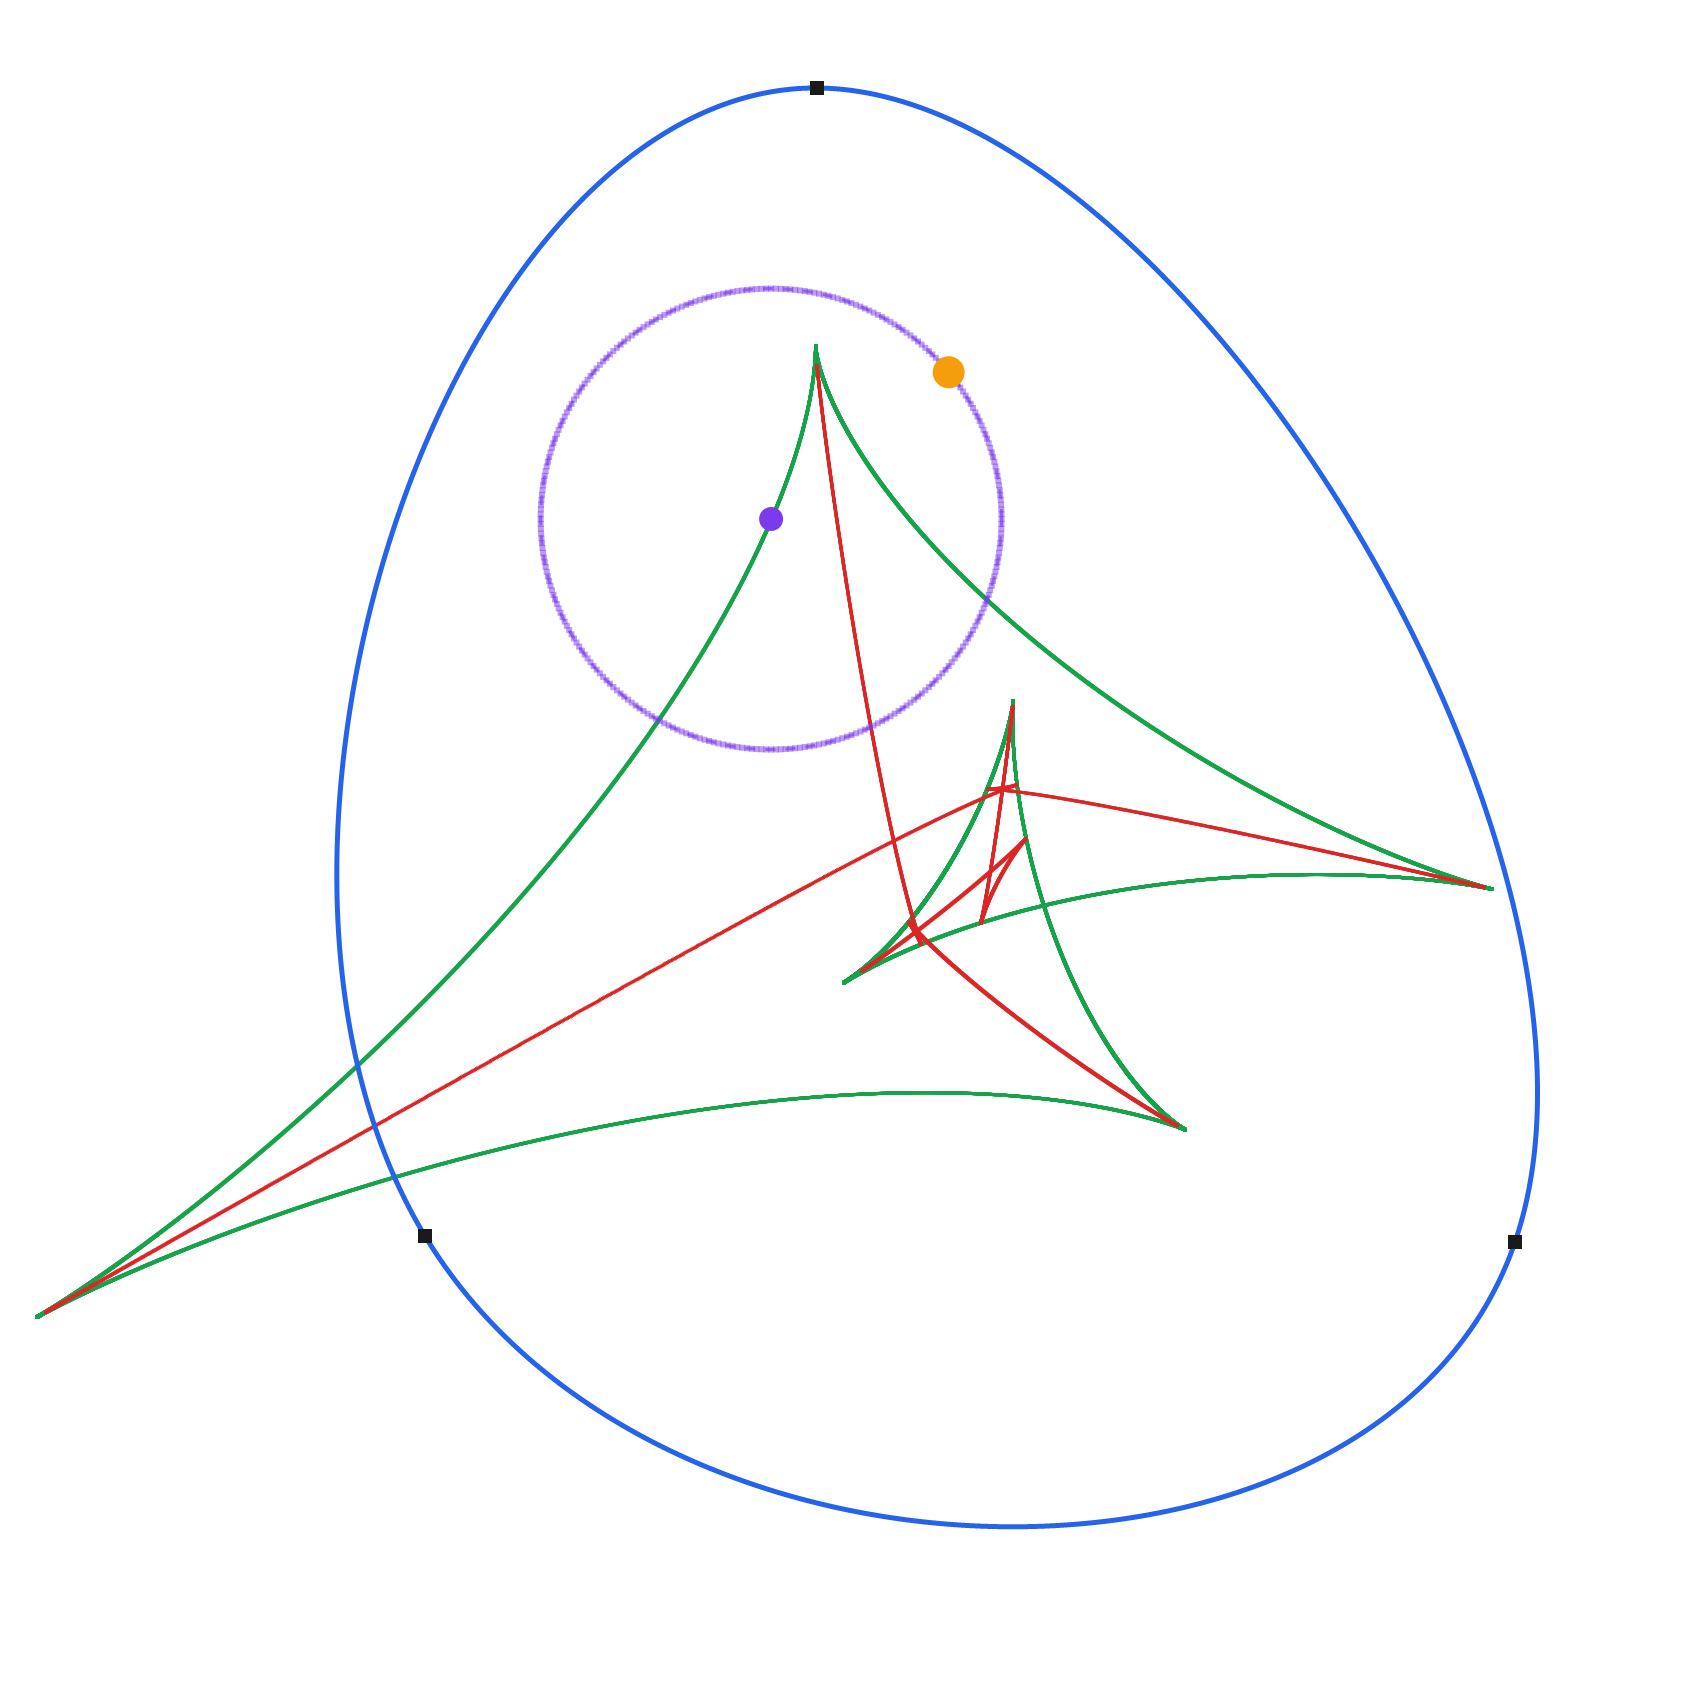
\includegraphics[width=0.42\linewidth]{canvas_r2.png}
        \hfill
        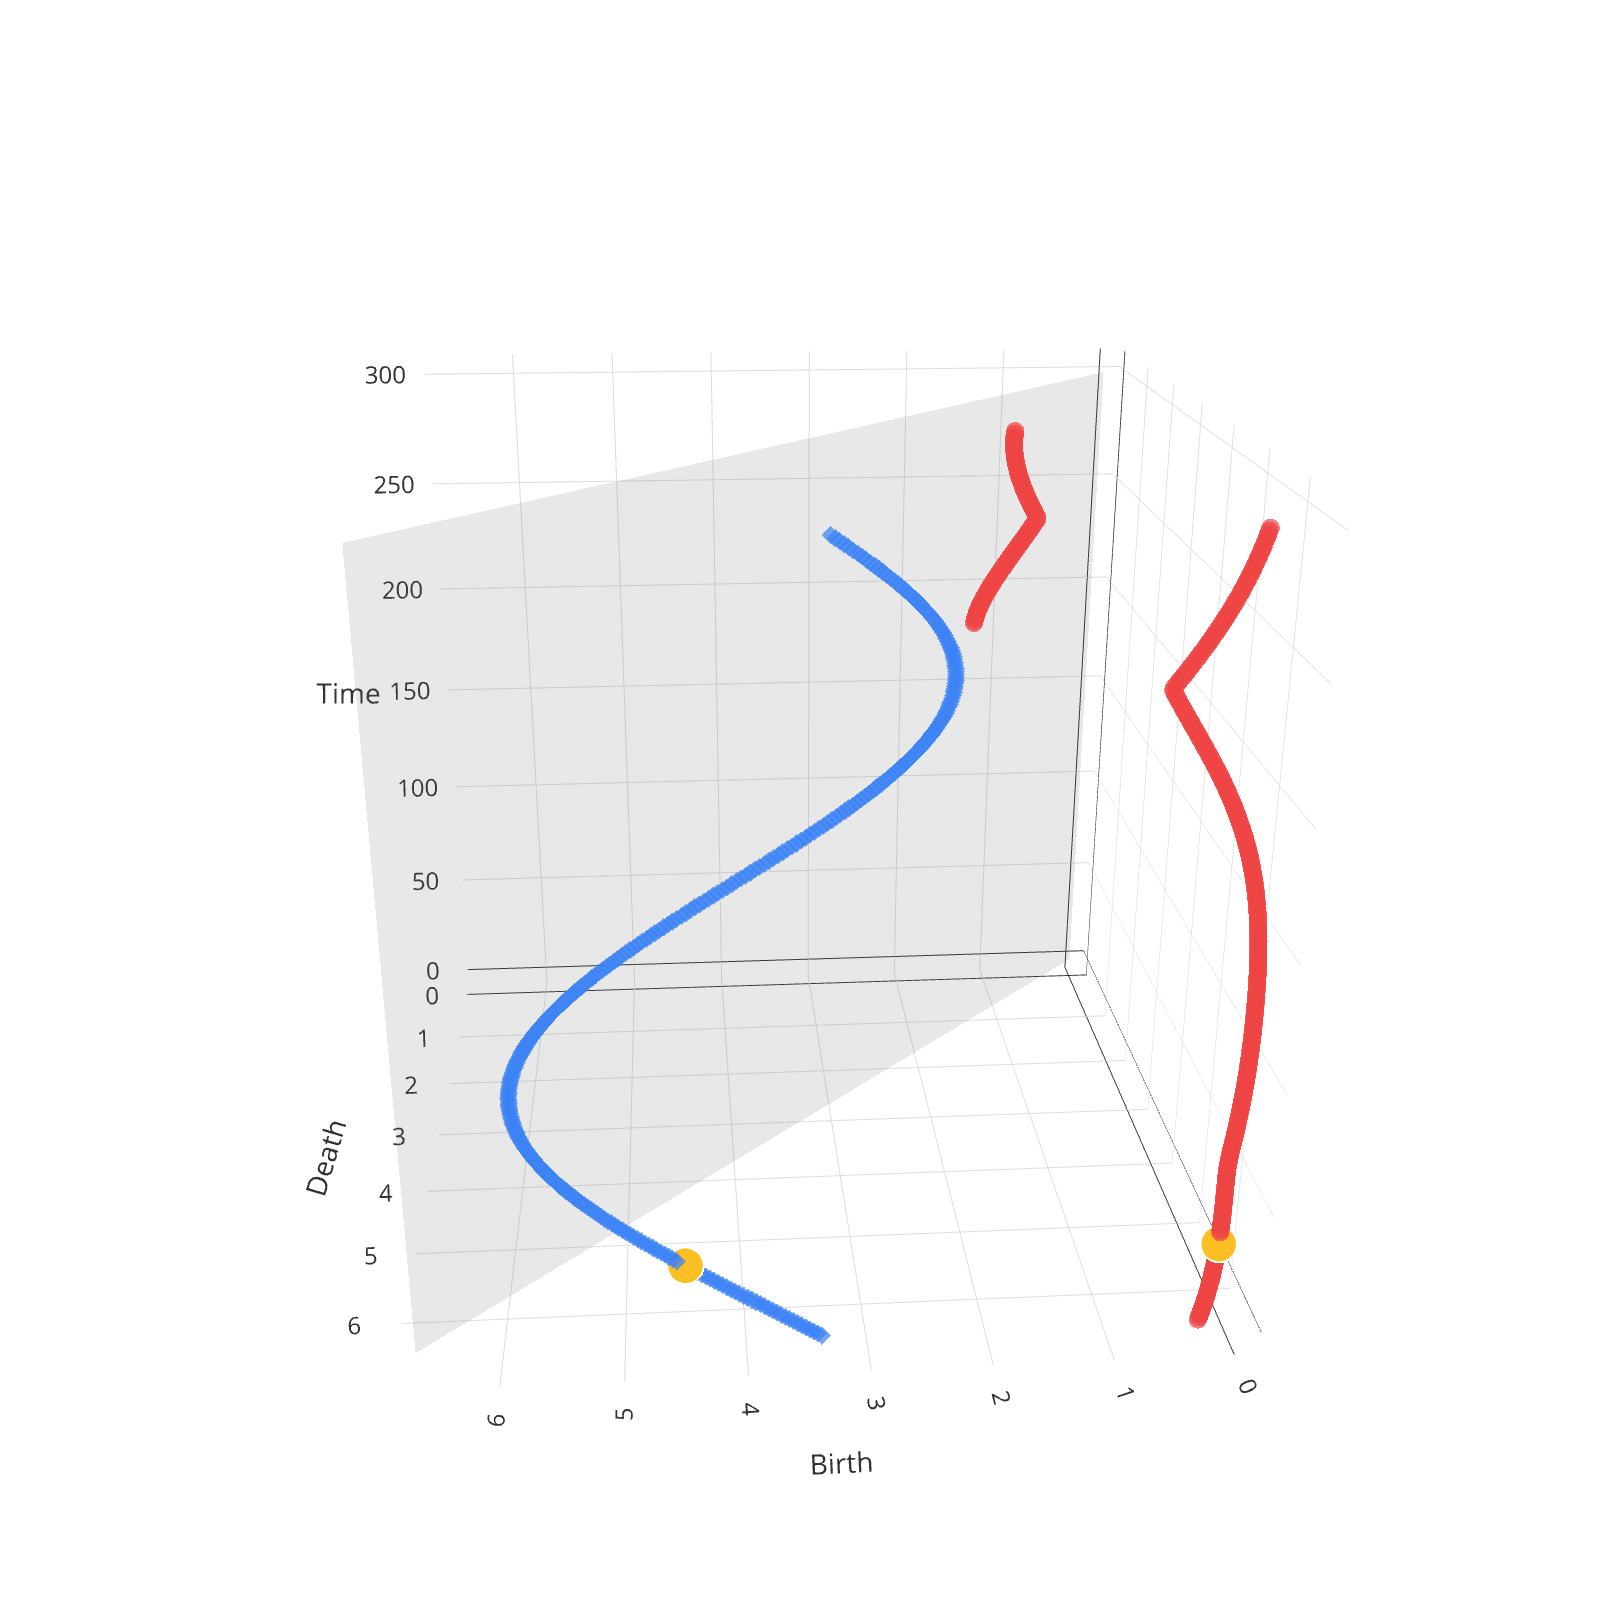
\includegraphics[width=0.42\linewidth]{vin_r2.png}

        \vspace{0.3em}

        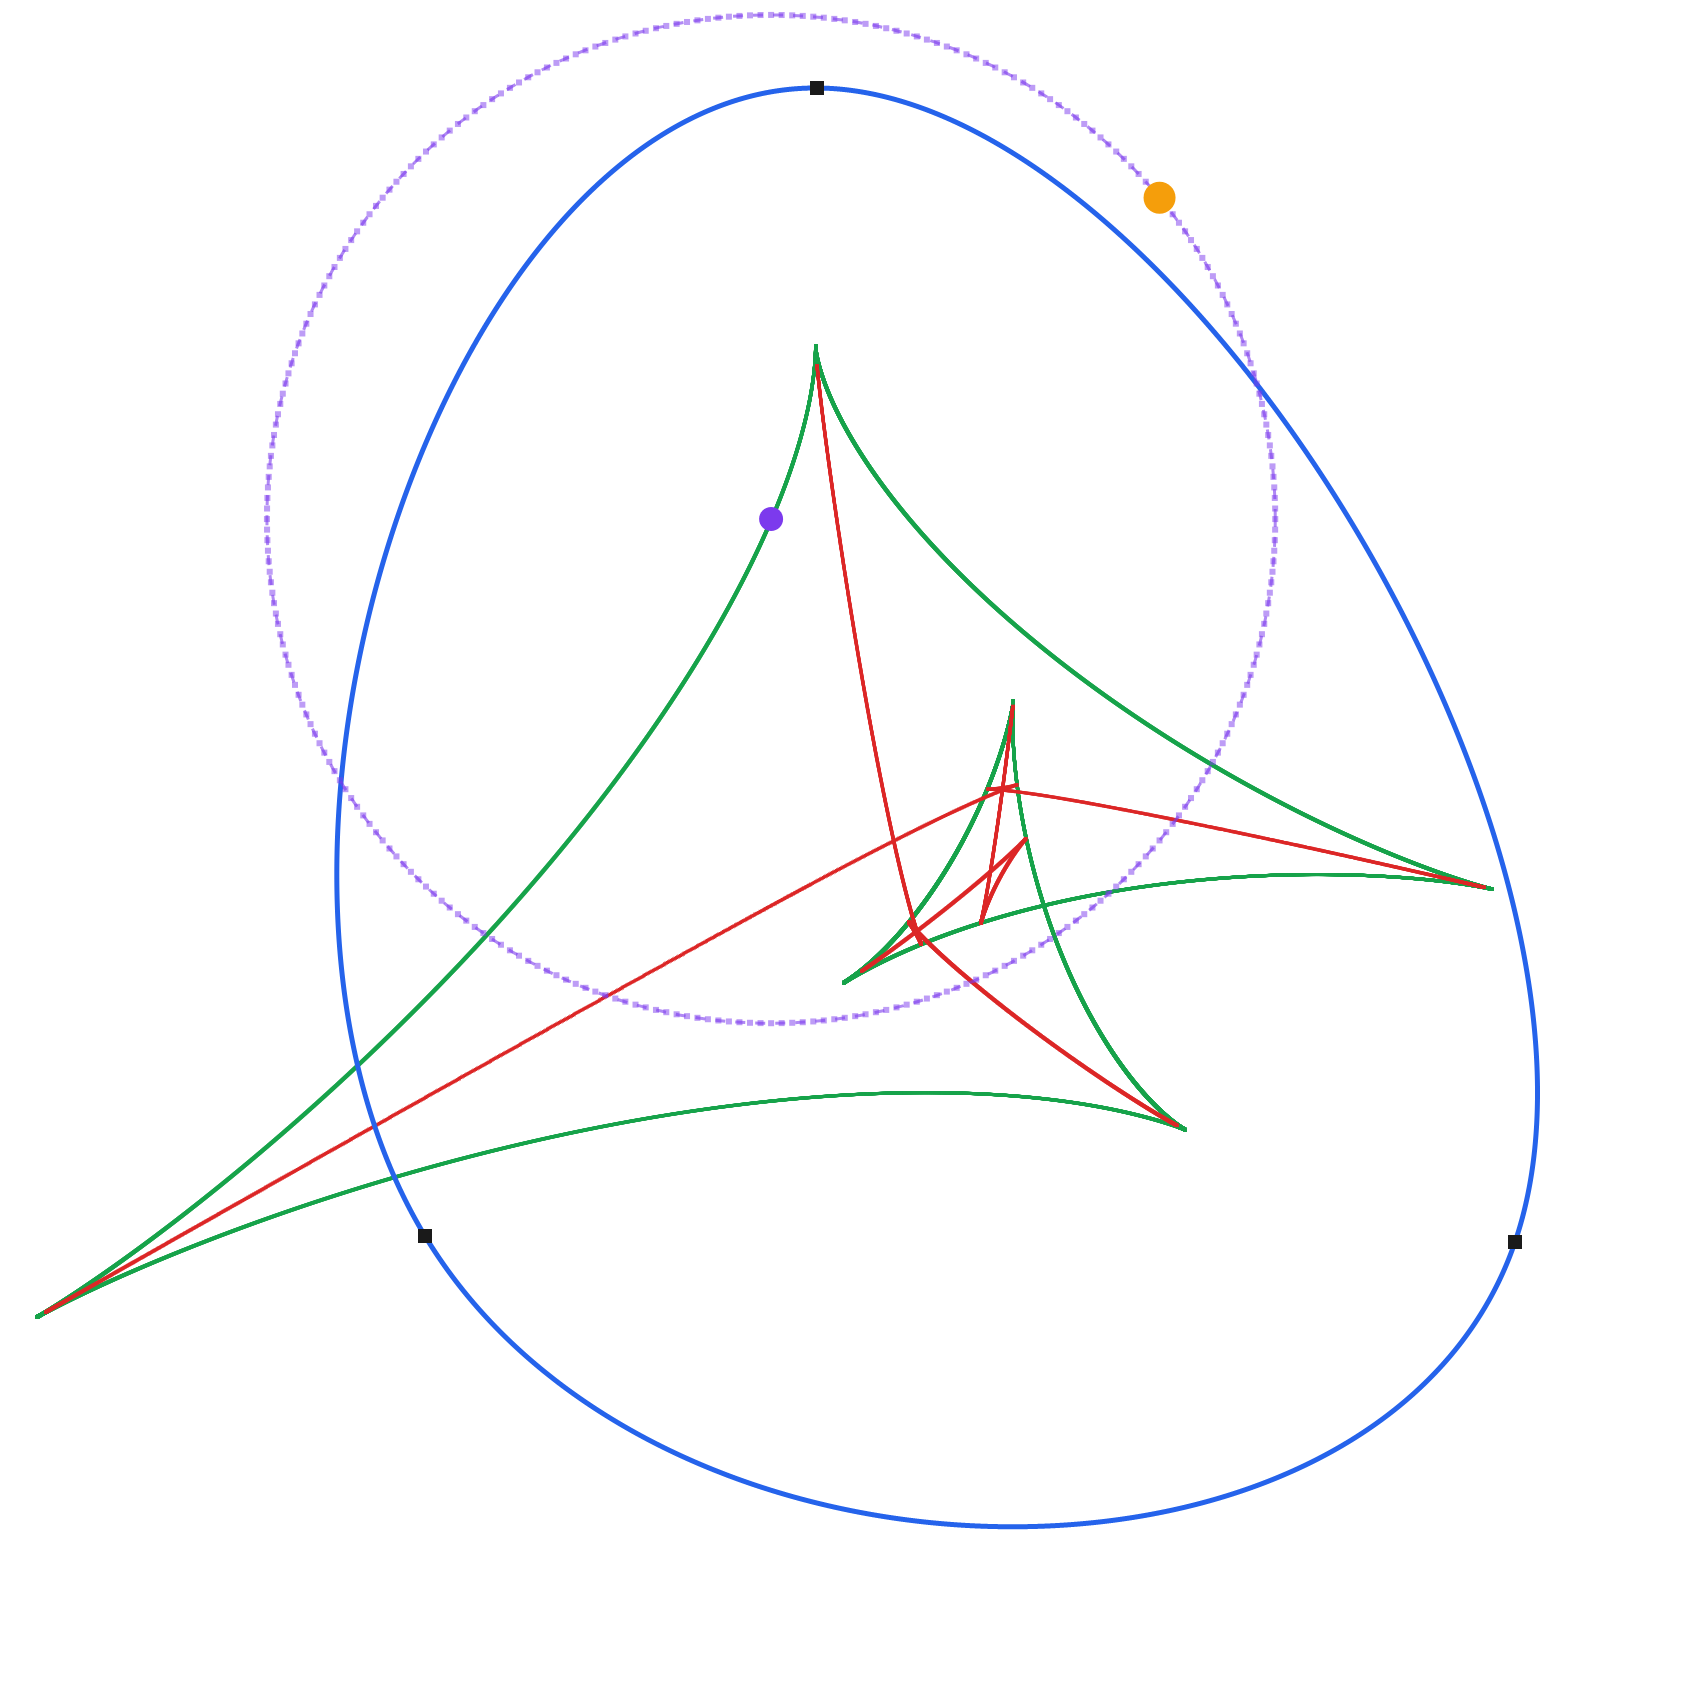
\includegraphics[width=0.42\linewidth]{canvas_r3.png}
        \hfill
        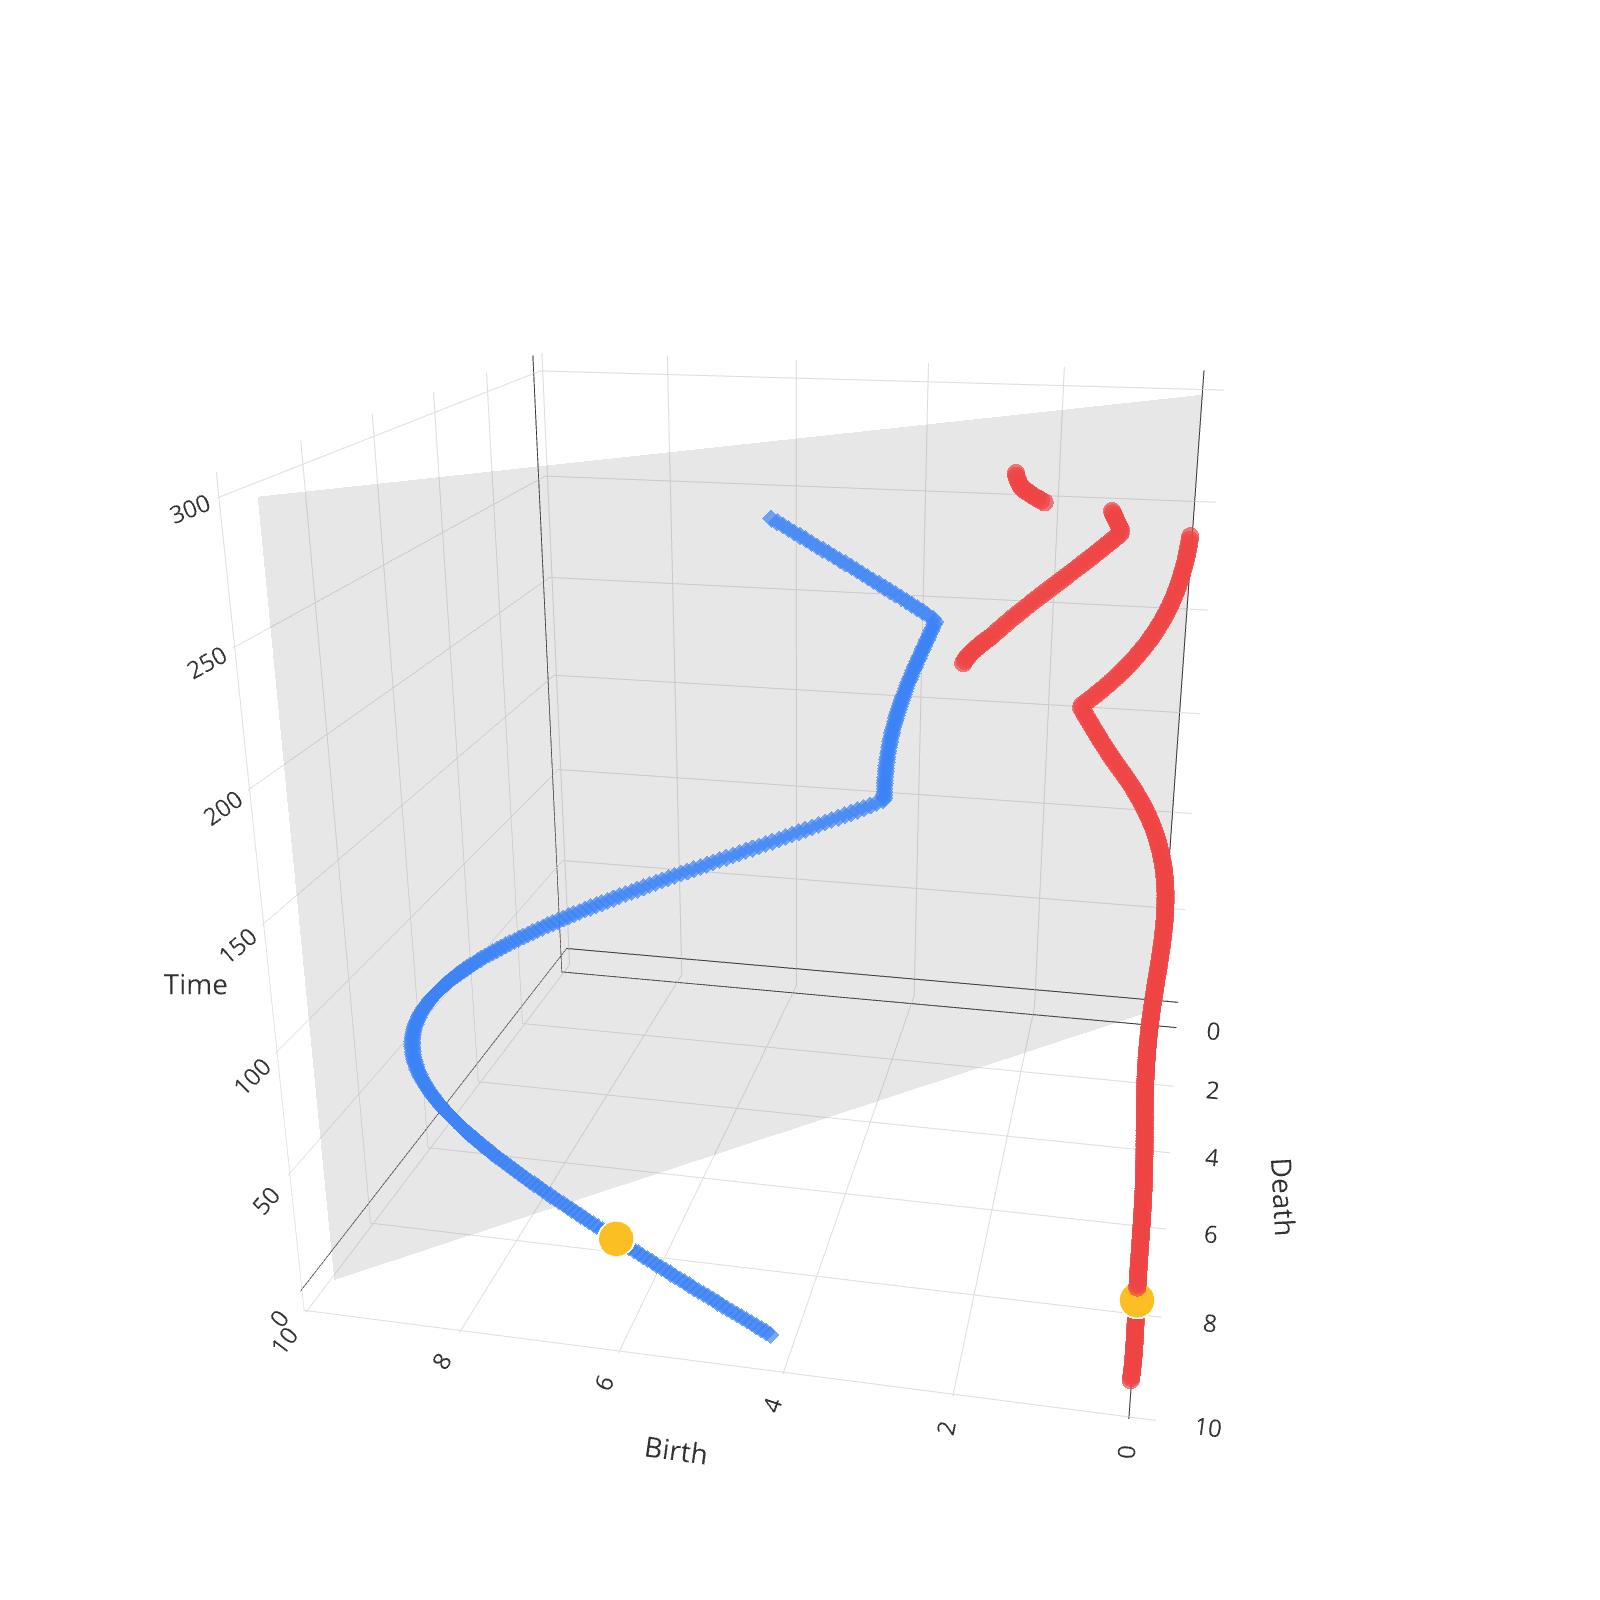
\includegraphics[width=0.42\linewidth]{vin_r3.png}
        \caption{Vines evolve as the loop encompasses different topological features.}
    \end{figure}
\end{frame}

\begin{frame}{Two Components and Spline Loops}
    \begin{columns}[T]
        \begin{column}{0.48\textwidth}
            \textbf{Two disjoint components} with extended persistence:
            \begin{figure}
                \centering
                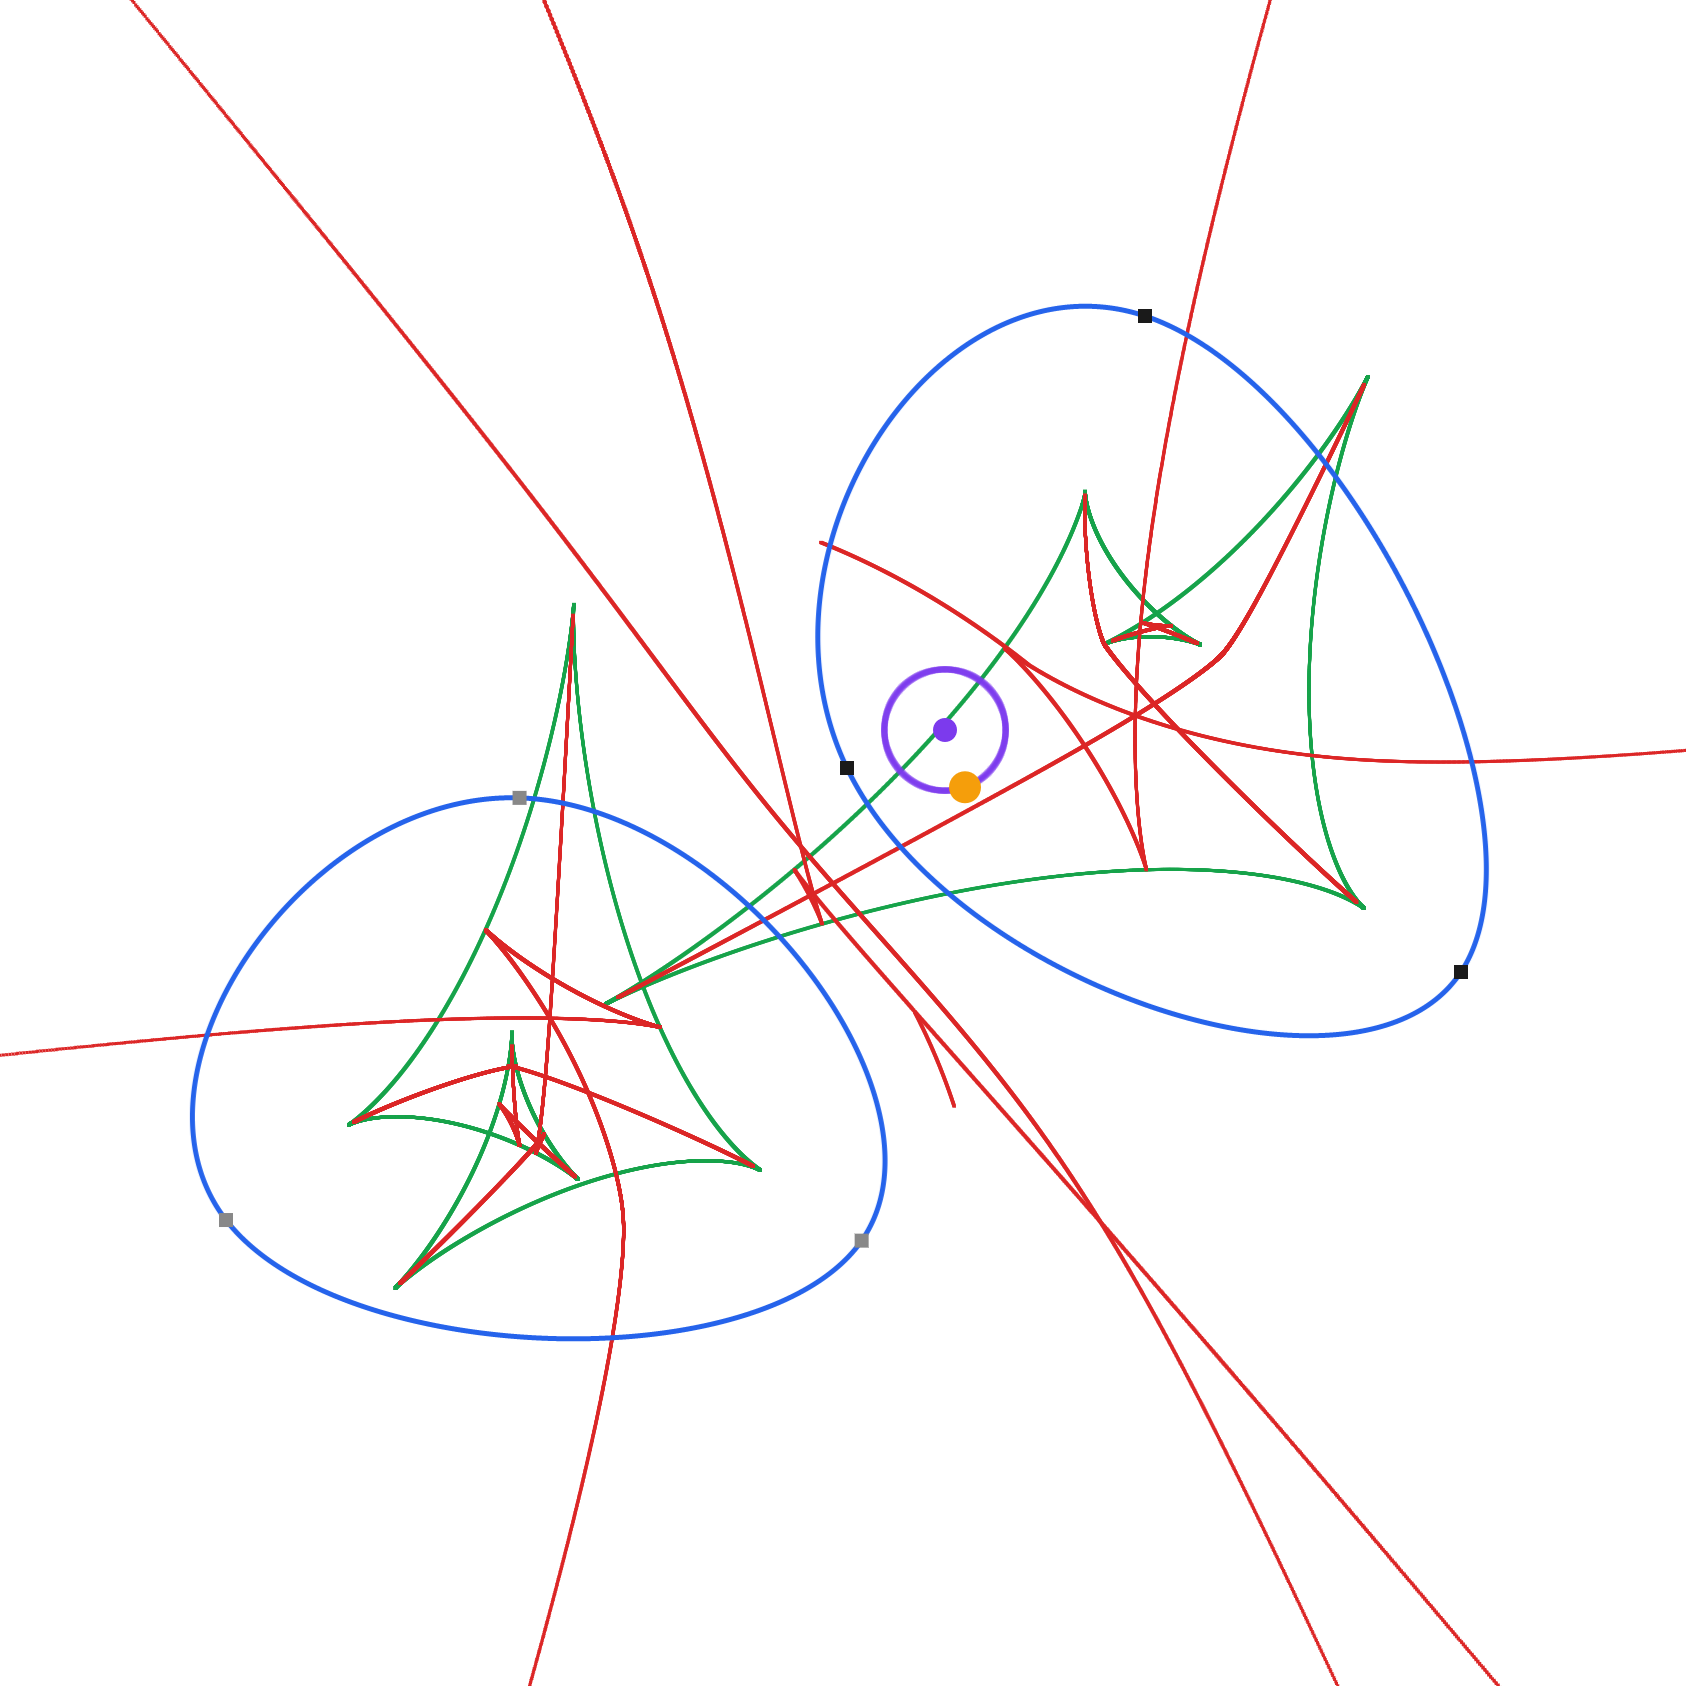
\includegraphics[width=\linewidth]{2_comp_vin.png}

                \vspace{0.2em}

                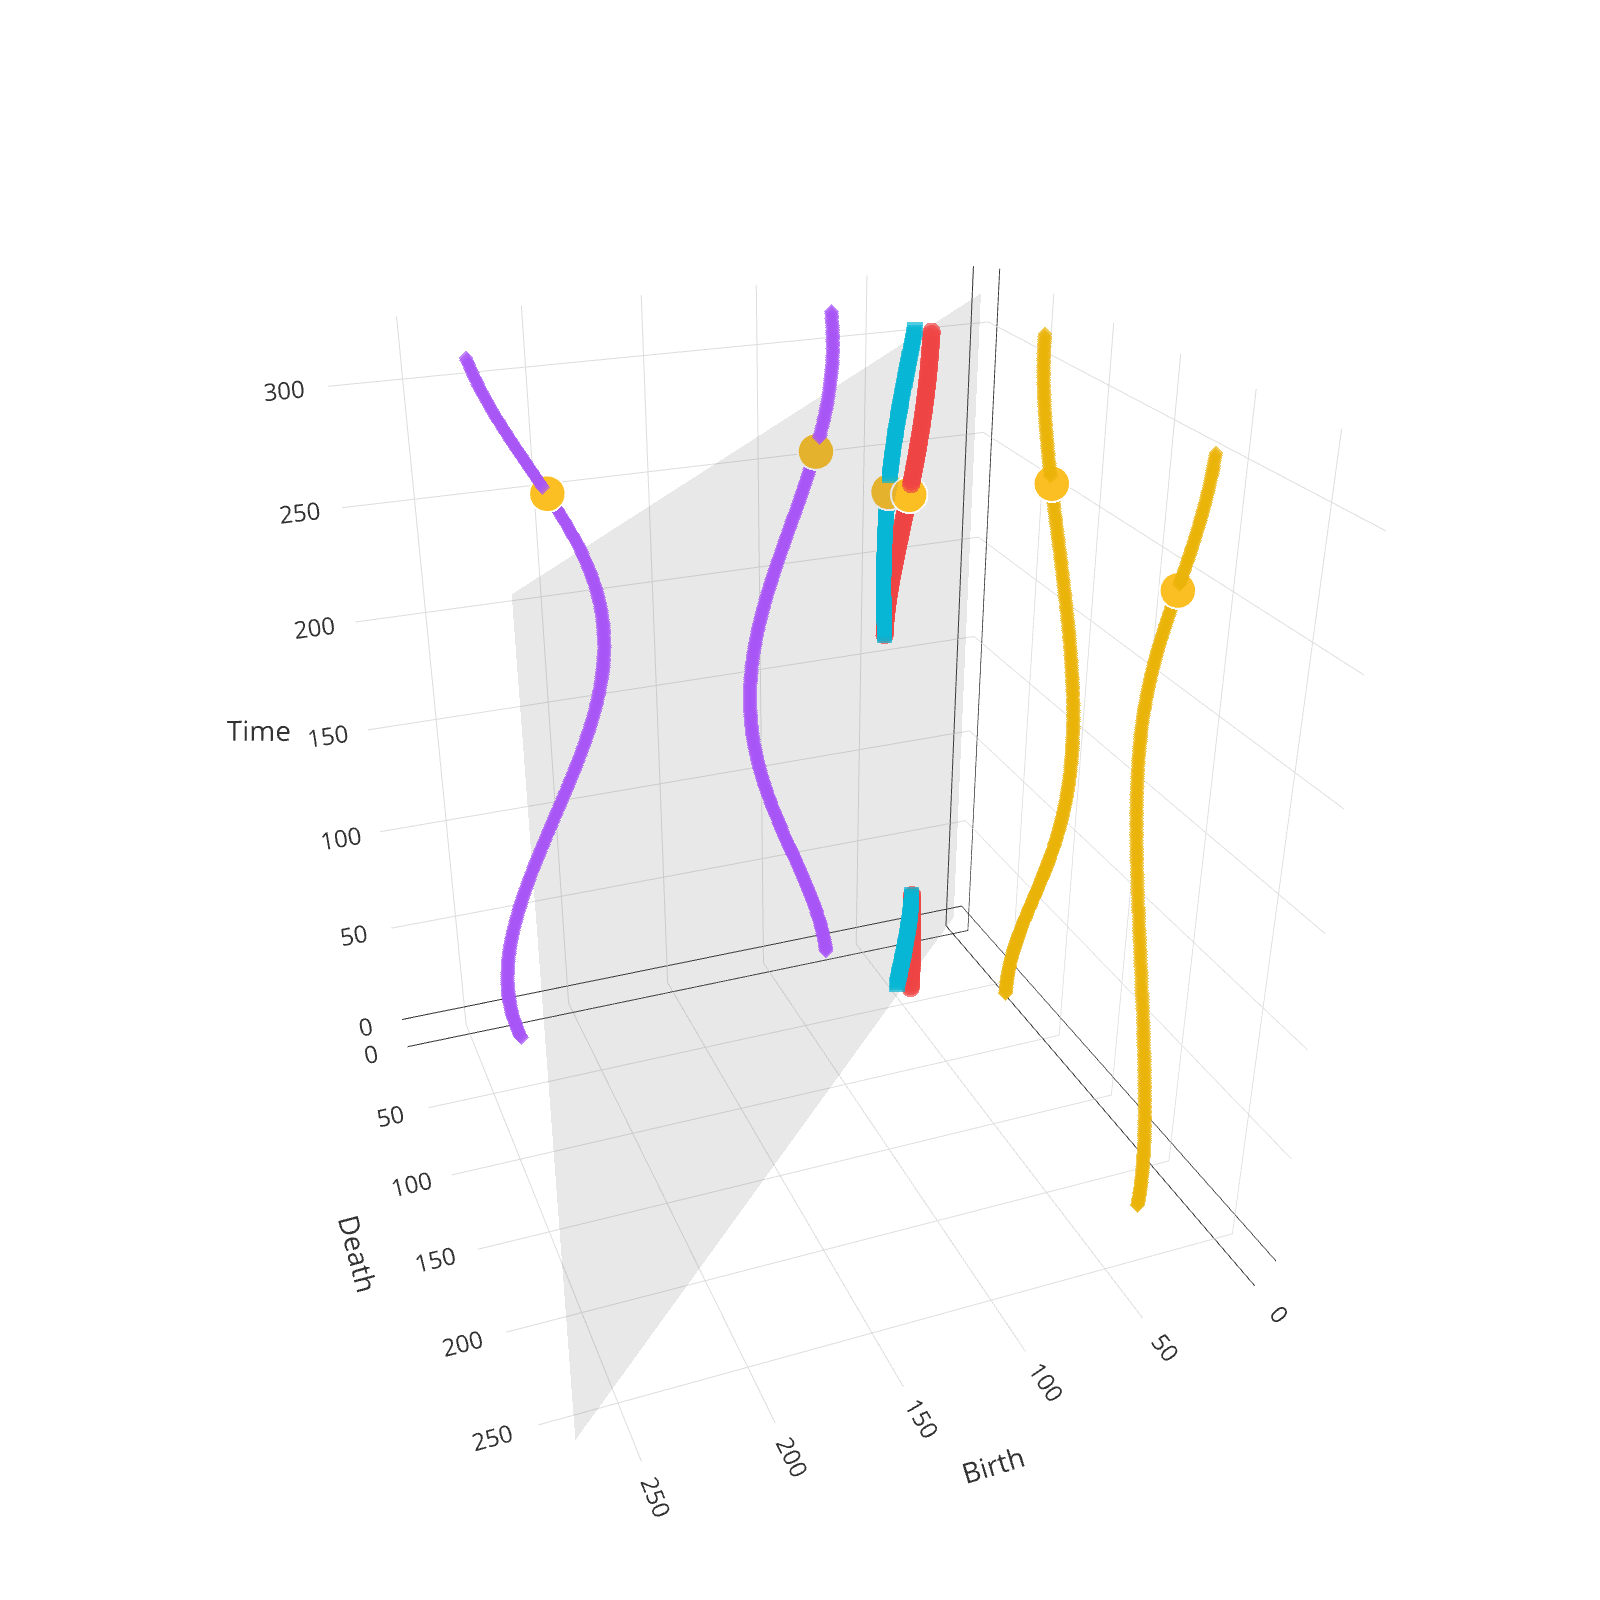
\includegraphics[width=\linewidth]{vin_2_comp.png}
            \end{figure}
        \end{column}
        \begin{column}{0.48\textwidth}
            \textbf{Hand-drawn spline loop} as observation path:
            \begin{figure}
                \centering
                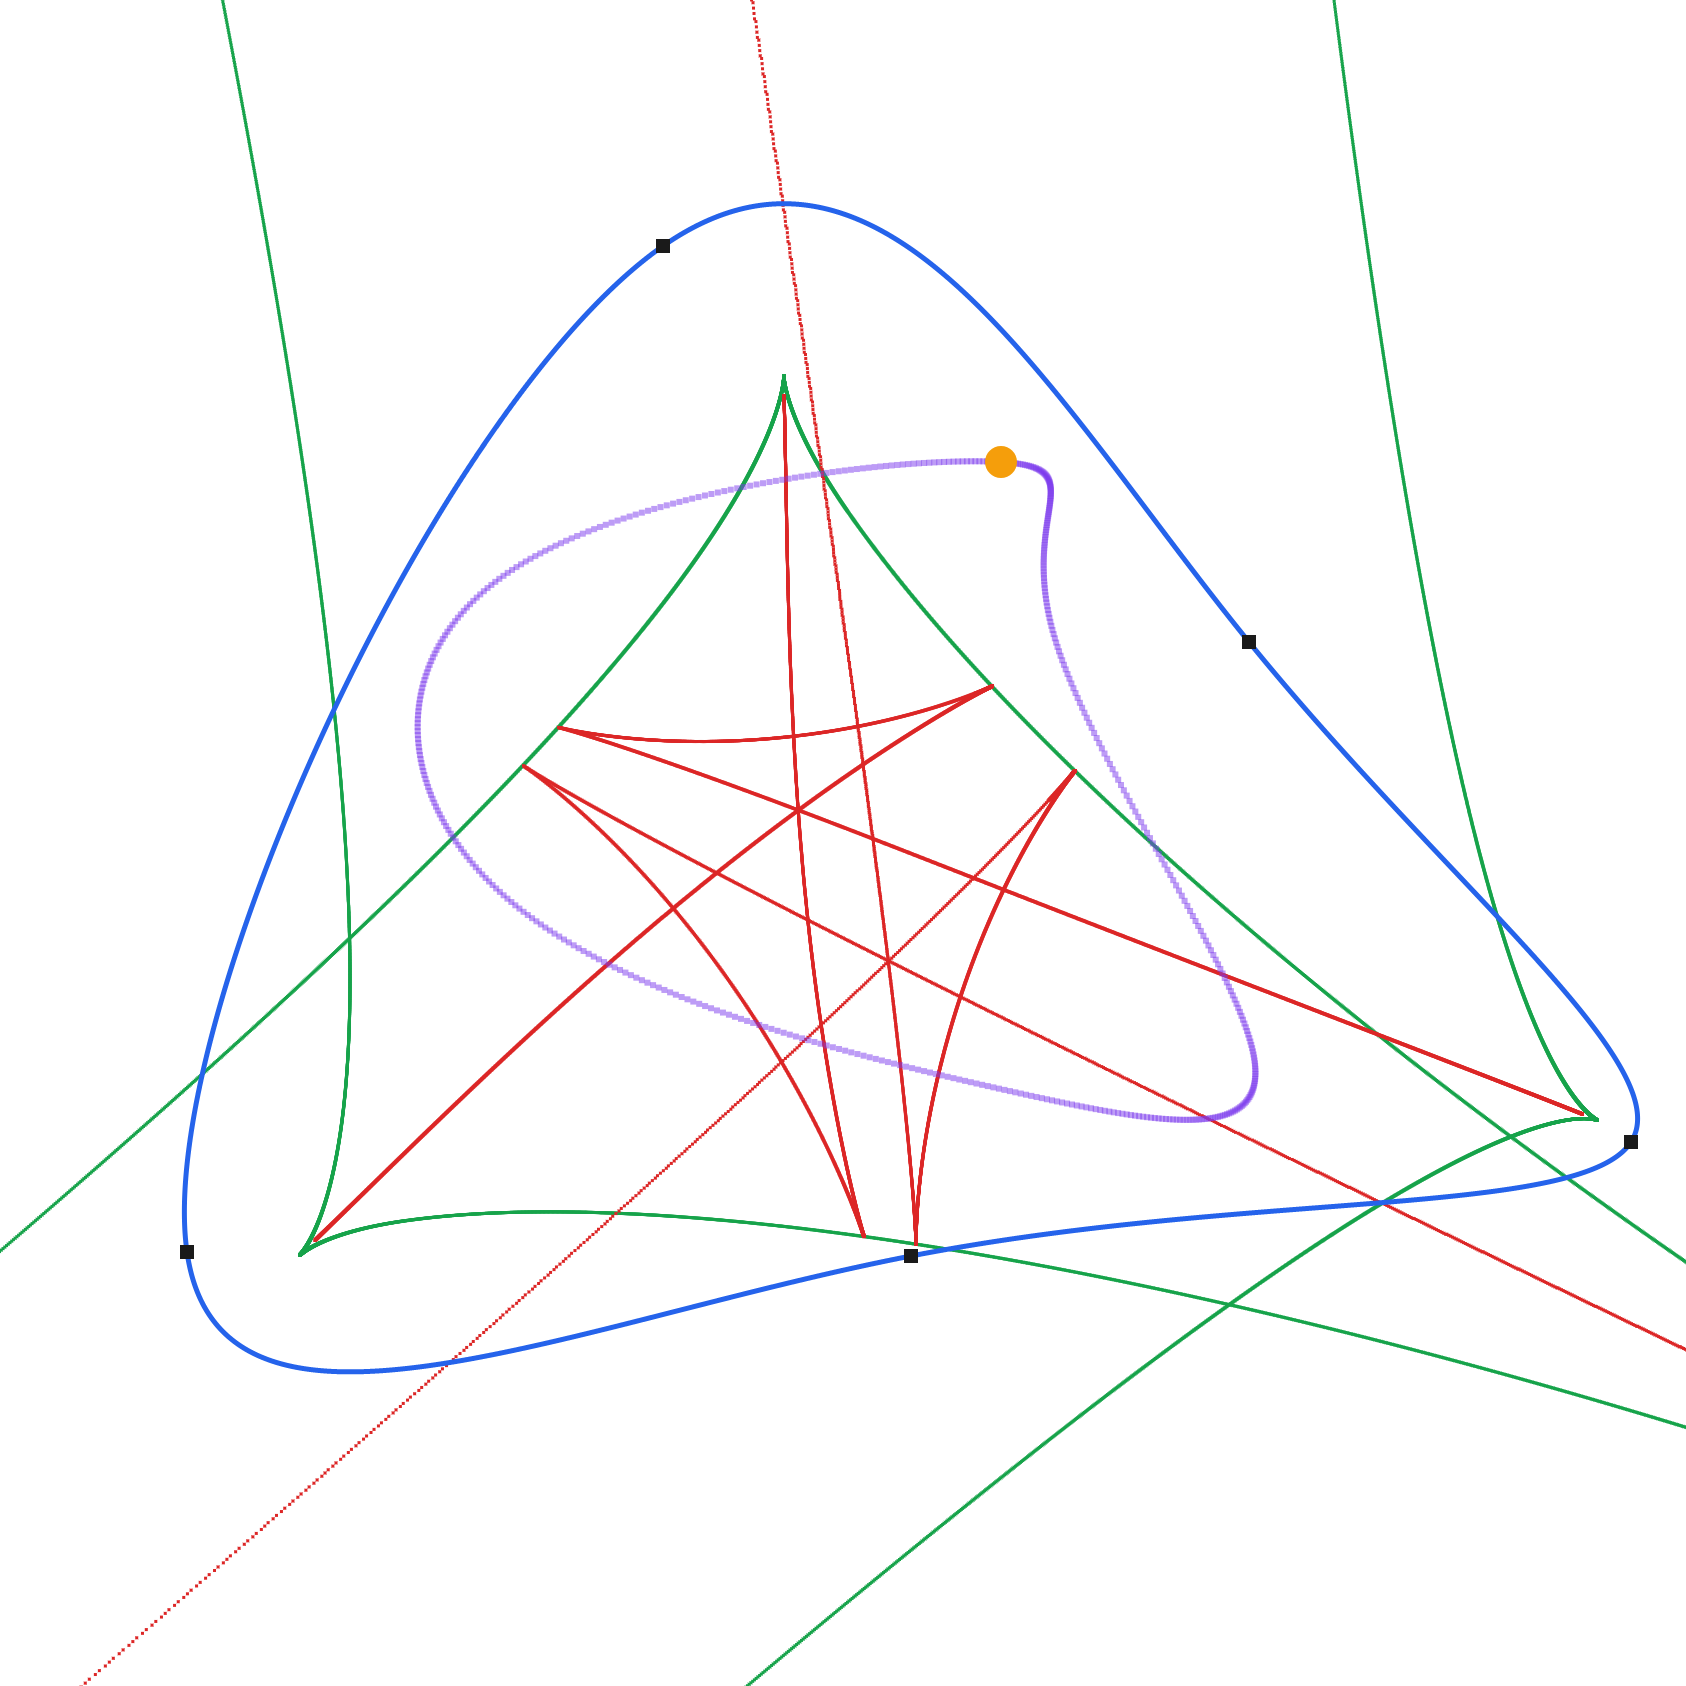
\includegraphics[width=\linewidth]{canvas_spline.png}

                \vspace{0.2em}

                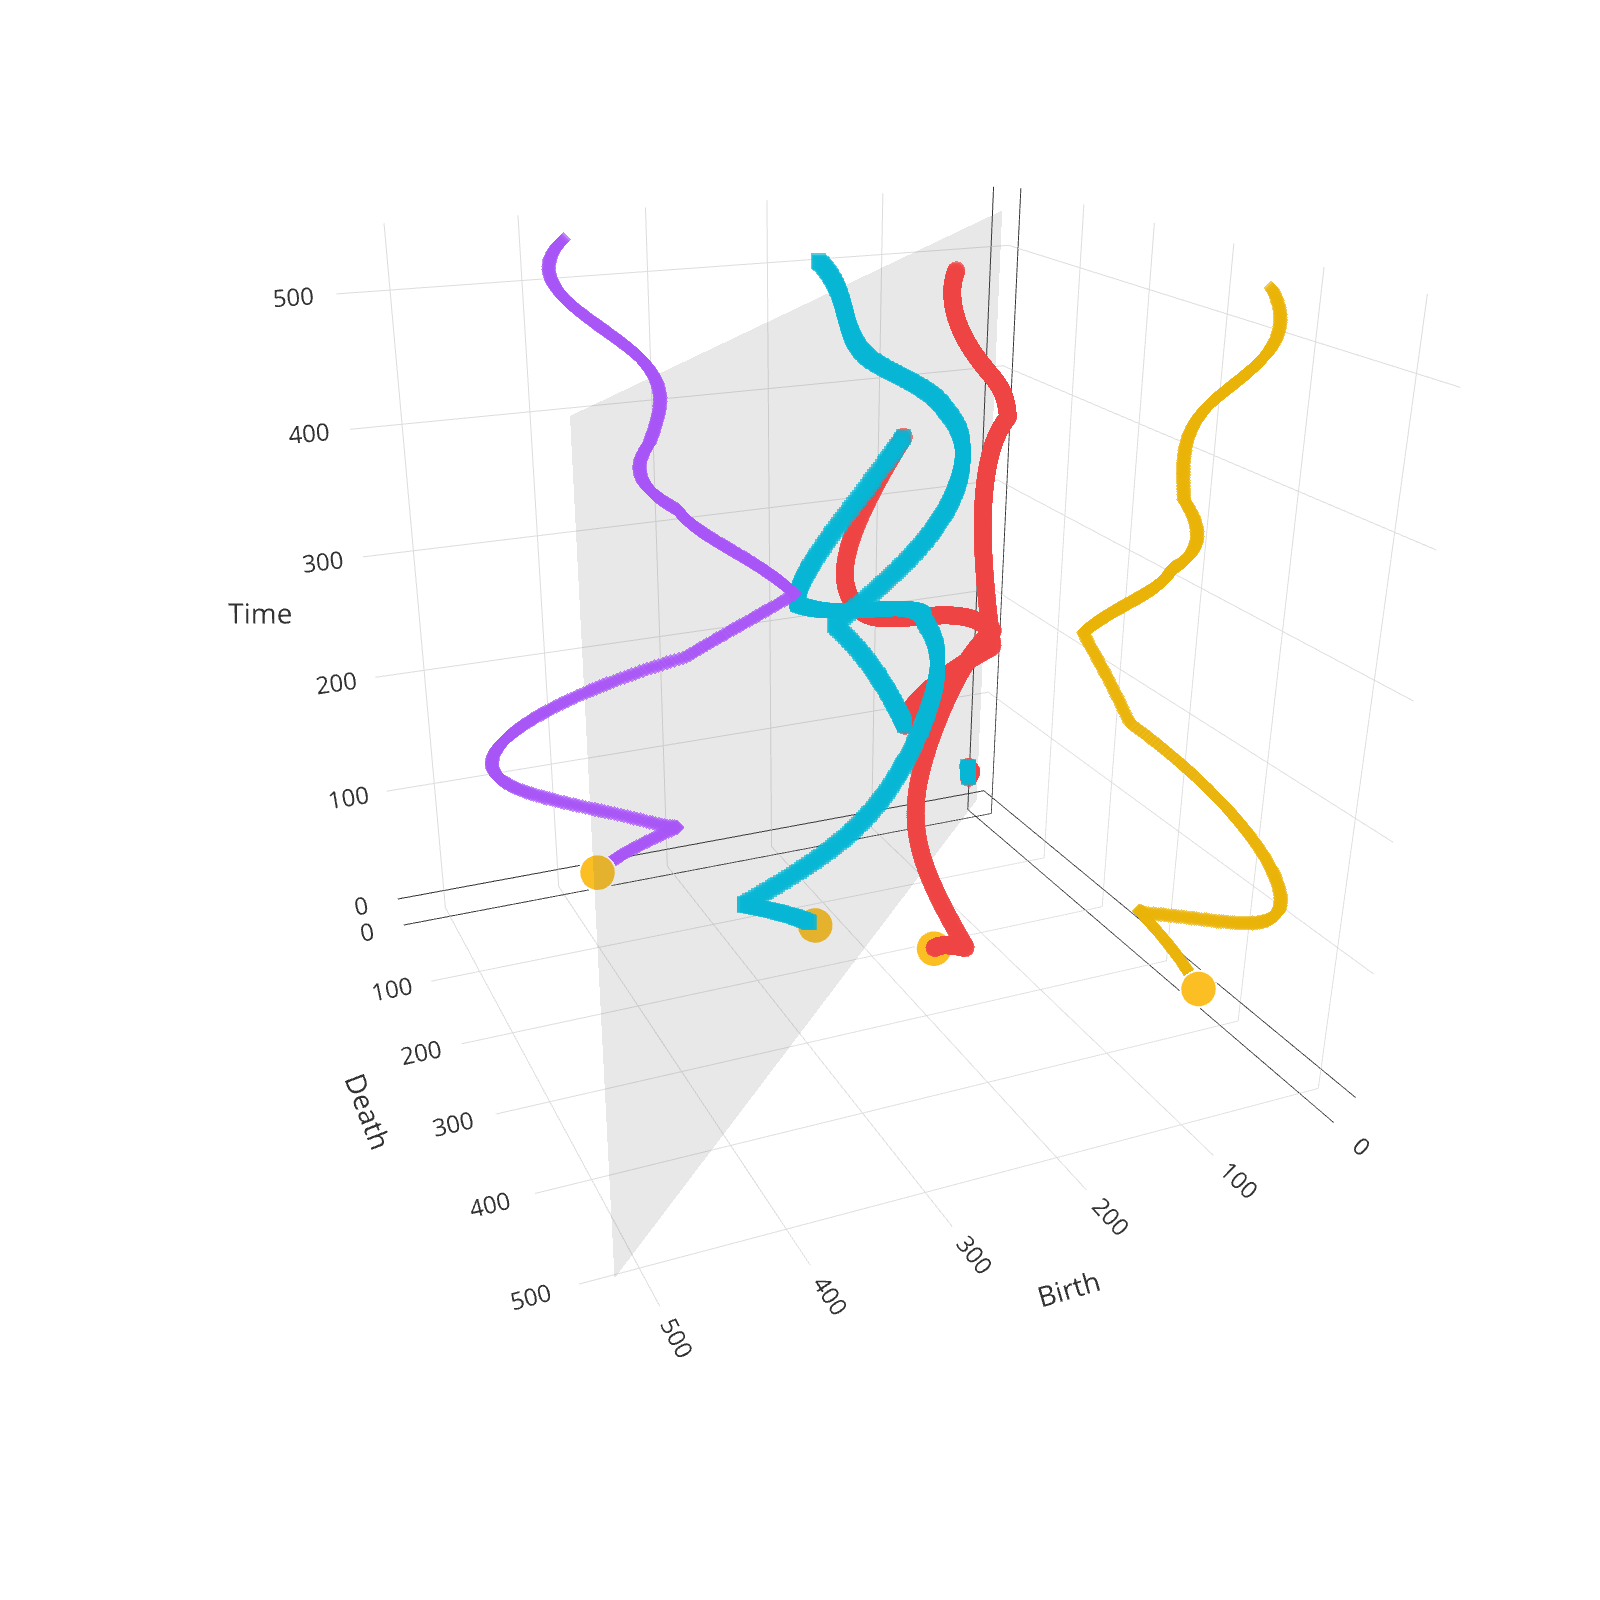
\includegraphics[width=\linewidth]{vin_spline.png}
            \end{figure}
        \end{column}
    \end{columns}
\end{frame}

%----------------------------------------------------------------------------------------

\section{Outlook}

\begin{frame}{Outlook and Future Work}
    \begin{itemize}
        \item Currently supports \textbf{2D only} --- future extensions to higher dimensions.
        \pause
        \item The tool provides geometric intuition for the theory developed in Chambers et al.\ [SODA 2026] on braiding and monodromy in vineyards.
        \pause
        \item We invite the community to \textbf{test the tool} and provide feedback!
    \end{itemize}

    \bigskip
    \centering
    \Large
    \url{https://www.rohitroy.me/symmetry-set-visualizer/bouquet2d.html}
\end{frame}

%----------------------------------------------------------------------------------------

\begin{frame}[plain]
	\begin{center}
		{\Huge Thank You!}

		\bigskip\bigskip

		{\LARGE Questions?}

        \bigskip

        \normalsize
        \url{https://www.rohitroy.me/symmetry-set-visualizer/bouquet2d.html}
	\end{center}
\end{frame}

%----------------------------------------------------------------------------------------

\end{document}
